%
%
% UCSD Doctoral Dissertation Template
% -----------------------------------
% https://github.com/ucsd-thesis/ucsd-thesis
%
%
% ----------------------------------------------------------------------
% WARNING:
%
%   This template has not endorced by OGS or any other official entity.
%   The official formatting guide can be obtained from OGS.
%   It can be found on the web here:
%   http://grad.ucsd.edu/_files/academic-affairs/Dissertations_Theses_Formatting_Manual.pdf
%
%   No guaranty is made that this LaTeX class conforms to the official UCSD guidelines.
%   Make sure that you check the final document against the Formatting Manual.
%
%   That being said, this class has been routinely used for successful
%   publication of doctoral theses.
%
%   The ucsd.cls class files are only valid for doctoral dissertations.
%
%
% ----------------------------------------------------------------------
% GETTING STARTED:
%
%   Lots of information can be found on the project wiki:
%   http://code.google.com/p/ucsd-thesis/wiki/GettingStarted
%
%
%   To make a pdf from this template use the command:
%     pdflatex template
%
%
%   To get started please read the comments in this template file
%   and make changes as appropriate.
%
%   If you successfully submit a thesis with this package please let us
%   know.
%
%
% ----------------------------------------------------------------------
% KNOWN ISSUES:
%
%   Currently only the 12pt size conforms to the UCSD requirements.
%   The 10pt and 11pt options make the footnote fonts too small.
%
%
% ----------------------------------------------------------------------
% HELP/CONTACT:
%
%   If you need help try the ucsd-thesis google group:
%   http://groups.google.com/group/ucsd-thesis
%
%
% ----------------------------------------------------------------------
% BUGS:
%
%   Please report all bugs at:
%   https://github.com/ucsd-thesis/ucsd-thesis/issues
%
%
% ----------------------------------------------------------------------
% More control of the formatting of your thesis can be achieved through
% modifications of the included LaTeX class files:
%
%   * ucsd.cls    -- Class file
%   * uct10.clo   -- Configuration files for font sizes 10pt, 11pt, 12pt
%     uct11.clo
%     uct12.clo
%
% ----------------------------------------------------------------------



% Setup the documentclass
% default options: 12pt, oneside, final
%
% fonts: 10pt, 11pt, 12pt -- are valid for UCSD dissertations.
% sides: oneside, twoside -- note that two-sided theses are not accepted
%                            by OGS.
% mode: draft, final      -- draft mode switches to single spacing,
%                            removes hyperlinks, and places a black box
%                            at every overfull hbox (check these before
%                            submission).
% chapterheads            -- Include this if you want your chapters to read:
%                              Chapter 1
%                              Title of Chapter
%
%                            instead of
%                              1 Title of Chapter
\documentclass[12pt,chapterheads]{ucsd}

% Include all packages you need here.
% Some standard options are suggested below.
%
% See the project wiki for information on how to use
% these packages. Other useful packages are also listed there.
%
%   http://code.google.com/p/ucsd-thesis/wiki/GettingStarted



%% AMS PACKAGES - Chances are you will want some or all
%    of these if writing a dissertation that includes equations.
%  \usepackage{amsmath, amscd, amssymb, amsthm}

%% GRAPHICX - This is the standard package for
%    including graphics for latex/pdflatex.
\usepackage{scrextend}
\usepackage{pslatex}
\usepackage{graphicx}
\usepackage{amsmath}
\usepackage{amsfonts}
\usepackage{float}
\usepackage{url}
\usepackage{makecell}
\usepackage{xcolor}

%% CAPTION
% This overrides some of the ugliness in ucsd.cls and
% allows the text to be double-spaced while letting figures,
% tables, and footnotes to be single-spaced--all OGS requirements.
% NOTE: Must appear after graphics and ams math
\makeatletter
\gdef\@ptsize{2}% 12pt documents
\let\@currsize\normalsize
\makeatother
\usepackage{setspace}
\doublespace
\usepackage[font=small, width=0.9\textwidth]{caption}

%% SUBFIG - Use this to place multiple images in a
%    single figure.  Subfig will handle placement and
%    proper captioning (e.g. Figure 1.2(a))
% \usepackage{subfig}

%% TIMES FONT - replacements for Computer Modern
%%   This package will replace the default font with a
%%   Times-Roman font with math support.
% \usepackage[T1]{fontenc}
% \usepackage{mathptmx}

%% INDEX
%   Uncomment the following two lines to create an index:
\usepackage{makeidx}
\makeindex
%   You will need to uncomment the \printindex line near the
%   bibliography to display the index.  Use the command
% \index{keyword}
%   within the text to create an entry in the index for keyword.
%   To compile a LaTeX document with an index the 'makeindex'
%   command will need to be run.  See the wiki for more details.

%% HYPERLINKS
%   To create a PDF with hyperlinks, you need to include the hyperref package.
%   THIS HAS TO BE THE LAST PACKAGE INCLUDED!
%   Note that the options plainpages=false and pdfpagelabels exist
%   to fix indexing associated with having both (ii) and (2) as pages.
%   Also, all links must be black according to OGS.
%   See: http://www.tex.ac.uk/cgi-bin/texfaq2html?label=hyperdupdest
%   Note: This may not work correctly with all DVI viewers (i.e. Yap breaks).
%   NOTE: hyperref will NOT work in draft mode, as noted above.

% \usepackage[colorlinks=true, pdfstartview=FitV,
%             linkcolor=black, citecolor=black,
%             urlcolor=black, plainpages=false,
%             pdfpagelabels]{hyperref}
% \hypersetup{ pdfauthor = {Your Name Here},
%              pdftitle = {The Title of The Dissertation},
%              pdfkeywords = {Keywords for Searching},
%              pdfcreator = {pdfLaTeX with hyperref package},
%              pdfproducer = {pdfLaTeX} }
% \urlstyle{same}
% \usepackage{bookmark}


%% CITATIONS
% Sets citation format
% and fixes up citations madness
\usepackage{microtype}  % avoids citations that hang into the margin


%% FOOTNOTE-MAGIC
% Enables footnotes in tables, re-referencing the same footnote multiple times.
\usepackage{footnote}
\makesavenoteenv{tabular}
\makesavenoteenv{table}


%% TABLE FORMATTING MADNESS
% Enable all sorts of fun table tricks
\usepackage{rotating}  % Enables the sideways environment (NCPW)
\usepackage{array}  % Enables "m" tabular environment http://ctan.org/pkg/array
\usepackage{booktabs}  % Enables \toprule  http://ctan.org/pkg/array

\usepackage{amsmath,amsfonts,amsthm,bm}
\usepackage{gensymb}



\usepackage{verbatim}

\usepackage[toc,nopostdot,style=alttree]{glossaries}
\glssetwidest{PERMANOVAX}% widest name
\makeglossaries
\newacronym{ad}{AD}{Atopic Dermatitis}
\newacronym{alr}{alr}{Additive Log-ratio}
\newacronym{ancom}{ANCOM}{Analysis of Composition of Microbiomes}
\newacronym{biom}{BIOM}{Biological Observation Matrix}
\newacronym{ca}{PCA}{Correspondence Analysis}
\newacronym{cf}{CF}{Cystic Fibrosis}
\newacronym{clr}{clr}{Center Log-ratio}
\newacronym{embad}{EMBAD}{Earth Mover Band Aware Distance)}
\newacronym{fp}{FP}{False Positive}
\newacronym{fn}{FN}{False Negative}
\newacronym{hgt}{HGT}{Horizontal Gene Transfer}
\newacronym{ilr}{ILR}{Isometric Log-ratio}
\newacronym{lse}{LSE}{Log sum exponential}
\newacronym{otu}{OTU}{Operational Taxonomic Unit}
\newacronym{pca}{PCA}{Principal Component Analysis}
\newacronym{pcoa}{PCoA}{Principal Coordinates Analysis}
\newacronym{pcm}{PCM}{Phylogenetic comparative methods}
\newacronym{pgls}{PGLS}{Phylogenetic Generalized Least Squares}
\newacronym{qiime}{QIIME}{Quantitative Insights into Microbial Ecology}
\newacronym{qpcr}{qPCR}{Quantitative Polymerase Chain Reaction}
\newacronym{permanova}{PERMANOVA}{Permutational Multivariate Analysis of Variance}
\newacronym{rrna}{rRNA}{Ribosomal RNA}
\newacronym{scorad}{SCORAD}{Scoring Atopic Dermatitis}
\newacronym{zig}{ZIG}{Zero Inflated Gaussian}



\begin{document}

%% FRONT MATTER
%
%  All of the front matter.
%  This includes the title, degree, dedication, vita, abstract, etc..
%  Modify the file template_frontmatter.tex to change these pages.

\title{Making sense of microbial populations from representative samples}

\author{James T. Morton}
\degreeyear{2018}

% Master's Degree theses will NOT be formatted properly with this file.
\degreetitle{Doctor of Philosophy}

\field{Computer Science}

\chair{Professor Rob Knight}
% Uncomment the next line iff you have a Co-Chair
% \cochair{Professor Cochair Semimaster}
%
% Or, uncomment the next line iff you have two equal Co-Chairs.
%\cochairs{Professor Chair Masterish}{Professor Chair Masterish}

%  The rest of the committee members  must be alphabetized by last name.
\othermembers{
Professor Pieter Dorrestein\\
Professor Rachel Dutton\\
Professor Yoav Freund\\
Professor Siavash Mirarab
}
\numberofmembers{5} % |chair| + |cochair| + |othermembers|


%% START THE FRONTMATTER
%
\begin{frontmatter}

%% TITLE PAGES
%
%  This command generates the title, copyright, and signature pages.
%
\makefrontmatter

%% DEDICATION
%
%  You have three choices here:
%    1. Use the ``dedication'' environment.
%       Put in the text you want, and everything will be formated for
%       you. You'll get a perfectly respectable dedication page.
%
%
%    2. Use the ``mydedication'' environment.  If you don't like the
%       formatting of option 1, use this environment and format things
%       however you wish.
%
%    3. If you don't want a dedication, it's not required.
%
%
\begin{dedication}
  To my friends and family who paved the road and lit the journey.
\end{dedication}


% \begin{mydedication} % You are responsible for formatting here.
%   \vspace{1in}
%   \begin{flushleft}
% 	To me.
%   \end{flushleft}
%
%   \vspace{2in}
%   \begin{center}
% 	And you.
%   \end{center}
%
%   \vspace{2in}
%   \begin{flushright}
% 	Which equals us.
%   \end{flushright}
% \end{mydedication}



%% EPIGRAPH
%
%  The same choices that applied to the dedication apply here.
%
\begin{epigraph} % The style file will position the text for you.
  \emph{The `paradox' is only a conflict between reality and your feeling of what reality `ought to be'}\\
  ---Richard Feynman
\end{epigraph}

% \begin{myepigraph} % You position the text yourself.
%   \vfil
%   \begin{center}
%     {\bf Think! It ain't illegal yet.}
%
% 	\emph{---George Clinton}
%   \end{center}
% \end{myepigraph}


%% SETUP THE TABLE OF CONTENTS
%
\tableofcontents

%%
%% This block was needed to re-format the title of the glossary to match the
%% headings of the list of figures and list of tables.
%%
%% start hack:
\renewcommand{\glossarysection}[2][]{
\newpage
\noindent
\centerline{LIST OF ABBREVIATIONS}
\addcontentsline{toc}{chapter}{List of Abbreviations}
}
%% end hack
\printglossary[title=List of Abbreviations,toctitle=List of Abbreviations,nonumberlist ]

\listoffigures  % Comment if you don't have any figures
\listoftables   % Comment if you don't have any tables


%% ACKNOWLEDGEMENTS
%
%  While technically optional, you probably have someone to thank.
%  Also, a paragraph acknowledging all coauthors and publishers (if
%  you have any) is required in the acknowledgements page and as the
%  last paragraph of text at the end of each respective chapter. See
%  the OGS Formatting Manual for more information.
%
\begin{acknowledgements}
  First, I would like to acknowledge Rob Knight, for his guidance that enabled me to
  grow as a person as well as a scientist.  This work was largely enabled by him and
  I am greatly thankful for his support.

  I would like to thank my committee members Pieter Dorrestein, Yoav Freund,
  Siavash Mirarab and Rachel Dutton not only for providing feedback for this
  thesis, but also for fostering years of collaborative science.

  This work couldn't have been done with out the strong support of the members of the
  Knight lab. Many thanks to the individuals responsible for the finances, logistics,
  and computational hardware maintainence that ultimately facilitated the sharing
  of ideas across public venues, namely Ulla Westerman, Jerry Kennedy, Gail Ackermann,
  Jeff DeReus, Michiko Souza, and Sarah Adams.  I would also like to acknowledge the
  multiple individuals that served as mentors, namely Jon Sanders, Daniel McDonald,
  Antonio Gonzalez, Yoshiki Vazquez-baeza, Zhenjiang Xu, Amnon Amir, Albert Barberán,
  Luke Thompson, Justine Debelius, Sejin Song, Jessica Metcalf, Greg Humphrey and Rob Quinn.
  My fellow peers brought the excitment into the lab, making my PhD experience
  thoroughly enjoyable, in particular Lisa Marotz, Qiyun Zhu, Stefan Janssen, Georg Loss,
  Anupriya Tripathi, Alison Vrbanac, Serene Lingjing Jiang, Antony Pearson,
  Peter Edge, Benjamin Pullman, Mingxun Wang, Richardo Silva, Alexander Aksenov,
  Louis-Felix Nothias-Scaglia and Brooke Anderson. Among the many collaborators,
  colleagues and mentors outside of UCSD responsible for contributing to
  this body of work, I would especially like to acknowledge Anna Edlund, Alex Washburne,
  Justin Silverman, John Karro, Iddo Friedberg, Manuel Lladser, Christopher Lowry,
  Noah Fierer, Benjamin Langmead, Jeff Leek and Susan Holmes for their
  thought-provoking insights.

  Finally, I would like to thank my friends and family for their love and support.
  In particular, my parents Jade and John Morton for their drive and care early
  on distilling my love in engineering, mathematics and science.  Rachael Morton
  for being a loveable sister and an angel on my shoulder.  And Juer
  Song, who is my pillar, my pillow and my greatest companion.

  Chapter 1, in full, is a reprint of the material as it appears in
  ``Methods for phylogenetic analysis of microbiome data''
  Alex D. Washburne, James T. Morton, Jon Sanders, Daniel McDonald,
  Qiyun Zhu, Angela M. Oliverio, Rob Knight  \emph{Nature Microbiology} 3, 2018. The dissertation author was the primary investigator and co-first author of this paper.

  Chapter 2, in full, is a reprint of the material as it appears in
  ``Uncovering the Horseshoe Effect in Microbial Analyses''
  James T. Morton, Liam Toran, Anna Edlund, Jessica L. Metcalf,
  Christian Lauber, Rob Knight \emph{mSystems}, 2, 2017.  The dissertation author was the primary investigator and first author of this paper.

  Chapter 3, in full, is a reprint of the material as it appears in
  ``Balance Trees Reveal Microbial Niche Differentiation''
  James T. Morton, Jon Sanders, Robert A. Quinn, Daniel McDonald, Antonio Gonzalez,
  Yoshiki Vázquez-Baeza, Jose A. Navas-Molina, Se Jin Song, Jessica L. Metcalf,
  Embriette R. Hyde, Manuel Lladser, Pieter C. Dorrestein, Rob Knight
  \emph{mSystems}, 2, 2017.  The dissertation author was the primary investigator and first author of this paper.

  Chapter 4 has been submitted for publication of the material as it may appear in
  Nature Biotechnology, 2019 ``Establishing microbial measurement standards with reference frames''
  James T. Morton,  Clarisse Marotz, Justin Silverman, Alex Washburne, Livia S. Zaramela,
  Anna Edlund, Karsten Zengler, Rob Knight. The dissertation author was the primary investigator and first author of this paper.


\end{acknowledgements}


%% VITA
%
%  A brief vita is required in a doctoral thesis. See the OGS
%  Formatting Manual for more information.
%
\begin{vitapage}
\begin{vita}

  \item[2014] B.~S. in Computer Science \emph{cum laude}, Miami University, OH
  \item[2014] B.~S. in Mathematics and Statistics \emph{cum laude}, Miami University, OH
  \item[2014] B.~S. in Electrical Engineering \emph{cum laude}, Miami University, OH
  \item[2014] B.~S. in Engineering Physics \emph{cum laude}, Miami University, OH
  \item[2018] Ph.~D. in Computer Science, University of California San Diego
\end{vita}
\begin{publications}
    \item \textsl{Author names marked with $\dagger$ indicate shared first co-authorship}.

    \item $\dagger$Alex D. Washburne, \textbf{$\dagger$James T. Morton}, Jon Sanders, Daniel McDonald, Qiyun Zhu, Angela M. Oliverio, Rob Knight  ``Methods for phylogenetic analysis of microbiome data'' \emph{Nature Microbiology} 3, 2018

    \item  \textbf{James T. Morton}, Liam Toran, Anna Edlund, Jessica L. Metcalf, Christian Lauber, Rob Knight ``Uncovering the Horseshoe Effect in Microbial Analyses'' \emph{mSystems}, 2, 2017

    \item \textbf{James T. Morton}, Jon Sanders, Robert A. Quinn, Daniel McDonald, Antonio Gonzalez, Yoshiki Vázquez-Baeza, Jose A. Navas-Molina, Se Jin Song, Jessica L. Metcalf, Embriette R. Hyde, Manuel Lladser, Pieter C. Dorrestein, Rob Knight ``Balance Trees Reveal Microbial Niche Differentiation'' \emph{mSystems}, 2, 2017

    \textsl{The following publications were not included as part of this dissertation, but were also significant byproducts of my doctoral training.}
\item  Stefan O Reber, Philip H  Siebler, Nina C  Donner, \textbf{James T Morton}, David G  Smith, Jared M  Kopelman, Kenneth R  Lowe, Kristen J  Wheeler, James H  Fox, James E  Hassell,  ``Immunization with a heat-killed preparation of the environmental bacterium Mycobacterium vaccae promotes stress resilience in mice'' \emph{Proceedings of the National Academy of Sciences}, 113, 2016

    \item  Jack A Gilbert, Robert A  Quinn, Justine  Debelius, Zhenjiang Z  Xu, James  Morton, Neha  Garg, Janet K  Jansson, Pieter C  Dorrestein, Rob  Knight,  ``Microbiome-wide association studies link dynamic microbial consortia to disease'' \emph{Nature}, 535, 2016

    \item  Yoshiki Vázquez-Baeza, Antonio  Gonzalez, Larry  Smarr, Daniel  McDonald, \textbf{James T Morton}, Jose A  Navas-Molina, Rob  Knight,  ``Bringing the dynamic microbiome to life with animations'' \emph{Cell host \& microbe}, 21, 2017


    \item  Albert Barberán, Robert R  Dunn, Brian J  Reich, Krishna  Pacifici, Eric B  Laber, Holly L  Menninger, \textbf{James T Morton}, Jessica B  Henley, Jonathan W  Leff, Shelly L  Miller,  ``The ecology of microscopic life in household dust'' \emph{Proc. R. Soc. B}, 282, 2015

    \item  Erin M Hill‐Burns, Justine W  Debelius, \textbf{James T Morton}, William T  Wissemann, Matthew R  Lewis, Zachary D  Wallen, Shyamal D  Peddada, Stewart A  Factor, Eric  Molho, Cyrus P  Zabetian,  ``Parkinson's disease and Parkinson's disease medications have distinct signatures of the gut microbiome'' \emph{Movement disorders}, 32, 2017


    \item  Amnon Amir, Daniel  McDonald, Jose A  Navas-Molina, Justine  Debelius, \textbf{James T Morton}, Embriette  Hyde, Adam  Robbins-Pianka, Rob  Knight,  ``Correcting for microbial blooms in fecal samples during room-temperature shipping'' \emph{MSystems}, 2, 2017

    \item  Amnon Amir, Daniel  McDonald, Jose A  Navas-Molina, Evguenia  Kopylova, \textbf{James T Morton}, Zhenjiang Zech  Xu, Eric P  Kightley, Luke R  Thompson, Embriette R  Hyde, Antonio  Gonzalez,  ``Deblur rapidly resolves single-nucleotide community sequence patterns'' \emph{MSystems}, 2, 2017

    \item  Alison Vrbanac, Justine W  Debelius, Lingjing  Jiang, \textbf{James T Morton}, Pieter  Dorrestein, Rob  Knight,  ``An Elegan (t) Screen for Drug-Microbe Interactions'' \emph{Cell host \& microbe}, 21, 2017

    \item  Sian MJ Hemmings, Stefanie  Malan-Müller, Leigh L  van den Heuvel, Brittany A  Demmitt, Maggie A  Stanislawski, David G  Smith, Adam D  Bohr, Christopher E  Stamper, Embriette R  Hyde, \textbf{James T Morton},  ``The microbiome in posttraumatic stress disorder and trauma-exposed controls: an exploratory study'' \emph{Psychosomatic medicine}, 79, 2017

    \item  Laura-Isobel McCall, \textbf{James T Morton}, Jean A  Bernatchez, Jair Lage  de Siqueira-Neto, Rob  Knight, Pieter C  Dorrestein, James H  McKerrow,  ``Mass spectrometry-based chemical cartography of a cardiac parasitic infection'' \emph{Analytical chemistry}, 89, 2017

    \item  Yoshiki Vázquez-Baeza, Chris  Callewaert, Justine  Debelius, Embriette  Hyde, Clarisse  Marotz, \textbf{James T Morton}, Austin  Swafford, Alison  Vrbanac, Pieter C  Dorrestein, Rob  Knight,  ``Impacts of the human gut microbiome on therapeutics'' \emph{Annual review of pharmacology and toxicology}, 58, 2018

    \item  Jessica L Metcalf, Se Jin  Song, \textbf{James T Morton}, Sophie  Weiss, Andaine  Seguin-Orlando, Frédéric  Joly, Claudia  Feh, Pierre  Taberlet, Eric  Coissac, Amnon  Amir,  ``Evaluating the impact of domestication and captivity on the horse gut microbiome'' \emph{Scientific reports}, 7, 2017

    \item  Lingjing Jiang, Amnon  Amir, \textbf{James T Morton}, Ruth  Heller, Ery  Arias-Castro, Rob  Knight,  ``Discrete false-discovery rate improves identification of differentially abundant microbes'' \emph{MSystems}, 2, 2017

    \item  Clifford A Kapono, \textbf{James T Morton}, Amina  Bouslimani, Alexey V  Melnik, Kayla  Orlinsky, Tal Luzzatto  Knaan, Neha  Garg, Yoshiki  Vázquez-Baeza, Ivan  Protsyuk, Stefan  Janssen,  ``Creating a 3D microbial and chemical snapshot of a human habitat'' \emph{Scientific reports}, 8, 2018

    \item  Daniel McDonald, Embriette  Hyde, Justine W  Debelius, \textbf{James T Morton}, Antonio  Gonzalez, Gail  Ackermann, Alexander A  Aksenov, Bahar  Behsaz, Caitriona  Brennan, Yingfeng  Chen,  ``American Gut: an Open Platform for Citizen Science Microbiome Research'' \emph{mSystems}, 3, 2018


    \item  Robert A Quinn, William  Comstock, Tianyu  Zhang, \textbf{James T Morton}, Ricardo  da Silva, Alda  Tran, Alexander  Aksenov, Louis-Felix  Nothias, Daniel  Wangpraseurt, Alexey V  Melnik,  ``Niche partitioning of a pathogenic microbiome driven by chemical gradients'' \emph{Science advances}, 4, 2018
\end{publications}
\end{vitapage}


%% ABSTRACT
%
%  Doctoral dissertation abstracts should not exceed 350 words.
%   The abstract may continue to a second page if necessary.
%
\begin{abstract}
Microbiomes make up the vast majority of life on Earth, and we are just beginning to understand how to
study them using high-throughput omics.  However, analysis of microbial populations is complicated by
numerous statistical challenges.  We first outline these challenges in the context of phylogenetically
aware methods, then focus on two concepts: the horseshoe effect and compositionality.

The horseshoe effect is a phenomenon that can lead to horseshoe patterns appearing in low dimensional
representations of high dimensional data.  For multiple decades, this pattern confounded ecologists
when studying populations across multiple environmental conditions.  Here, we show that the
horseshoe effect arises from distance saturation, and can indicative of microbial population
displacement. This phenomenon is illustrated across a soil study and a
decomposition study.

In the second part of the thesis, we will discuss identifiability due to representative sampling,
also known as compositionality. Statistical laws have shown that it's possible to obtain
unbiased estimators for population proportions from representative samples.
However, based on representative samples alone, it is not possible to determine which species abundances
have grown or declined, since there is an infinite number of outcomes that can explain
the same change in proportions. In the biological sciences, this problem is also known as the
differential abundance problem, which is critical for determining which microbes have been altered across
experimental outcomes. Here, we show that in order to estimate which species have been altered,
the total population size needs to be estimated.

We present two workarounds to this problem that ultimately negating the need to estimate total
population size. The first solution is using ratios, analogous to concentrations in chemistry.
We will showcase the usefulness of this technique on a soils study and a cystic fibrosis study.
The second solution is using ranks as a proxy to feature importances. Rather than attempting to
compute absolute change, we can compute relative change, ultimately ranking which microbes have
increased or decreased the most across different experimental conditions.
We show how these ranks can be computed using multinomial regression and can
facilitate reproducible findings in the context of oral microbial communities and atopic dermatitis.
\end{abstract}


\end{frontmatter}



%% DISSERTATION

% A common strategy here is to include files for each of the chapters. I.e.,
% Place the chapters is separate files:
%   chapter1.tex, chapter2.tex
% Then use the commands:
%   \include{chapter1}
%   \include{chapter2}
%
% Of course, if you prefer, you can just start with
%   \chapter{My First Chapter Name}
% and start typing away.

\chapter{Methods for phylogenetic analysis of microbiome data}
\glsresetall
How does knowing the evolutionary history of microbes affect our analysis of microbiological datasets? Depending on the research question, the common ancestry of microbes can be a source of confounding variation or can be a scaffolding used for inference. For example, when performing regression on traits the common ancestry is a source of dependence among observations, whereas when searching for clades with correlated abundances the common ancestry is the scaffolding for inference. The common ancestry of microbes and their genes is organized in trees – phylogenies – which can and should be incorporated into the analysis of microbial datasets.\par
While there has been a recent expansion of phylogenetically informed analytical tools, little guidance exists for which method best answers which biological questions. Here, we review methods for phylogeny-aware analyses of microbiome datasets, considerations for choosing the appropriate method, and challenges inherent in these methods.  We introduce a conceptual organization of these tools, breaking them down into phylogenetic comparative methods, ancestral state reconstruction, analysis of phylogenetic variables, and analysis of phylogenetic distances. Careful consideration of the research question and ecological and evolutionary assumptions will help researchers choose a phylogeny and appropriate methods to produce novel, accurate, and biologically informative insights.
\section{Introduction}
High-throughput sequencing yields information about microbial communities in quantities that outstrip our ability to make sense of it. Most microbial taxa have never been cultivated or experimentally characterized. For many, we have only sequence fragments, whole genome sequence data for a few distant relatives, and a tree capturing the microbes' evolutionary histories. How can we organize and analyze the deluge of information about uncharacterized microbes and their sequence fragments?\par
Two main tools for organizing the diversity of life are the taxonomy and the phylogeny. The taxonomy classifies a microbe based on a hierarchy of taxonomic names ranging from one of three domains (Bacteria, Archaea and Eukarya) to one of several million species. The phylogeny is an estimation of the microbes' evolutionary history which classifies every organism by a series of splits corresponding to estimated events in which a most recent common ancestor speciated to form two daughter species.\par
Microbial taxonomy and phylogeny may eventually be equivalent, with every clade in the phylogeny having a taxonomic name. However, contemporary taxonomic classification is coarse relative to the phylogeny; modern taxonomic labels categorize a small fraction of the branches in the phylogeny. For the time being, the phylogeny is a more detailed source of knowledge about the common ancestry of microbes.\par

Phylogenies are a tool to organize and understand the microbial world\cite{martiny_phylogenetic_microbiome} \cite{hug_tree_of_life}. Because related organisms tend to have similar characteristics, phylogenies can incorporate those characteristics into our analyses even if we can't measure them directly. Phylogenies are a scaffold to classify lineages and infer functional ecological traits, even for lineages that have not been classified taxonomically or physiologically. Microbial ecology can be accelerated by high-throughput classification and inferences made possible with phylogenies. Resource consumption \cite{tilman_resouce_competition}, habitat associations\cite{macarthur_bird_diversity} and species interactions\cite{may_ecosystem_stability}\cite{arditi_species_interact} are causes and consequences of traits, and using phylogenies to infer or implicitly work with traits may enhance our ability to manipulate microbial communities to impact human health \cite{hmp_structure}, biogeochemistry \cite{falkowski_microbial_chemistry}, and climate change \cite{bardgett_microbial_climate}.\par
How can a phylogeny assist analyses of microbiome data? Different research questions require different considerations about how to amend statistical analyses when considering a phylogeny. For example, studies testing associations between traits should consider the phylogeny as a source of dependence among observations, whereas studies looking for simpler ways of binning species should consider the phylogeny as a scaffolding for possible bins. There is a vast and growing literature on methods for analyzing phylogenetically-structured data, methods with subtle yet consequential differences in the questions they seek to answer. There is a need to simplify the diverse field into a set of conceptually distinct classes of methods and thereby provide a framework for instruction, comparison, and development of methods for analyzing phylogenetically-structured data.\par
In this review, we organize the field of phylogenetically-structured data analysis by discussing the major classes of methods. We first emphasize a fundamental issue in the field: the imperfection of estimated phylogenies. We then define four categories: (1) comparative methods, (2) ancestral state reconstruction and descendant trait imputation (3) variable analysis, and (4) phylogeny-aware distances (Table 1). Most statistical tools can be revisited for phylogeny-aware analyses, but the categories we cover capture the most commonly used and actively developed classes of methods. We discuss challenges of phylogenetically-aware analysis of microbiome data, including horizontal gene transfer (\gls{hgt}) and the choice of which genes to use when building phylogenies. By partitioning the literature into distinct conceptual classes of methods, we provide a common framework for the development and implementation of these important methods in microbiome data analysis.

\begin{table}[!ht]
        \caption[Comparison of different phylogentically aware methods.]{Comparison of different phylogentically aware methods. Different classes of methods for using the phylogeny in data analysis address different classes of questions. These methods can be summarized based on their use of given a dataset of abundance vectors, x, observed or imputed trait values, y, and the phylogeny, P. }

        \vspace{-0.25in}
        \begin{center}
                \begin{tabular}{|p{0.7in}|p{1.3in}|p{1.1in}|p{1.1in}|p{1.1in}|}
                        \hline
                        Class of Methods & Brief Description & Specific Example & General Formula & Highlighted Method \\
                        \hline
                        Comparative Methods &Find associations between traits, controlling for evolution on phylogeny & Is 16S \gls{rrna} gene copy number associated with growth rates in	vivo?& $y_{i}-g(Y)+\epsilon $
                        where

                        Conv $\left [ \epsilon  \right ]=f(P)$ & \gls{pgls}\cite{pgls}
                        Paired    \hspace{2cm}t-test\cite{martins_pcm} \\
                        \hline
                        Ancestral State Reconstruction & Impute trait values for historical
                        lineages in the phylogeny and use ancestral traits to impute trait
                        values for contemporary species & What is the best estimate of 16S \gls{rrna} gene copy number of
                        an \gls{otu} based on the 16S \gls{rrna} copy numbers of its relatives? & Infer features of $P|y $
                        Impute $y_{i,j}|y_{j}$ & PICRUSt\cite{picrust}  \\
                        \hline
                        Phylogenetic Variables & Use the phylogeny to construct	variables that are biologically
                        interpretable (for example, a clade's abundance) and simplify/summarize features in the
                        community & Which interior edges in P
                        separate taxa with different habitat associations? How does
                        Faith's phylogenetic diversity change with pH? &
                        Define variables:
                        $v_{i}= f_{i}(x,P)$  Analyse, interpret and combine $v_{i}$ & Diversity analyses
                        Taxonomic analyses Phylofactorization \cite{Washburne2017-up}
                        EdgePCA\cite{edgepca} Ph\gls{ilr}\cite{Silverman2016-he} \\
                        \hline
                        Phylogeny-Aware Distances & Use the phylogeny to construct distances between samples,
                        which can then be used to modify statistical tools for classification, regularized regression
                        and more & How different are two microbial communities? & Define distance
                        $d[x_{i},x_{j}]=K(x_{i},x_{j},P)$
                        Analyse and use to modify
                        various statistical methods & UniFrac\cite{unifrac, socolar_prey,
                          mccann_diversity, socolar_beta_diversity}\;
                        Inner product methods\cite{aitchison_statistics}, \cite{gloor_compositional_analysis}\\
                        \hline
                \end{tabular}
        \end{center}
        \label{tab:analysis3}
\end{table}

\section{Phylogenetic Inference}
The tree of life is not known; it is estimated, and accurate phylogenies improve accuracy of phylogenetically-structured data analysis. Microbial phylogenies are commonly estimated by collecting gene sequences, aligning sequences based on homologies, and using models of mutation to infer most-likely evolutionary histories. The estimated phylogeny can vary depending on which genes are sequenced, how sequence positions are aligned, which model of evolution is used, and the method for inferring histories. Errors in phylogenetic inference can propagate to errors in phylogenetically-structured data analysis. Here, we discuss the interplay between phylogenetic inference and phylogenetically-aware analyses; for a review of methods for phylogenetic inference, readers can consult focused reviews of that topic \cite{molecular_evolution, molecular_phylogenetics}.\par
One can construct a phylogeny for any gene, and different genes will vary in the number of species containing the gene, the accuracy of the phylogeny, and phylogenetic signal of a set of traits. The 16S \gls{rrna} gene is commonly used for phylogenetic inference in Bacteria and Archaea, but one could also construct a phylogeny for other genes such as beta lactamases and their relatives, yielding a phylogeny with edges along which antibiotic resistance traits arose \cite{molecular_evolution}. Microbial Eukaryotes likewise have many genes which can be used for phylogenetic inference, the 18S \gls{rrna} gene being most commonly used\cite{hillis_ribosome}. \par
The genes chosen for phylogenetic inference ultimately determine the set of traits correlated with the phylogeny. Bacterial genome trees generally correlate with the 16S \gls{rrna} gene (16S)-derived phylogenies\cite{snel_genome_phylogeny}, but the correlation between a 16S tree and gene content varies over lineages and phylogenetic depths\cite{zaneveld_ribosome}. \gls{hgt} disrupts the correlation between 16S trees and gene content by allowing bacteria with distant 16S genes to share common and consequential traits, such as pathogenicity islands and antibiotic resistance genes\cite{hall_lactamase,prokaryotic_evolution}. Moreover, the 16S sequence has multiple variable regions, and can vary among multiple copies within the same genome, complicating phylogenetic inference\cite{variability_16s}. More complicated scenarios, such as when epistasis underlies a functional ecological trait and one of the epistatic genes can be horizontally transmitted, prohibit a clear prescription for which gene's tree should be used for phylogenetic inference.\par
Different methods for analyzing phylogenetically-structured data use different features of the phylogeny. Distances and phylogenetic comparative methods which aggregate information over many branches in the phylogeny are more robust to errors in phylogenetic inference\cite{weighted_unifrac,robust_phylogenetic_regression} . Methods which rely on a few branches are more sensitive to errors in phylogenetic inference \cite{riesenfel_phylogeny}. For methods relying on a few internal nodes or branches, the uncertainty in phylogenetic inference – particularly the bootstrap support for the monophyly of critical branches\cite{felsenstein_confidence} – may be an important measure of uncertainty to incorporate into downstream data analysis. Where monophyly is crucial, researchers can collapse resolved nodes into polytomies to improve the bootstrap support across the whole tree. A more certain yet coarse-grained phylogeny may be preferable to a less certain yet fully resolved phylogeny.  Incorporating phylogenetic information has the capacity of drawing hypotheses on organisms never observed before.  While the vast majority of microbial life on the planet is not cultureable,phylogenetic analyses allow us to extrapolate and infer characteristics about unknown organisms based on closely related, cultureable organisms.
\section{Phylogenetic Comparative Methods}
Phylogenetic comparative methods (\gls{pcm}s) are used when comparing multiple traits across organisms. Closely related organisms often have similar traits due to inheritance from a common ancestor; such dependence of traits across organisms can affect tests of trait:trait and trait:habitat associations. \par
For example, we may find an association between 16S copy number (trait) and pH preference (habitat) through a correlation between 16S copy number and a measure of pH preference across 1,000 species of microbes (figure \ref{fig1a}a). Such an association could yield a false positive result if the taxa consist of a set of closely related of Acidobacteria with low 16S copy number and low pH preference, and a set of closely related Fusobacteria with high 16S copy number and a high pH preference\cite{variability_16s}. Intuitively, the phylogenetic signal of these traits reduces our sample size because the observed traits represent samples from two lineages, not 1,000 independent species. More rigorously, the phylogeny affects the covariance structure of residuals under null models of trait evolution. Robust tests of trait-associations are done using \gls{pcm}s\cite{grafen_regression} \cite{martins_pcm} (figure \ref{fig1a}b). \par
How does one account for dependence among trait observations? Generalized least squares can control for dependence among observations when performing regression. In generalized least squares, the residuals have an expected covariance under a null model and the covariance matrix is incorporated into least-squares calculations. For regression analyses, such as looking for associations between 16S copy number and habitat preference, phylogenetic generalized least squares\cite{blomberg_pgls} (\gls{pgls}; figure \ref{fig1a}) is a popular method using generalized least squares to correct for the expected covariance of residuals under null models of trait evolution along the branches of the phylogeny \cite{pagel_evolution}. \par
To implement \gls{pgls}, one first estimates the nature and magnitude of phylogenetic signal in the response variable. Pagel's $\lambda$ \cite{pagel_evolution} or Blomberg et al.'s $\kappa$ \cite{blomberg_test} are commonly used test statistics for phylogenetic signal. The phylogenetic signals from Pagel's $\lambda$, Blomberg's $\kappa$, or other metrics define covariance matrices of the residuals which can be used in generalized least squares (figure \ref{fig1a}b). For more complicated models of evolution, one can jointly estimate the parameters for the evolutionary model and the regression coefficients \cite{lavin_morphometrics}.\par
\gls{pcm}s extend to many statistical tests. Testing whether the volume of bacterial spores is smaller than the volume of daughter cells would involve a paired t-test, absent phylogenetic signal. A phylogenetic paired t-test\cite{lindenfors_test} was developed to account for phylogenetic signal in such tests. There are many models of trait evolution, metrics of phylogenetic signal, and methods to control for phylogenetic signal when comparing traits. A recent scholarly edition of modern \gls{pcm}s provides a review of the field and directions of current research\cite{pgls}.\par
\begin{figure}[H]
        \centering
        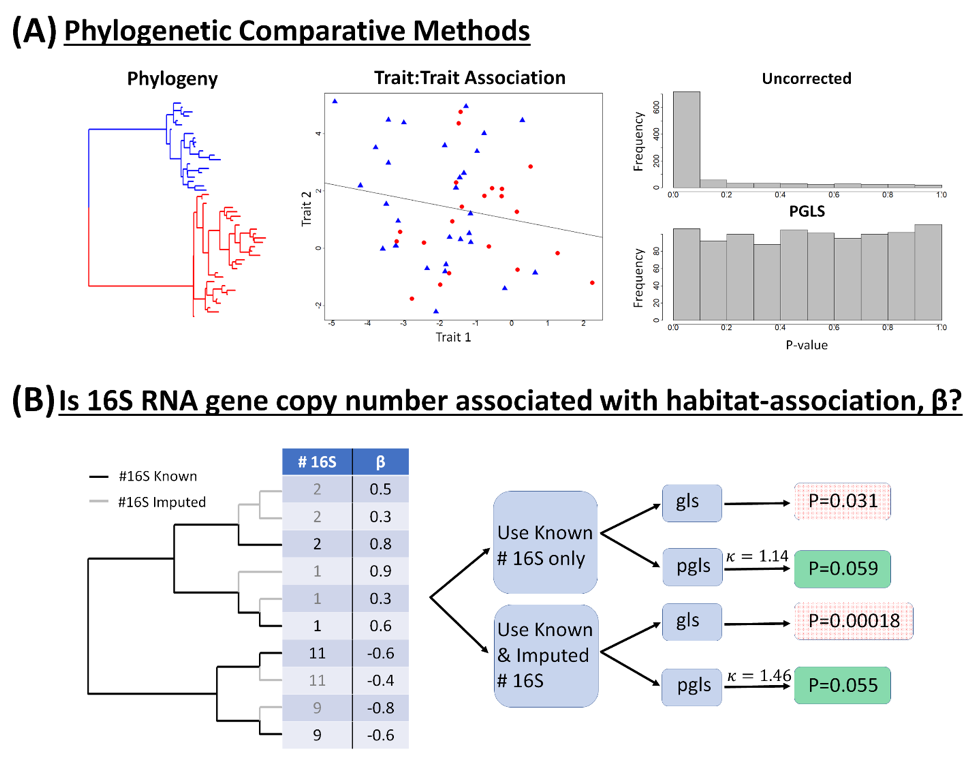
\includegraphics[width=1\textwidth]{ch1/figure1.png}
        \caption[Advantages of using phylogenetic comparative methods.]
        {Advantages of using phylogenetic comparative methods. Phylogenetic comparative methods control for the statistical dependence among traits resulting from evolution of traits along the phylogenetic tree. (A) An exaggerated phylogeny with two distantly related clades. If trait evolution is simulated as a random walk on the phylogeny, the two distantly related clades will drive covariances between traits. Failing to correct for the effects of random trait evolution can lead to a high false-positive rate. Methods such as phylogenetic generalized least squares (\gls{pgls}) correct for the residual covariance expected under random trait evolution and produce more accurate statistical tests of association. (B) \gls{pgls} should be used when testing associations between traits, even trait quantities such as regression coefficients from abundance~meta-data associations. To implement \gls{pgls}, a model of trait evolution needs to be assumed or estimated. Here, we estimate Blomberg's $\kappa$. \gls{pgls} should be used regardless whether the traits used are known or imputed through ancestral state reconstruction.\index{SanDiego}}
        \label{fig1a}
\end{figure}
\gls{pcm}s are not commonly used in microbiome studies, although a recent study\cite{bradley_phylogeny_correction} has employed \gls{pcm}s to identify genes associated with colonization of the human gut (trait:habitat). Failure to correct for phylogenetic dependence in tests of trait:trait and trait:habitat association can yield a high false-positive rate (figure \ref{fig1a}). To amend this, we recommend researchers familiarize themselves with and utilize \gls{pcm}s. Many methods can be implemented through the R packages \cite{ape} , phangorn \cite{phangorn}, phytools\cite{phytools}, picante\cite{picante}, caper \cite{caper}, Geiger \cite{geiger}, and phylglm\cite{phylglm}. In the supplemental online tutorial (https://knightlab-analyses.github.io/phylogenetic-tutorials/), we illustrate how these packages can be used to simulate trait evolution and test associations between traits. We also illustrate the sensitivity of these methods to \gls{hgt}.
\section{Ancestral State Reconstruction}
Estimating, or reconstructing, ancestral trait values assists imputation of traits in uncharacterized species and identification of historical lineages along which major trait differences arose. In studies of microorganisms, ancestral state reconstruction is commonly used to estimate genetic and metabolic profiles of extant communities using a set of reference genomes. In microbiome studies, this is commonly performed using PICRUSt\cite{picrust}, which uses pre-calculated ancestral state reconstructions to impute trait values, such as genes encoding glycoside hydrolase activity, for taxa whose traits are unknown.\par
PICRUSt operates on a phylogenetic tree, constructed from 16S sequences, connecting various sequenced genomes and environmental sequences. First, trait information observed in the sequenced genomes is used to infer ancestral trait profiles. Ancestral profiles are then used to predict the profiles of each organism in an environmental sample. An input sample's predicted metagenomic profile is then estimated by adding the product of \gls{otu} abundances in the sample and their corresponding profiles. Because this method relies strongly on the reference database, and the available sequenced genomes, it underperforms in environments where few or no genomes are known. Conversely, PICRUSt was able to predict the profiles of whole genome shotgun human fecal samples with a Spearman $R^2$ of $>$ 0.9 \cite{picrust}, suggesting that the microbial phylogeny is high predictive of microbial genome content.\par
The methodology underlying ancestral state reconstruction are very similar to phylogenetic comparative methods, as both require considering models of evolution \cite{ancestral_character_states}. Three main types of algorithms are used to connect the tree, traits, a model of evolution, and estimates of ancestral states given the model of evolution: maximum parsimony, maximum likelihood and Bayesian inference\cite{ancestral_character_states}. Maximum parsimony reconstructs ancestral states by minimizing the number of trait changes between the ancestor and the present descendants. This approach assumes that trait changes are slow, and does not account for scenarios involving rapid evolution. In addition, maximum parsimony treats all branches the same and minimizes the number of changes on each branch; this can be problematic, particularly if not all of the species have been observed \cite{ancestral_reconstruction}. Maximum likelihood and Bayesian inference improve on maximum parsimony by incorporating explicit models of evolution – such as a Brownian motion model of trait evolution along the tree - into the estimation of ancestral states. Rather than simply assuming that changes are rare, these methods can account for some changes occurring more frequently than others—for example, assuming synonymous substitutions are more frequent than non-synonymous substitutions—and fit parameters to these models given an estimated phylogeny.  However, maximum likelihood will often underestimate the number of changes within a single branch and can generate suboptimal results, particularly if the rate of evolution changes across the phylogeny \cite{simulation_comparison}. Bayesian approaches can compute evolutionary parameters across a deep sampling of possible evolutionary trees and evaluate more complex models of evolution that account for non-uniform rates of evolution. While Bayesian methods can generate more accurate results than maximum parsimony or maximum likelihood, they can be computationally expensive with large numbers of species.  Consequently, PICRUSt estimates microbial ancestral states using maximum parsimony or maximum likelihood. \par
As for phylogenetic comparative methods, estimates of ancestral states can be quickly confounded by \gls{hgt} (see supplemental online tutorial), and thus applications of these methods to microbial datasets should be performed with consideration of the observed rates of transfer for the gene families of interest.
\section{Analysis of phylogenetic variables}
While points on the Earth's surface can be located with three Cartesian (xyz) coordinates, we naturally describe locations using two spherical coordinates (latitude and longitude). A phylogeny, like a sphere, defines the map of biological data and suggests natural coordinates. Phylogenetic variables are used to reduce the dimension of community ecological data, simplify calculations of distances, and describe meaningful features and directions of change in communities (figure \ref{figa2}).
We coin the term “phylogenetic variables” to describe variables constructed using features in the phylogeny to aggregate, contrast, and summarize data of species in the phylogenetic tree (figure \ref{figa2}). Variables and distances are related, but contain distinct information: saying the city is east doesn't indicate how far it is, and saying a city is 80 kilometers away doesn't indicate which direction it is. Directions are described through phylogenetic variables (figure \ref{figa2}A), and the magnitude of changes is measured through distances (figure \ref{figa2}B). Phylogenetic variables include diversity metrics, taxonomic abundances, differences of abundance along all edges \cite{picante}, differences of abundances between clades (figures \ref{figa2}A, \ref{figa2}C, \ref{figa2}D) \cite{Washburne2017-up} \cite{Silverman2016-he}, and more. \par
\begin{figure}[H]
        \centering
        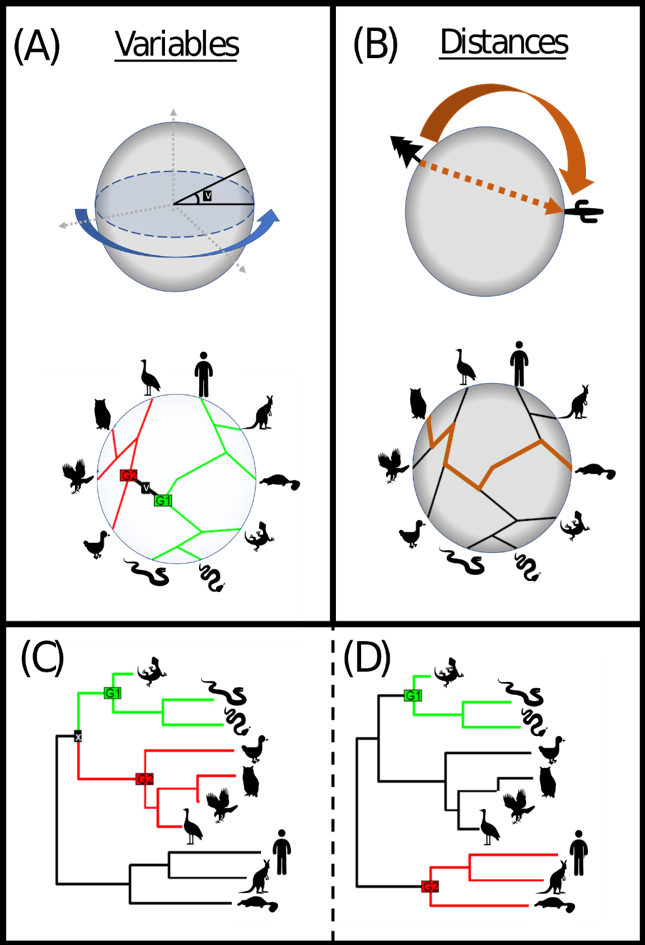
\includegraphics[width=0.7\textwidth]{ch1/figure2.png}
        \caption[A comparison between phylogenetic variable analysis and phylogenetic distances.]
        {A comparison between phylogenetic variable analysis and phylogenetic distances. Phylogenies define the geometry of community ecological data, much like a sphere defines the geometry of GPS data. (A) Changing variables can allow more natural descriptions of complex topologies. A spherical Earth motivates spherical coordinates. Phylogenetic variables use the tree as a scaffolding for constructing coordinates corresponding to phylogenetic features. Phylofactorization constructs coordinates contrasting groups, G1 and G2, separated by edges where traits such as flight arose. (B) A default path between two points is a straight line, but a more meaningful path on a sphere is “as the crow flies”. Likewise, phylogeny-aware distances such as UniFrac define evolutionary paths and their distances between one community to another. (C) Ph\gls{ilr} constructs coordinates contrasting sister clades. (D) The space of possible phylogenetic variables and distances is infinitely large. Researchers should consider the biological interpretability of novel variables and distances, and their ability to inform future studies.\index{SanDiego1}}
        \label{figa2}
\end{figure}
Phylogenetic variables simplify microbiome datasets by reducing the dimension of the data to a few variables carrying biological information. If a few monophyletic clades explain the majority of a microbiome dataset's variance along an environmental gradient, then there may be traits, shared among members of each clade, which are important determinants of abundance along the environmental gradient and underlie the observed community compositional changes.
The set of possible phylogenetic variables is infinitely large. Consequently, researchers must be deliberate in their choice of novel phylogenetic variables – what are important directions of change that carry implications for further research? Community changes along the direction of a phylogenetic variable, such as alpha diversity, does not necessarily convey useful biological information or immediate implications for future study design. Two common challenges in the analysis of phylogenetic variables can help guide the choice and development of phylogenetic variables: statistical dependence and biological interpretability.
Statistical independence, or well-characterized dependence, facilitates robust multivariate statistics and multiple comparisons corrections. For instance, when testing associations between species' abundances and environmental meta-data, and repeating the process for genera, families, orders, classes, and phyla, the variables analyzed have a nested dependence: if one taxon increases in abundance, all else being equal it will increase the abundance of all higher taxonomic groups in which it is found. For another example, if every sequence discovered is novel, the Shannon diversity of n sequences and n species will be H=log(n) and the species richness and evenness across samples will be correlated. Failing to account for the dependence among phylogenetic variables can increase error rates when performing multiple hypothesis tests.\par
Phylogenetic variables with a clear biological interpretation can carry implications for future study design and biological theory development. Changes in the abundance of a monophyletic clade may suggest a heritable trait driving changes in abundance; future experiments can focus on the clade to search for possible functional ecological traits. In macroscopic ecology, theoretical arguments justify the utility of various diversity metrics as proxies for extinction rates, island-biogeographic processes, ecosystem stability, and conservation goals\cite{socolar_prey,socolar_beta_diversity,mccann_diversity}.  Theoretical justification and interpretation of phylogenetic variables connects the analysis of phylogenetic variables (e.g. associations between diversity and meta-data) with experimental design and biological theory.\par
Two recently developed methods —Ph\gls{ilr} \cite{Silverman2016-he} and phylofactorization \cite{Washburne2017-up} illustrate the challenges of phylogenetic variables analysis. Motivated by the compositional nature of sequence-count data \cite{aitchison_statistics} \cite{gloor_compositional_analysis}, both methods construct variables through average log-ratios of abundances between two clades in the phylogeny.  Ph\gls{ilr} variables measure the difference between sister clades (figure \ref{figa2}C), and phylofactorization iteratively constructs variables measuring the difference between clades separated by edges in the tree (such as those in figure \ref{figa2}A,D).\par
Changes in a Ph\gls{ilr} coordinate may indicate a trait differentiating sister clades, whereas changes in coordinates from phylofactorization may indicate a trait arose along the identified edge. In both methods, significant associations between phylogenetic variables and meta-data motivate future work comparing genomes of two clades to search for functional traits. Ph\gls{ilr} motivates comparison of sister clades (e.g. placental mammals to marsupials, or birds to crocodiles), whereas phylofactorization implicates comparison of clades separated by edges (e.g. birds to non-birds). In the supplementary tutorial, we illustrate these two methods for phylogenetic variables analysis, show how to construct these variables, compare them to EdgePCA, analyze a simulated dataset where \gls{rrna} gene copy number drives associations with disturbance frequency in soils\cite{rrna_operon}, and interpret the results.
The goal of analyzing phylogenetic variables is to identify meaningful directions of change in microbiome data. Much like how principal components analysis can identify major directions/axes of variation in a dataset, phylogenetic variables can identify directions of change in microbiome data which explain variance in community composition and have implications for extinction risk, which organisms to cultivate, which genomes to search, and more.
\section{Using Phylogeny-Aware Distances }
Quantifying the dissimilarity between different species and between different communities comprising these species can facilitate accurate classification of meta-data (such as whether a patient has a disease), clustering of samples, and inferences of community function. Trees in forests sequester carbon in wood, whereas grasses do not. Consequently, measures of distance between communities containing trees from communities containing grasses may be indicative of differences in the ecosystem physiology of forests and grasslands. For the microbial world, traits driving ecosystem function are often unknown, yet accurate classification of disease states can have major consequences for human health and, where traits analogous to woody biomass underlie habitat associations, incorporating the phylogeny into distance measures can aid classification (figure \ref{figa3}). \par
One of the most widely used methods for phylogeny-aware analysis of microbiome data is the analysis of UniFrac distances between samples\cite{unifrac}. The UniFrac distance was motivated as a more biologically meaningful distance between communities than standard Euclidean and Bray-Curtis distances. The intuition behind UniFrac, and most phylogeny-aware distances, is that communities containing more phylogenetically distinct species are more different than communities with more closely related species. Incorporating phylogenetic distances along which functional changes occur may better quantify functional differences between communities.\par
Many extensions of Unifrac have been explored with the aim of controlling statistical artifacts in count data and tuning the importance of abundance in UniFrac distances. If counts are randomly distributed among species, clades with more species will have higher variances in total counts and thus have greater impact on UniFrac distances than clades with fewer species. To remedy this effect, VAW-UniFrac\cite{vaw_unifrac} stabilizes the variance of UniFrac distances. VAW-UniFrac was extended by the Generalized Unifrac Distance \cite{generalized_unifrac}, which contains a tunable parameter to increase/decrease the importance of abundance in the distances between communities. \par
\begin{figure}[H]
        \centering
        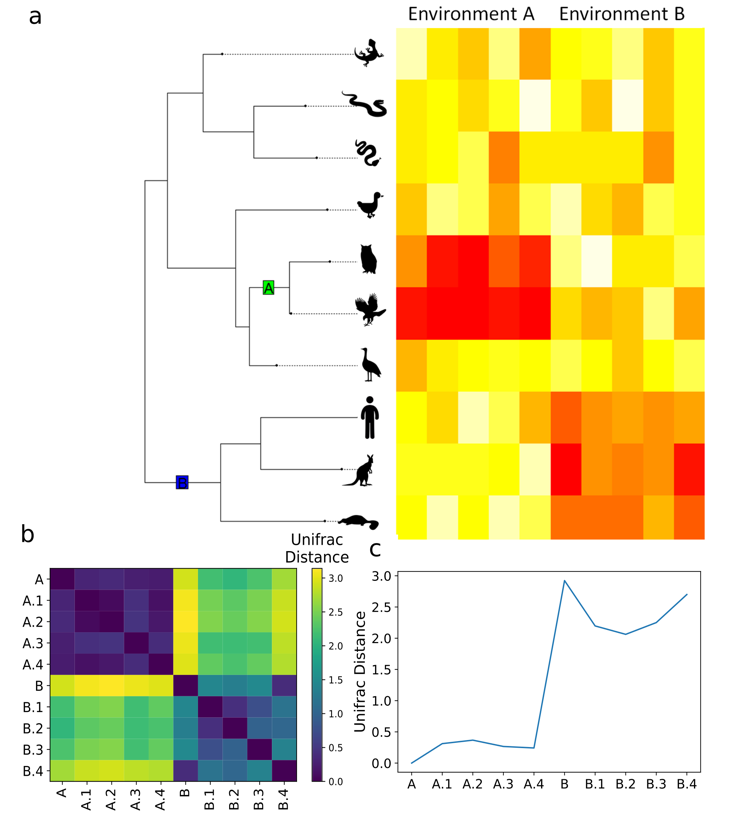
\includegraphics[width=0.7\textwidth]{ch1/figure3.png}
        \caption[A demonstration of how to interpret Unifrac distances.]
        {A demonstration of how to interpret Unifrac distances.(a) A heatmap of species abundances with red indicating high abundance and yellow indicating low abundance across different environments.  The evolutionary history is represented by the phylogenetic tree, and the main differences between Environment A and Environment B are being driven by the abundances in clade A and clade B. (b) While variables contain information for each sample, distances relate two samples. Plotted are the pairwise Unifrac distances between the samples; distances between samples from Environments A and samples from Environment B are larger compared to distances between samples from Environment A or distances between samples from Environment B. (c) The Unifrac distance between a sample from the Environment A to all other samples illustrates how distances can be useful for sample-site classification. Phylogeny-aware distances can relate to functional distances by capturing flow of abundances through edges along which traits arose.\index{SanDiego3}}
        \label{figa3}
\end{figure}

UniFrac distances are not the only possible phylogenetically-informed distances.  There have been a number of different distance metrics such as Sorensens' index, Rao's D and Rao's H that have been proposed alternative methods to incorporate evolutionary information \cite{Silverman2016-he}.  Furthermore, standard statistical techniques such linear regression can be augmented to penalize differences between close relatives\cite{phylogenetic_cca,purdom,fukuyama_perturbation}.The phylogeny is a scaffold for many variables, and can serve as the basis for many useful distance metrics. Which distance(s), of the possible distances, are of interest to a given microbiologist? \par
We suggest two main goals in the construction of phylogeny-aware distances: improving sample-site classification/visualization and providing meaningful interpretations of community differences. \par
If sample-site visualization is the goal of an experiment, a researcher may be inclined to search through a space of possible distances until finding one that looks the best, irrespective of the biological interpretability of the distance. Otherwise, searching too many distances risks dredging the data and presenting statistically significant patterns which were obtained by testing multiple candidates without proper corrections for multiple hypothesis tests performed. Correcting for such multiple tests will face the same challenges of unclear dependence among tests that arise in the analysis of multiple phylogenetic variables.
While many existing distances can successfully classify samples across a range of site categories and clinical variables, the biological implications of discovered differences are often unclear. Does a larger distance indicate greater difficulty in bioremediation of one community into another? Does a larger distance imply a larger difference in ecosystem function or patient morbidity? What follow-up experiments should one conduct to better understand the biochemical and microbiological causes of community differences, given a large UniFrac distance?\par
Construction of new phylogeny-aware distances and their use in modified statistical methods should consider the performance gains relative to existing methods and whether they provide a new interpretation of discovered differences. Careful justification of new distances can improve the biological interpretation of results. For instance, macroscopic ecologists debate how beta diversity can be used for conservation\cite{socolar_beta_diversity}. Such discussions can improve the interpretation of existing and newly developed phylogeny-aware distances and help researchers understand any implications of high or low distances between communities. In addition, a high quality tree is critical for revealing ecologically relevant patterns \cite{fast_unifrac}.  As with phylogenetic comparative methods and phylogenetic variables, phylogeny-aware distances benefit from explicit consideration of ecological and evolutionary models to aid the biological interpretation of their results.
\section{Challenges of phylogenetic analysis}
There are challenges to phylogenetically-structured data analysis, including \gls{hgt}, the choice of which gene tree to use, the sensitivity to errors in phylogenetic inference, and the explicit consideration of ecological and evolutionary models.\par
\gls{hgt} between microbial genomes complicates the evolutionary story of vertical transmission captured in a phylogenetic tree \cite{gogarten_hgt}. \gls{hgt} raises the question of which phylogeny to use and how informative the phylogeny is for the research question. For phylogenetic comparative methods, \gls{hgt} can lead to improper corrections and poorly calibrated statistical tests (illustrated in supplement). \gls{hgt} of a major trait driving variation in the data can reduce the appropriateness of the phylogenetic variables or distances being used.\par
It is favorable to choose gene families that are insensitive to \gls{hgt} for inferring phylogenies. Studies have evaluated the chance of \gls{hgt} based on functional and ecological features\cite{gogarten_hgt, complexity_hypothesis}, providing guidelines for this task. Perhaps there is no gene absolutely \gls{hgt}-free throughout the tree of life, including 16S \cite{kitahara_hgt}. Including multiple genes in phylogenetic inference can minimize the negative impact of \gls{hgt} \cite{phylophlan}, and reveal genes influenced by \gls{hgt} within the selected range of taxa\cite{purdom}. Computational tools are available for assessing the probability of putative \gls{hgt} events based on species/gene tree reconciliation\cite{Washburne2017-up}. Exploration of genomic context, sequence signature and atypical homology search results also help tracking \gls{hgt}s\cite{ravenhall_hgt}. \par
\gls{hgt} does not invalidate phylogeny-aware analyses of microbiome data. \gls{hgt} of functional traits could be hypothesized through phylogeny-aware analyses by strong effects with little phylogenetic signal \cite{lozupone_species_divergence}. If phylofactorization identifies an unusually large number of tips of the tree associated with antibiotic exposure, \gls{hgt} may be driving variation in the data and can be further tested by comparison of genomes among the phylogenetic factors identified. Nonetheless, \gls{hgt} requires consideration when analyzing phylogenetically-structured data. The sensitivity of many methods to the horizontal transfer of functional traits is currently understudied. The combination of \gls{hgt} and the existence of different phylogenies for each gene motivates careful justification of which genes to use to make phylogenies.
Finally, all methods face the challenge of being interpretable and advancing our knowledge of microbiological systems. To that end, new methods should explicitly consider ecological and evolutionary models for how traits evolve and drive patterns in the data. One study simulated trait evolution on a tree and compared \gls{pgls} with phylogenetic eigenvector regression methods\cite{phylogenetic_eigenvector}, which use eigenvectors from phylogenetic distance matrices as explanatory variables and do not correspond to a clear evolutionary model. The study found that \gls{pgls} produced more reliable and better-calibrated statistical results\cite{phylogenetic_eigenvector}. Considering evolutionary and population genetic models in method development promotes accurate understanding of the assumptions under which a phylogeny-aware analysis performs well and interpretation of findings in terms of the biological processes at play\cite{comparative_methods_fix}. \par
As more methods are developed, researchers should be aware of the tradeoffs between machine learning and human understanding: the former may produce more accurate predictions in the short term, whereas the latter produces theory that can generate more accurate and generalizable predictions in the long term.\par
\section{Discussion}
The common ancestry of microorganisms can be a source of confounding variation in our data, or a scaffolding on which we make inferences. There are many existing and emerging methods for analyzing microbiome datasets in light of evolution, and choosing the right method requires precise statements of the research question (Table 1).\par
First, decide which tree to use. Commonly, microbiome studies use the 16S tree for Bacteria and Archaea and the 18S tree for microbial eukaryotes, but there is a phylogeny for every gene and some questions are better analyzed with trees from other genes. The phylogeny obtained will be an estimate, and uncertainty in phylogenetic inference can translate to uncertainty in downstream phylogenetically-structured data analysis.\par
If the research question uses a trait as a response variable, the phylogeny may be a source of confounding variation. Phylogenetic comparative methods, such as \gls{pgls}, correct for dependence among traits one expects under null models of evolution along the tree.\par
If the research question is seeking historical trait values, or edges along which major trait differences arose, ancestral state construction is needed. If testing associations between imputed traits, researchers need to combine ancestral state reconstruction for imputation of missing traits with phylogenetic comparative methods which correct for confounding variation. \par
If the research question aims to simplify patterns of community composition, the phylogeny is a scaffolding that can be used to produce biologically informative variables and directions of change. The choice of variables should be made according to their ability to capture features in data, their statistical dependence, and their biological interpretation.\par
If the research question is to differentiate microbial samples, the phylogeny can define distances between samples. By re-defining distances, the phylogeny can be used to modify virtually any statistical method, but the choice of which distance to use should be based on the research goals of sample-site classification or biological interpretation of differences.\par
Phylogenetic analysis of microbiome data can allow researchers to categorize unclassified microorganisms, test evolutionary hypotheses about trait associations or traits driving habitat associations, and better understand how microbial communities differ and how they change over time, space, and treatments. There are several classes of methods for analyzing microbiome data “in light of evolution”. Careful consideration of the research question and the allowable ecological and evolutionary assumptions enables researchers to identify existing methods or produce novel methods that address their research question and produce novel, accurate, and biologically informative insights. The deluge of information about microbial sequences is producing phylogenetically-structured data which, given the right tools, can accelerate our understanding of microbial community structure and function.

\section{Acknowledgements}
J.T.M. was funded by NSF GRFP DGE-1144086. A.D.W. received support from Duke University Biology Department’s provision of start-up funds for D. Nemergut (deceased) and the Defense Advanced Research Projects Agency (DARPA) grant D16AP0013. This paper is published in the spirit of D. Nemergut’s contagious love of science.

Chapter 1, in full, is a reprint of the material as it appears in
``Methods for phylogenetic analysis of microbiome data''
Alex D. Washburne, James T. Morton, Jon Sanders, Daniel McDonald,
Qiyun Zhu, Angela M. Oliverio, Rob Knight  \emph{Nature Microbiology} 3, 2018. The dissertation author was the primary investigator and co-first author of this paper.


\chapter{Uncovering the horseshoe effect in microbial analyses}
The horseshoe effect is a phenomenon that has long intrigued ecologists.  Commonly thought to be an artifact of dimensionality reduction, multiple techniques were developed to unravel this phenomenon and simplify interpretation.  Here, we provide evidence that horseshoes arise as a consequence of distance metrics that saturate - a familiar concept in other fields but new to microbial ecology.   This saturation property loses information about community dissimilarity, simply because it cannot discriminate between samples that do not share any common features. The phenomenon illuminates niche differentiation in microbial communities and indicates species turnover along environmental gradients.  Here we propose a rationale to the observed horseshoe effect from multiple dimensionality reduction techniques applied to simulations, soil samples, and samples from postmortem mice.   An intuitive-depth understanding of this phenomenon allows for the targeting of niche differentiation patterns from high-level ordination plots.
\section{Introduction}
Ecological datasets, particularly those observed in microbiome studies, are typically sparse and high-dimensional, frustrating most conventional statistical techniques.  Many numerical ecology software packages make use of distance-based statistics by calculating the distance between ecological communities, to compare various ecosystems to each other over space and time.  One of the most common exploratory analysis techniques is ordination, where the distances between the communities are embedded into a Euclidean space, and then visualized via Principal Components Analysis (\gls{pca}) \cite{numerical_ecology}.  A widely used extension of this technique, where the distance metric can be varied, is called Principal Coordinates Analysis (\gls{pcoa}) \cite{numerical_ecology}.  \par
One phenomenon that commonly occurs in datasets containing ecological gradients is the horseshoe effect or Guttman effect \cite{global_patterns}.  This phenomenon is typified by a linear gradient that appears as a curve in ordination space. The horseshoe effect, or its relative the arch effect \cite{detrended_correspondence_analysis} (where the ends of the gradient do not attract each other along the first principal coordinate as they do in the horseshoe effect), is observed using multiple types of ordinations, including Principal Components Analysis, Principal Coordinates Analysis, Non-Metric Multidimensional Scaling, Correspondence Analysis, and many others \cite{numerical_ecology}.  In 1982, the prevailing view of the horseshoe effect arose, when it was described by Gauch as a mathematical artifact that obscures the underlying ecological gradient.  Soon thereafter, Detrending Correspondence Analysis \cite{detrended_correspondence_analysis} was invented to unbend the horseshoe using reciprocal averaging. Since then, detrending has become a commonly applied practice to ordinations in ecological datasets.   Although these detrending techniques appear to provide a more intuitive visualization, they have been criticized as providing a distorted perspective of the underlying data, relying on many parameter settings that cannot be chosen in a principled way, and obscuring true underlying patterns in the data \cite{trust_dca}.\par
\begin{figure}[H]
        \centering
        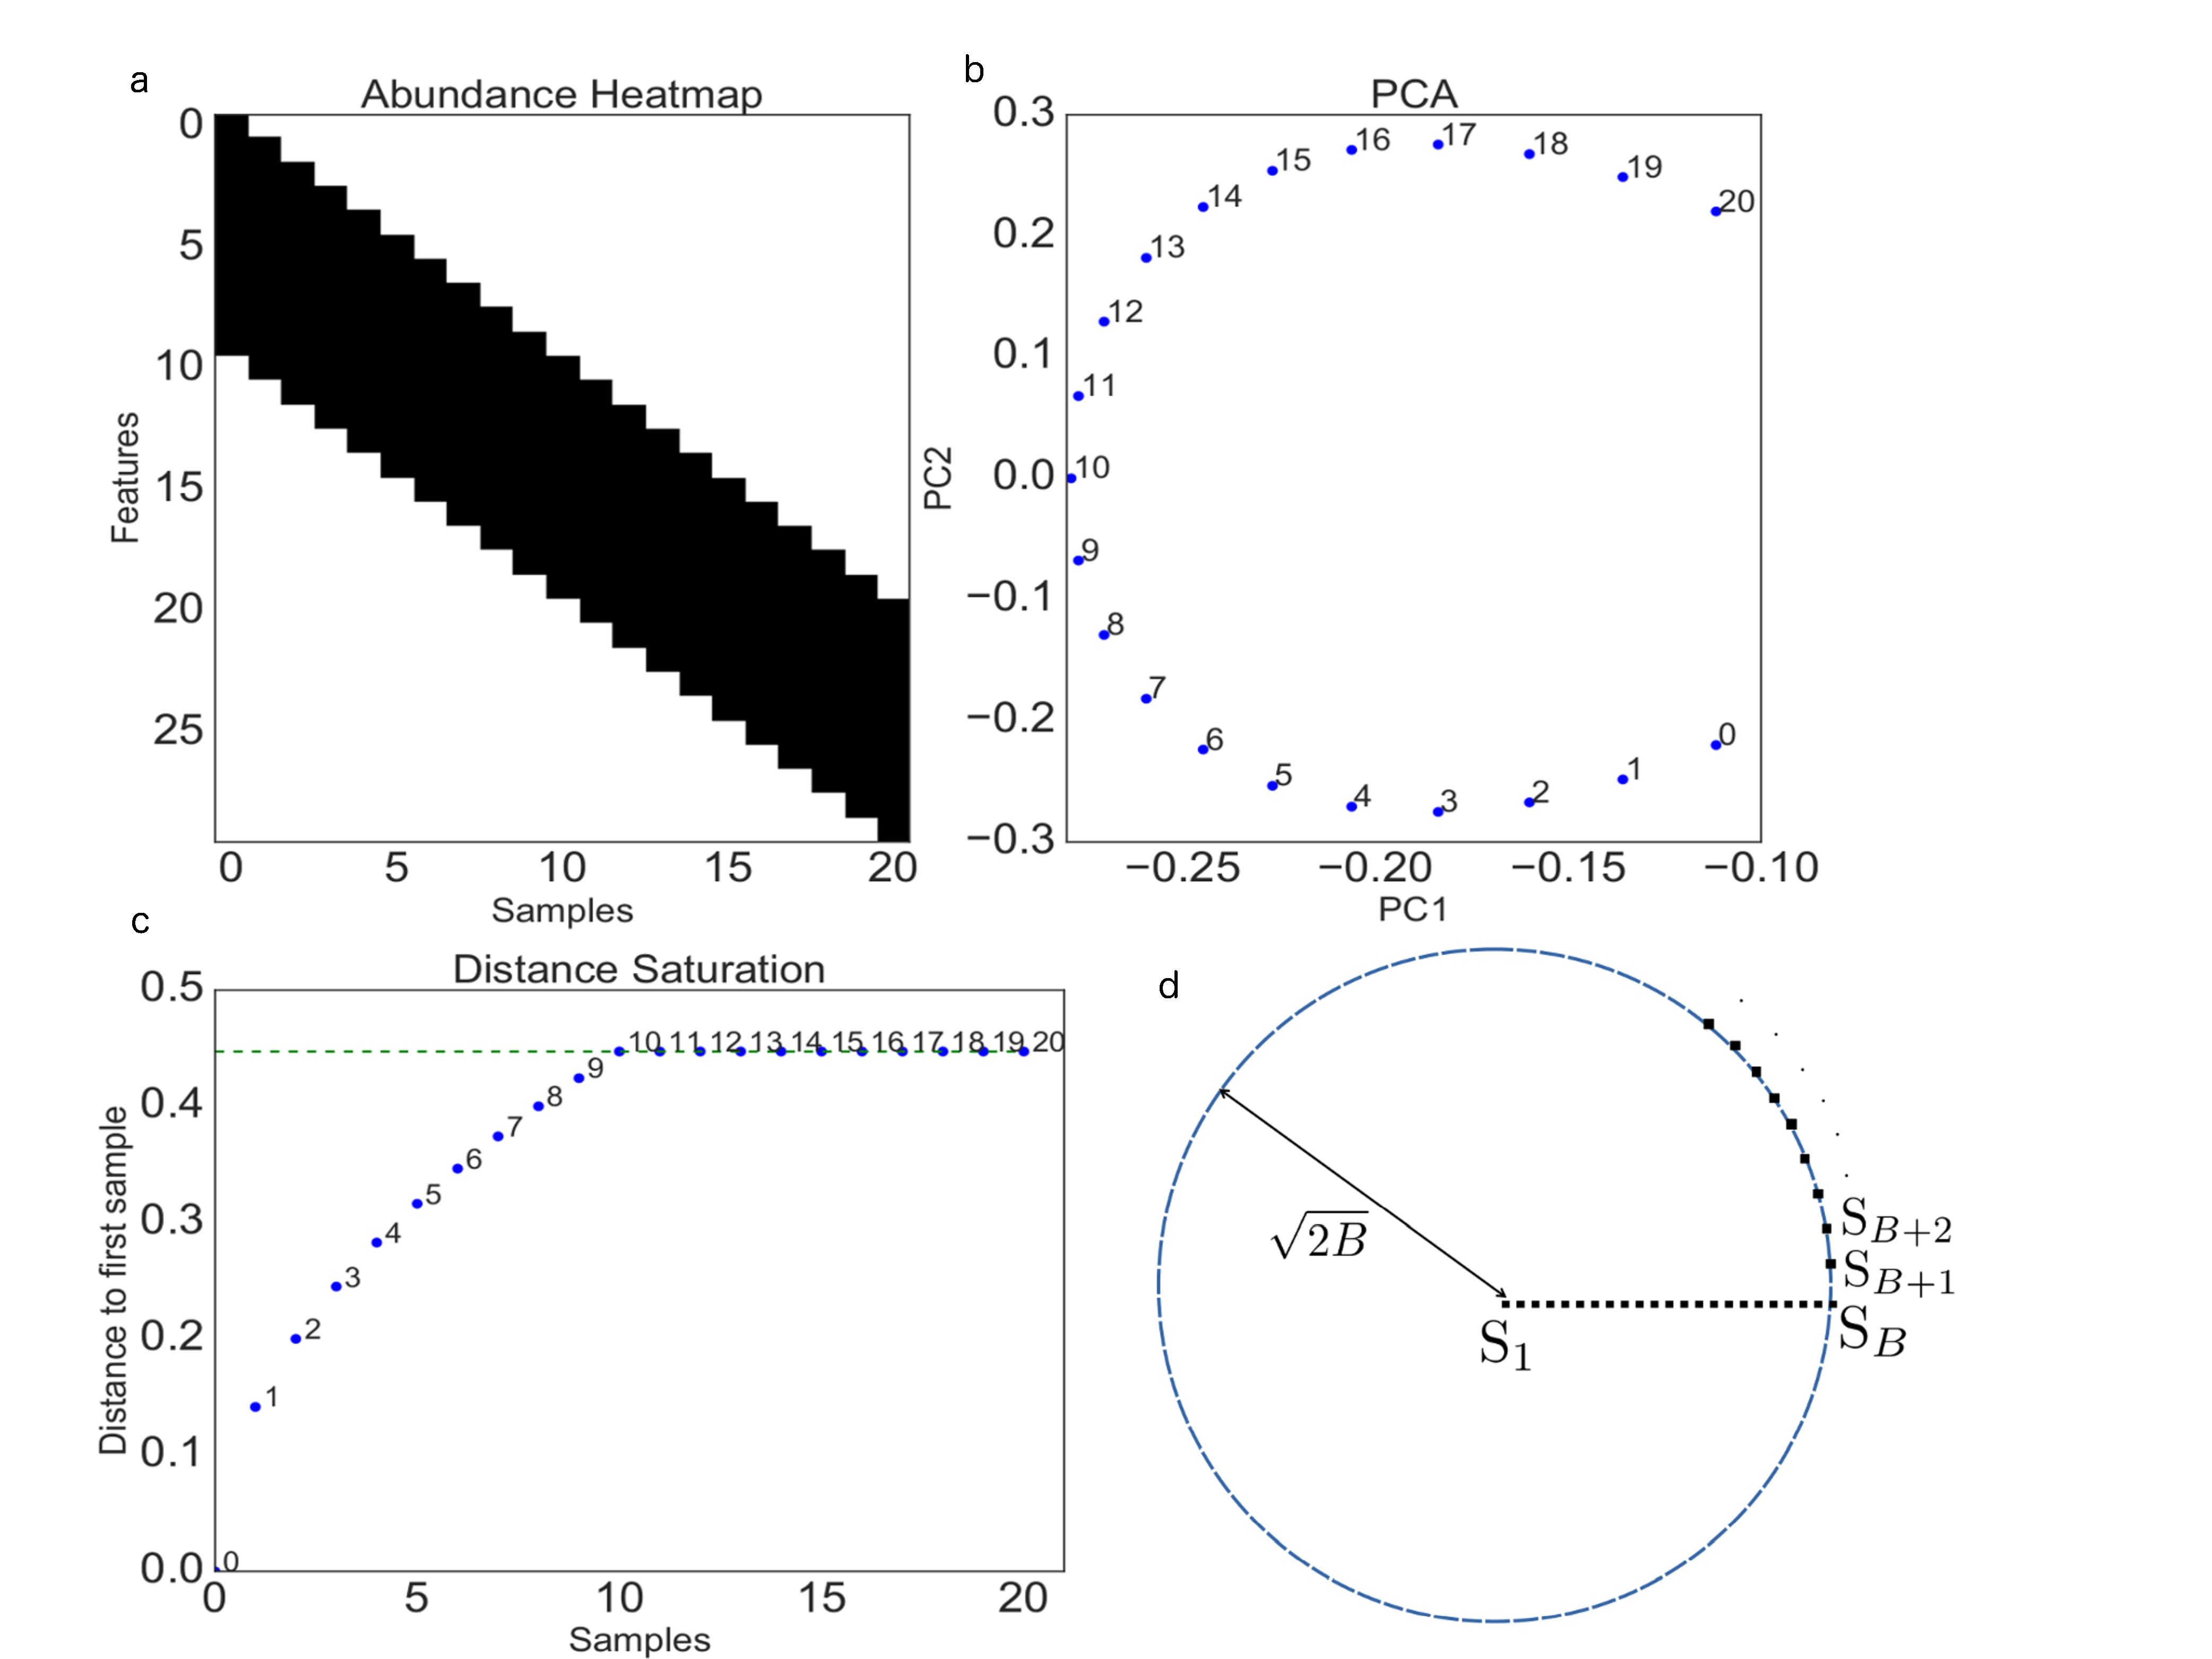
\includegraphics[width=1.1\textwidth]{ch2/Figure1.pdf}
        \caption[An explanation of the horseshoe effect arising from distance saturation.]
        {An explanation of the horseshoe effect arising from distance saturation. (a) A band table where the y axis encodes for individual \gls{otu}s and the x axis encodes for samples.  Blocks that are colored black have a value of 1/10 while blocks that are colored white have a value of 0.  (b) The first 2 components from a \gls{pca} of the band table, yielding the typical horseshoe shape.  (c) The Euclidean distance from the point 0 to all of the other points.  (d) An illustration of distance saturation property.\index{SanDiego6}}
        \label{figb1}
\end{figure}
From previous studies, it was shown that horseshoes can arise from band tables \cite{horseshoe_kernel, guttman_effect}.  These tables consist of highly dense, non-zero values along the diagonal of the table, and sparse values everywhere else.  This pattern can be apparent when the rows and columns are sorted in the proper order. Although the idea that band tables lead to horseshoes is not a new idea, it is commonly misunderstood how this concept applies to microbial analyses.  Here we provide some intuition behind the mathematical structure of horseshoes.\par
In Figure \ref{figb1}a, we show a simulated band table, where each vertical band is represented by a sample, and contains 10 non-zero values.  In typical microbiome datasets, these values could reflect \gls{otu} or species counts; for simplicity, here we will to refer to them as species counts, although this concept can also be generalized to multiple data types, such as gene counts, metabolite abundances.  Each sample in the table is shifted by 1 row, creating the band effect.  When \gls{pca} is applied directly to this table, the first 2 eigenvectors yield a horseshoe pattern (Figure \ref{figb1}b).  Here, the band table is parameterized with a band size of 10, since each sample has exactly 10 non-zero values.  \par
For close local points, the Euclidean distance grows linearly along the gradient (Figure \ref{figb1}c).  However, after a certain point, the distance completely saturates. This property has been previously noted with Euclidean distance \cite{detrended_correspondence_analysis}.  The overlap between the first sample in the band table, and sample 10 and beyond disappears, and the distance between these samples is maximized. This can yield unintuitive properties, sample 10 could be less dissimilar than sample 1 compared to sample 20.  For instance, sample 10 could represent a medium pH environment, sample 1 could represent an acidic low pH environment and sample 20 could represent a high pHbasic environment. Sample 1 is expected to be a substantially more different microbial community to Sample 20 than Sample 10.  The acidophiles found in Sample 1 are typically not found in basic environments. Sample 20 is expected to be more different to sample 1 than sample 10, since it contains very different microbes that thrive in high pH environments.  But as far as Euclidean distance is concerned, sample 10 is just as dissimilar to sample 1 as sample 20, just because there are no common bacteria shared between these samples.  It is apparent that the saturation property of Euclidean distance does not capture all of the information about community dissimilarity along a gradient, simply because it cannot discriminate between samples that do not share any common features.  Once the distance is saturated, all samples that do not overlap lie within a ball of radius B where B is the band size lie within a ball of radius where B is the band size and the first point is the center of the ball as shown in Figure \ref{figb1}d.\par
This saturation property has been suggested to give rise to horseshoes in previous studies in other fields \cite{horseshoe_kernel}, and is an unintuitive property that can confound ecological interpretations if not understood properly.  This property also restricts the possible trajectories of samples in the feature space, and gradients cannot be represented by linear trajectories in the real space (Supplemental proof 1). This means that communities in the original high dimensional space do not arrange into linear trajectories in the first place, and when projected to lower dimensions do not fall into linear trajectories.  These trajectories are what we refer to as horseshoes.  The horseshoe phenomenon is analogous to the familiar concept of saturation in molecular evolution, where two randomly evolving sequences saturate at 75\% DNA sequence identity (assuming equal nucleotide frequencies), even if infinite time has elapsed \cite{dna_saturation}. Consequently, distances that reflect a higher degree of molecular change need to be corrected for multiple substitutions in order to recover the molecular clock-like behavior obtained when comparing more similar sequences. This is why corrections according to models such as Jukes-Cantor or the Kimura 2-parameter model are required to obtain distances for reconstructing better phylogenetic trees. Analogous distance corrections are needed in microbial ecology for reconstructing better relationships among microbial communities \cite{evolutionary_distances}.\par
It is important to note that horseshoes do not only arise from \gls{pca}, but also arise in \gls{pcoa} with a variety of distance metrics.  Arch effects have plagued every multidimensional reduction technique we have applied to a wide range of microbial ecology datasets \cite{microbial_patterns}. In the following case studies, we'll show that these distance metrics also have the saturation property.  In addition, if a distance doesn't have this saturation property, there won't be an observed horseshoe artifact (Figure S1).\par
\section*{Case Study 1 - 88 Soils}
In this study, 88 soil samples were obtained from multiple locations across the United States having varying levels of pH \cite{soil_pyro}.  The V4 region of the 16S rRNA gene (16S) within each organism was amplified and sequenced using 454 pyrosequencing to obtain relative abundances of microbial taxa.  A matrix representing abundance values for each taxonomic unit per soil sample was used as input in correspondence analysis (\gls{ca}) \cite{correspondence_analysis}. The resulting ordination showed clear separation of the communities based on pH (Figure \ref{figb2}a), which led to the same conclusion that pH is a major driving factor in soil biogeography, i.e. pH has major impacts on the distribution of bacterial taxonomic units in soil \cite{soil_pyro}.  The \gls{ca} analysis in Figure \ref{figb2}a also shows the classic horseshoe shape.   Here we revisited this study, to better understand the horseshoe shape behind this dataset.\par
To test the effect of another commonly used distance metric on the sample distribution, we analyzed the same soil dataset applying Chi Squared distance (Figure \ref{figb2}b). Similar to what was observed with Euclidean distance, which was applied in the simulation, the Chi Squared distance increased sharply at pH 3 and 4, but began to saturate at pH of 5.  Also the band table similar to what we have observed in Figure \ref{figb2}a can be obtained when sorting.  Also, when the the \gls{otu} table was sorted by sample pH and the mean pH of the samples that the \gls{otu}s were observed in mean pH of the \gls{otu}s (Equation 12), the same band table pattern appeared as we show in Figure \ref{figb2}a.  While the diagonal isn't completely dense, there are more non-zero values compared to the corners of the heatmap. In line with the findings from the original study, this pattern is likely representative of niche differentiation of \gls{otu}s with respect to pH. The organisms that thrive in low pH environments tend not to exist in high pH environments and vice versa.  Low pH and high pH samples are shown in Figure \ref{figb2}c to have few overlapping species, a pattern not observed in the original study as membership was evaluated at coarser levels of taxonomic resolution\cite{soil_pyro}.\par
\begin{figure}[H]
        \centering
        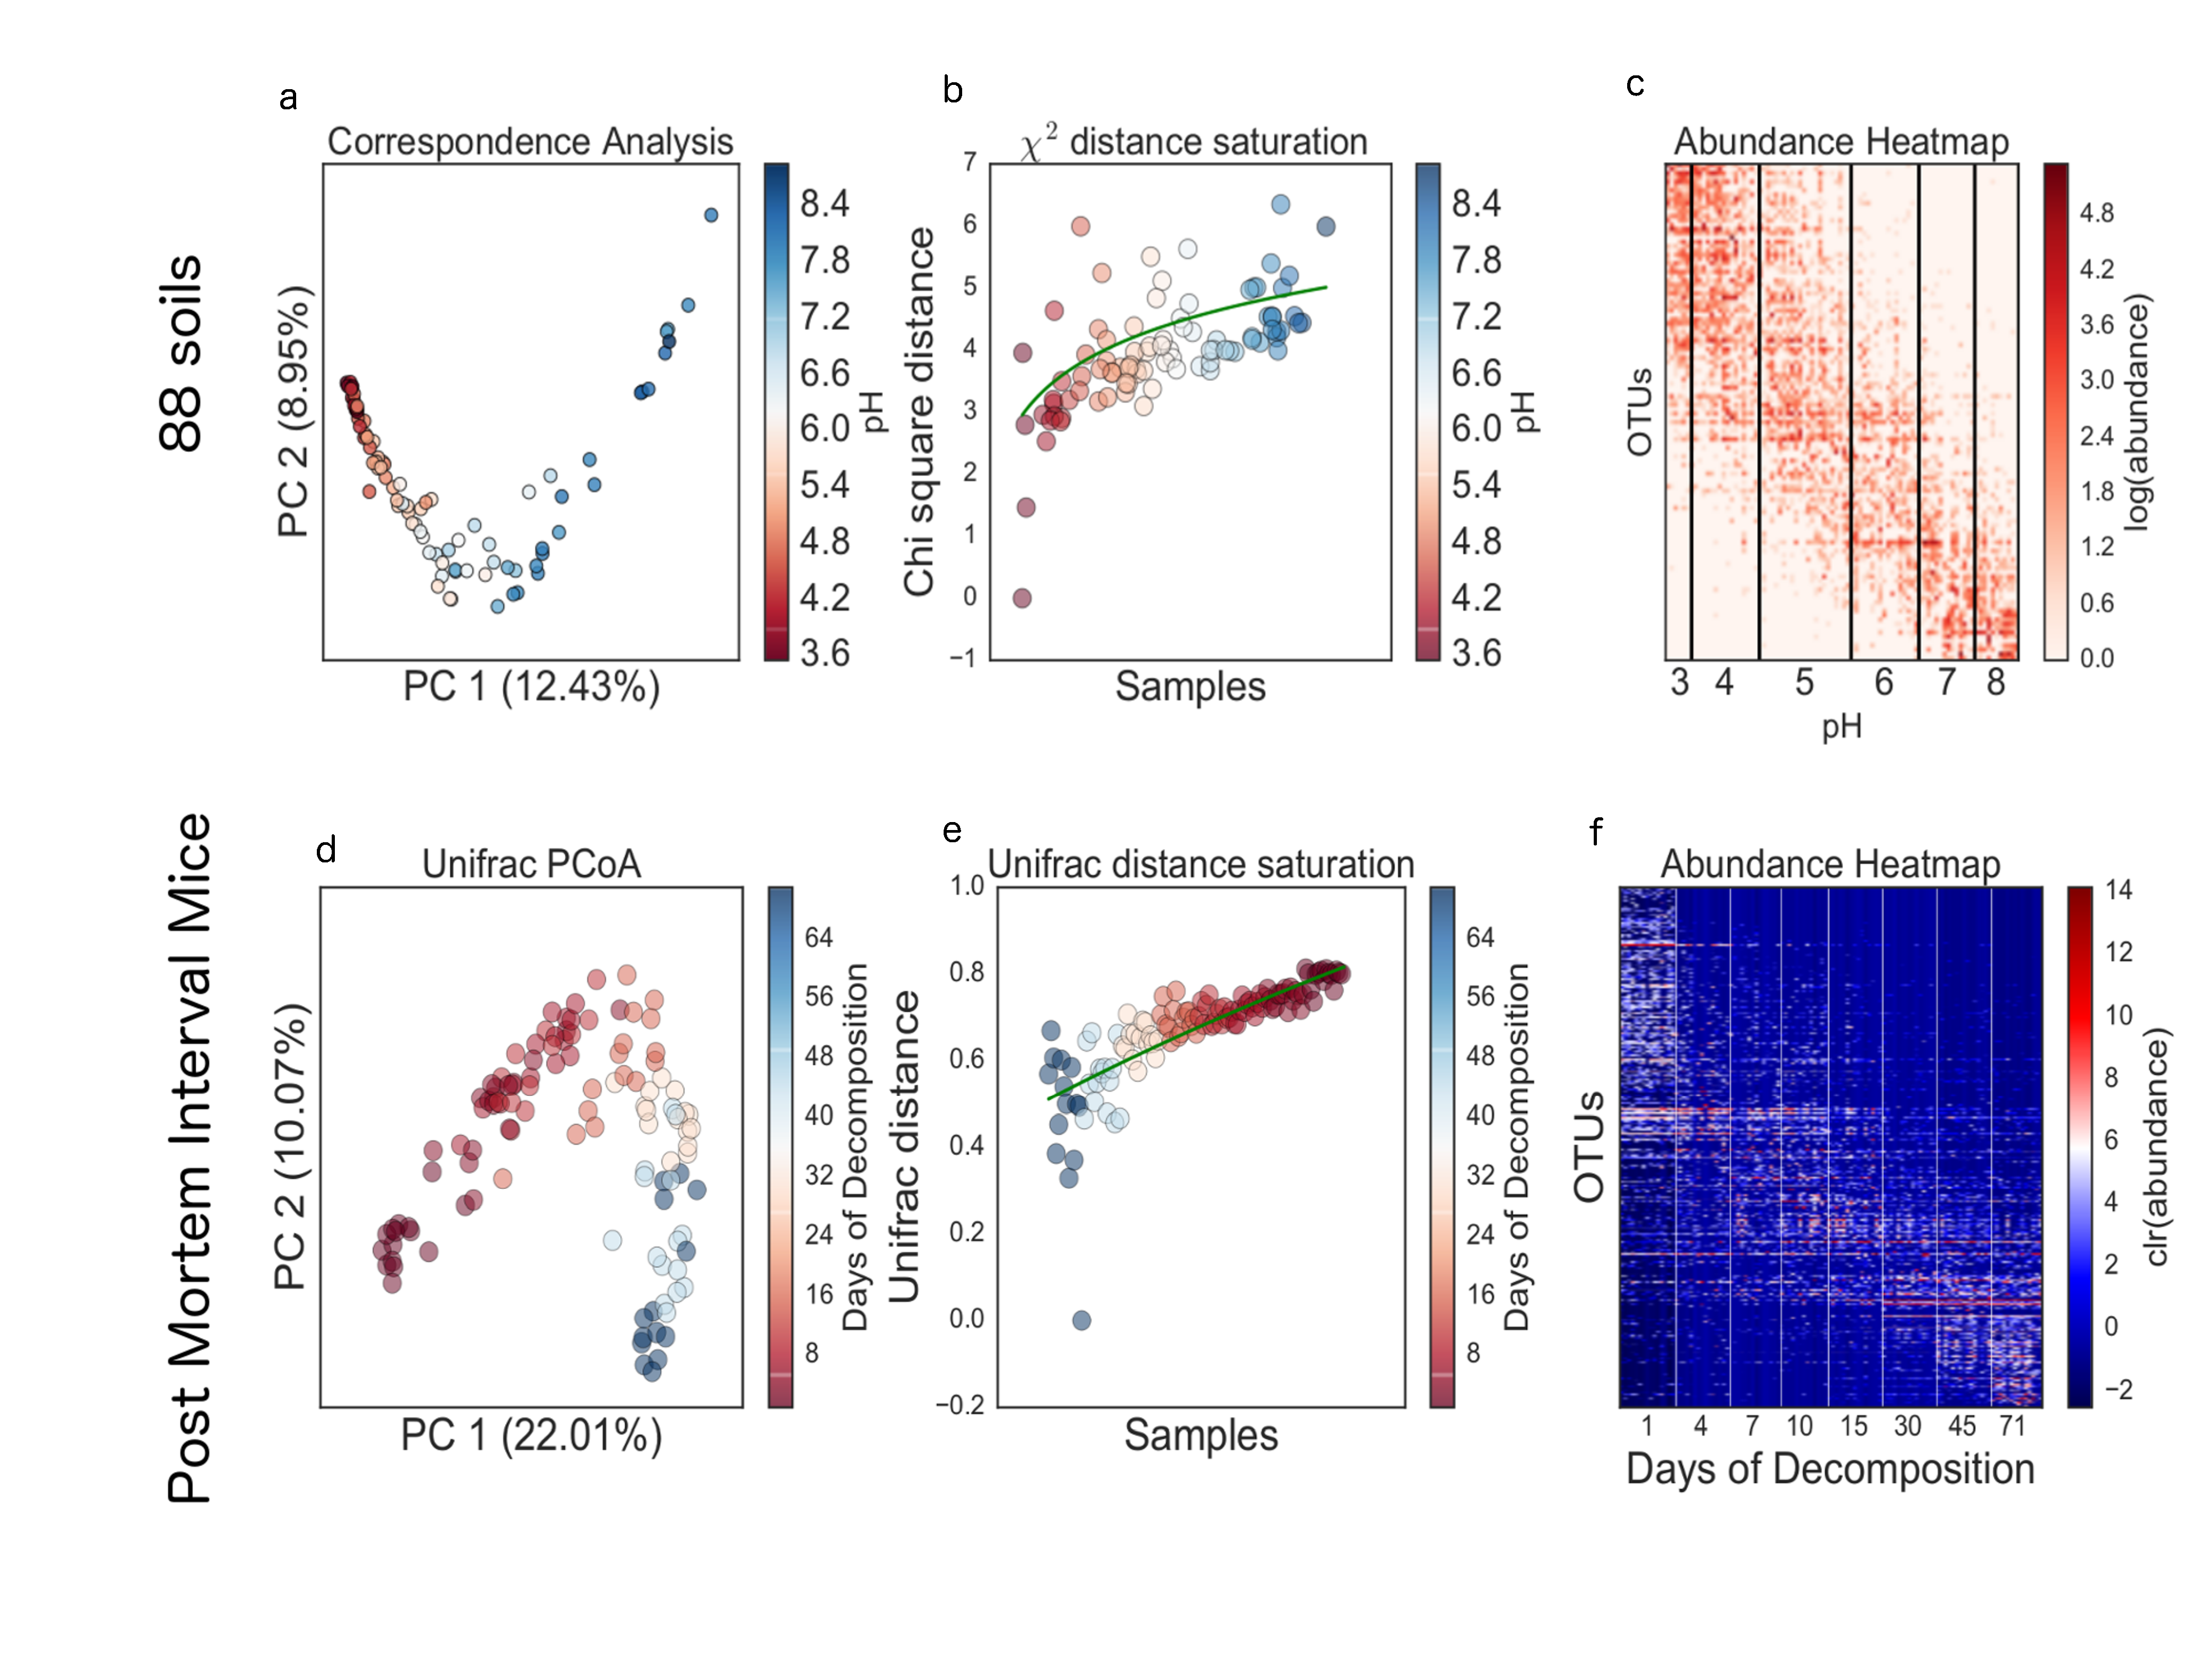
\includegraphics[width=1\textwidth]{ch2/Figure2.pdf}
        \caption[Two case studies show casing how horseshoes can appear in the context of
          soil microbial communities and post-mortem microbial communities.]
        {Two case studies show casing how horseshoes can appear in the context of soil microbial communities and post-mortem microbial communities. (a) Correspondence analysis of 88 soils.  (b) Distance saturation of chi-squared metric, plotting the chi squared distance of the first sample versus all of the other samples. (c) Heatmap of log transformed \gls{otu} counts from the 88 soils with the samples sorted by pH and the \gls{otu}s sorted by mean pH.  (d) Principal Coordinates Analysis of unweighted UniFrac distance.  (e) UniFrac distance of a samples from the last time point versus all of the samples. (f) Heatmap of centred log ratio transformed (Equation 2) \gls{otu} counts sorted by harvest days.\index{SanDiego8}}
        \label{figb2}
\end{figure}
\section*{Case Study 2 - Post Mortem Mice Study}
In this study, 120 mice were sacrificed and allowed to decompose on soil. Mice were destructively sampled over approximately 8 weeks\cite{mammalian_corpse}. 16S sequencing libraries were generated from total DNA extracted from swabs of the skin on the head, and relative abundance values were calculated for each bacterial \gls{otu}. A relative abundance matrix was generated for each library and used as input in \gls{pca}. This analysis generated a clear horseshoe (Figure \ref{figb2}d) using unweighted UniFrac distance \cite{soil_pyro}, with a gradient with respect to the time since death, possibly reflecting a changing skin microbiome during decomposition of the mouse carcass. When the samples were sorted by time since death using a similar strategy as noted above, a band table emerges (Figure \ref{figb2}f). Also, the unweighted UniFrac distance analysis appears to have the same saturation property as observed previously with Euclidean distance and Chi-squared distance.  It is important to note that highest possible UniFrac distance is 1, suggesting that this distance metric can also be saturated.  In Figure \ref{figb2}e, while the distance hasn't completely saturated, these distances are quickly approaching the theoretical maximal UniFrac distance. \par
The striking changes in microbial communities during decomposition are associated with dramatic environmental biochemical changes, including increased pH, ammonia, and total nitrogen, all measured in soil beneath the mice. Correspondingly, microbial communities are predicted to increase in gene abundance of important nitrogen cycling pathways such as amino acid degradation (e.g. glutamate dehydrogenase, lysine decarboxylase, ornithine decarboxylase) and nitrate reduction (e.g. nitrate and nitrite reductase). Bacterial taxa in the families Chromatiaceae (\gls{otu} 46026, 4482362) and Rhizobiaceae (\gls{otu} 4301099) are involved in nitrogen metabolism and become abundant as mouse bodies progress through the stages of decomposition (e.g. Fresh, Active Decay, Advanced Decay).  As shown in Figure S1, all of these \gls{otu}s peak at specific timepoints. The two Chromatiaceae \gls{otu}s peak during Active Decay (bloating and purge of fluids) at 15 days of decomposition. The Rhizobiaceae \gls{otu} peaks during Advanced Decay (sinking and sagging flesh) at 30 days of decomposition and when pH, ammonia, and total nitrogen were measured at their highest levels \cite{mammalian_corpse}.\par
To further validate if saturation leads to horseshoes, a new distance metric \gls{embad} (Earth Mover Band Aware Distance) was engineered to be non-saturating as a proof of concept (Supplemental Methods).  This distance metric uses prior knowledge about the ordering of the band table, and is determined by calculating the flow between two samples. As shown in Figure S1a, sample 1 and sample 2 each have 4 species proportions.  To calculate the distance between sample 1 and sample 2, the probability mass of species 1 and species 2 needs to be shuffled over to species 3 and species 4.  This concept is analogous to computing maximum flow along a pipe, and can be calculated using Earth Mover's distance \cite{emd, unifrac_emd, unifrac}.\par
For the 88 soils (Figure S1b), the \gls{embad} was applied to the pH sorted table. Therefore, even if two samples are not overlapping, samples closer together will have a smaller distance than samples farther apart in the gradient.  This is because the distance is defined to be not saturating and explicitly accounts for the pH gradient.  The same strategy was employed for the postmortem interval mice (Figure S1c), sorting the table by decomposition days. The \gls{pcoa} plots resulting from these applications of \gls{embad} suggest that a non-saturating distance metric could remove the horseshoe effect from lower dimensional projections of these abundances.  This provides further evidence that this saturation property could explain the the horseshoe phenomenon.\par
For the 88 soils study a \gls{permanova} test investigating the difference between soils with a pH less than 3, and soils with a pH greater than 8.  With the \gls{embad} distance metric the \gls{permanova} gave a pseudo F-statistic of 650.5 and a p-value of 0.0003, which has a much larger effect size compared to the original Chi-squared distance metric with a pseudo F-statistic of 3.8 and a p-value of 0.0004 with 9999 permutations.  A similar trend was observed in the post mortem interval mice study when testing the first decomposition day to the last decomposition day using \gls{permanova}.  The \gls{embad} distance metric had a pseudo F-statistic of 439.8 and a p-value of 0.0001 with 9999 permutations, which has a larger effect size than the Unifrac distance metric, which had a pseudo F-statistic of 25.5 and a p-value of 0.0001. This method is relieved from misinterpretations of data due to horseshoes and arches and facilitates the interpretation of taxonomic units along biologically significant gradients that reflect the selective pressure of these factors on the distribution of microbes.  \par
In light of the benefits of engineering a non-saturating distance metric, the \gls{embad} distance metric requires the gradient to be known a priori.  Generalizing this approach in the absence of known gradients is a difficult problem would require an exhaustive using known algorithms.  Specifically, this problem falls under the category of NP-hard problems (Supplemental Proof 2).  In the 88 soils study and the post mortem mice study, we were fortunate to be able to infer the underlying band table with known metadata.  \par
The band patterns we observe here are probably very common in ecology studies investigating species distribution patterns across spatial or temporal gradients. The pattern confirms microbial ecological fundamentals, i.e. bacteria have acquired unique adaptations to the environment and occupy either a broad range or very specific niches. In our case studies of the 88 soils - and the postmortem mice we confirmed that by using a band table pattern analysis approach, bacterial species show different adaptations to pH and bacterial diversity changes over time during decomposition of mice carcasses. The band pattern approach we apply here represents an additional method to visualize differences between microbial communities.\par
Based on our observations here, the horseshoe effect appears in dimensionality reduction techniques due to the saturation property of distance metrics.  While we have only tested a few distance metrics, it is suspected that a vast majority of these distance metrics exhibit the same property, which would also explain why horseshoes are encountered so frequently across many different fields. The saturation property has also been observed in multiple other fields, and other studies from different disciplines have come to similar conclusions \cite{horseshoe_kernel}. In addition, multiple techniques such as self organizing maps \cite{self_organizing_maps} and local linear embedding \cite{local_linear_embedding} attempt to avoid this saturation phenomenon by focusing on distances of nearby points.\par
In spite of the saturation property of distance metrics, identifying horseshoes is still highly useful for identifying patterns concerning niche differentiation.   Properly understanding this phenomenon will motivate the use and development of algorithms such as biclustering \cite{biclustering} to uncover underlying band patterns.  These insights will in effect allow us to identify microbial niches along different environmental conditions.\par
\section{Materials and Methods}
All analyses can be found below on github \\
\url{https://github.com/knightlab-analyses/horseshoe-analyses}.
The mean gradient used for the 2 case studies was calculated as follows.
\begin{equation}
        \overline{g}_{x}=\sum_{i=1}^{N}g_{i}\frac{x_{i}}{\sum_{j=1}^{D}x_{j}}
\end{equation}
Where $x_{i}$ is the proportion of \gls{otu} \textit{x} in sample \textit{i} , $\overline{g}_{x}$ is the mean gradient of \gls{otu} \textit{x}, and $g_{i}$  is the sample gradient at sample i. This calculation can be found in the gneiss package under the function \textbf{mean\_niche\_estimator}. The function used to sort the tables in Figure \ref{figaS1}c used \textbf{niche\_sort}. In the 88 soils study, the table was sorted by sample pH and the mean pH of the samples that the organisms were observed in. In the post mortem mice study, the table was sorted by the days of decomposition and the mean day of the samples of that the organisms were observed in.\par
The heatmap in Figure \ref{figaS2}f and the abundances in Figure S2 were normalized using the centre log ratio \gls{clr} transformation given by the following equation.
\begin{equation}
        clr(x)=\left [ \log \frac{x_{1}}{g(x)},...,\log \frac{x_{D}}{g(x)} \right ]=\log x-\overline{\log x}
\end{equation}
Where $g(x)=\sqrt[n]{\prod_{i=0}^{n}x_{i}}$ is the geometric mean and $\overline{\log x}=\log g(x)=\frac{1}{n}\sum_{i=0}^{n}\log x$ is the average of the log transformed values.  A pseudocount of 1 is added to all of the counts to prevent logarithms of zero occurring. \par
Analyses were performed using Scipy, Numpy, Matplotlib, Seaborn, Scikit-bio and Gneiss.
\section{Acknowledgements}
We thank Noah Fierer for his input on the analysis of the 88 soil samples and Dan Knights for discussion on the \gls{embad} metric. We also acknowledge Amnon Amir and Tomasz Kosciolek for their insights into the horseshoe effect. Finally, we thank Susan Holmes for her insights on previous work understanding the horseshoe effect.

J.T.M. was funded by NSF GRFP DGE-1144086. J.L.M. and R.K. were funded by the Office of Justice Programs National Institute of Justice (award NIJ-2011-DN-BX-K533).

Chapter 2, in full, is a reprint of the material as it appears in
``Uncovering the Horseshoe Effect in Microbial Analyses''
James T. Morton, Liam Toran, Anna Edlund, Jessica L. Metcalf,
Christian Lauber, Rob Knight \emph{mSystems}, 2, 2017.  The dissertation author was the primary investigator and first author of this paper.

\chapter{Balance trees reveal microbial niche differentiation}
Advances in sequencing technologies have enabled novel insights into microbial niche differentiation, from analyzing environmental samples, to understanding human diseases and informing dietary studies.  However, identifying the microbial taxa that differentiate these samples can be challenging. These issues stem from the compositional nature of 16S \gls{rrna} gene data (or, more generally, taxon or functional gene data), which changes in the relative abundance of one taxon influence the apparent abundance of the others.  Here we acknowledge that inferring properties of individual bacteria is a difficult problem, and instead introduce the concept of balances to infer meaningful properties of sub-communities, rather than properties of individual species.  We show that balances can yield insights about niche differentiation across multiple microbial environments including soil environments and lung sputum. These techniques have the potential to reshape how we carry out future ecological analyses aimed at revealing differences in relative taxonomic abundance across different samples.
\section{Introduction}
The ultimate goal for many microbial ecologists is to fully characterize niches of microbial organisms and understand interactions among taxa.  An understanding of how microbial communities are affected by environmental conditions could yield insights into microbial interactions and their role in macro-ecological processes, such as nitrogen fixation \cite{nitrogen_fixation} and acidification \cite{acidification}. But despite the extraordinary increase in available data brought about by advances in DNA sequencing, characterizing niche differentiation in microbes remains an outstanding problem, partly due to the difficulty of correctly interpreting compositional data.  Broadly speaking, a compositional dataset is represented by relative abundances, or proportions that individually carry no meaning on the absolute abundance of a specific feature (i.e. 20\% of 100 and 20\% of 10,000 are very different absolute abundances).  The constraints associated with compositional data are well known, but unfortunately often neglected in microbial ecology, leading to conflicting interpretations and irreproducible analyses \cite{gloor_epi, fodor_coda} .\par
\begin{figure}[H]
        \centering
        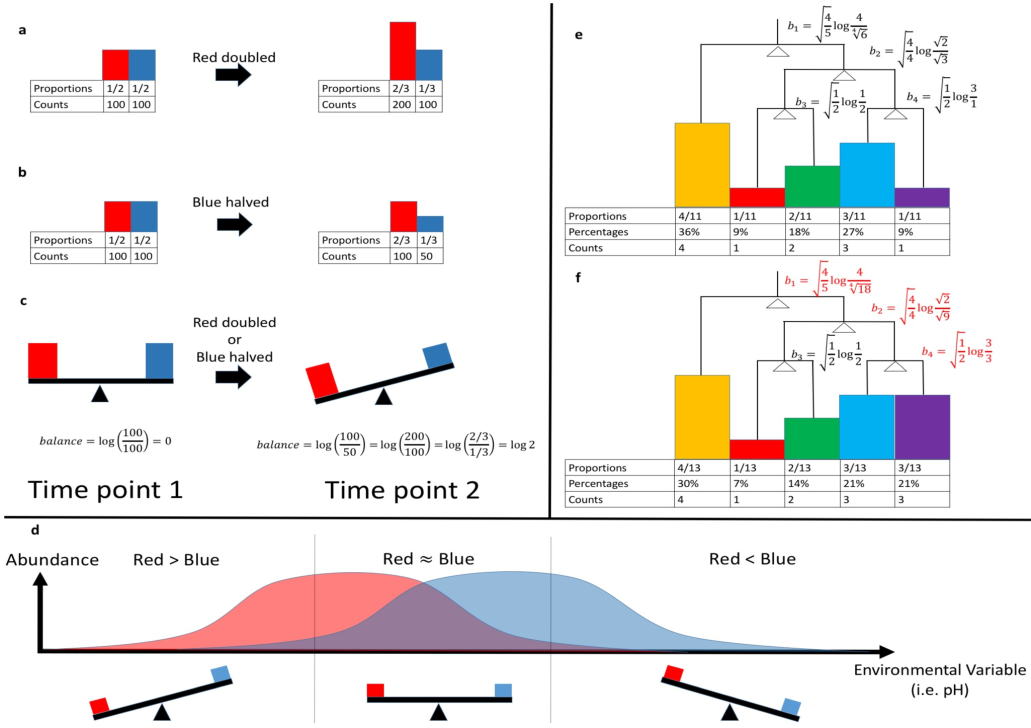
\includegraphics[width=1\textwidth]{ch3/Figure1.pdf}
        \caption[An explanation of balances and how to interpret them.]
        {An explanation of balances and how to interpret them. (a, b) A hypothetical scenario where 2 samples of 2 proportions could explain two different scenarios in the environment.  The balance between these 2 proportions is consistent for both scenarios.  (c) The balance of Red and Blue species abundances.  (d) balances of Red and Blue individuals across an environmental variable.  (e, f) The comparison of proportions and balances of two environments in the scenario where the Purple Orange population (i.e. the most right bin) triples. The balances were calculated using the groupings specified by the tree.\index{SanDiego8}}
        \label{figc1}
\end{figure}
We illustrate an example of this problem in Figure \ref{figc1}.  In this scenario, there are two species, “Red” and “Blue”. At the first time point, there are 100 Red individuals and 100 Blue individuals (Figure \ref{figc1}a). At the next time point, the number of Red individuals doubles, yielding 200 Red individuals, and the proportion of Red and Blue individuals becomes 2/3 and 1/3, respectively (Figure \ref{figc1}b). Suppose that we do not know the true total number of individuals in the given environment, and can only make inferences about the observed proportions -- a common scenario in microbial ecology, where absolute quantification is rarely performed.  In Figure \ref{figc1}b, the community has the exact same proportions at Time 1 and Time 2 as Figure \ref{figc1}a; however, instead of the Red individuals doubling at the second time point, the number of Blue individuals is halved (Figure \ref{figc1}c).\par
This is the problem with compositionality -- based on proportions alone, it is impossible to determine whether the growth or decline of any individual species has truly occurred \cite{Lovell_David_Muller_Warren_Taylor_Jennifer_Zwart_Alec_Helliwell2010-na}, and the inherent feature of one change in abundance driving abundance changes in another species violates assumptions of independence.  Analyses that rely on such assumptions, as many statistical approaches do, are thus prone to misinterpretation. For example, traditional correlation metrics such as Pearson and Spearman can be misleading when estimating microbe-microbe correlations \cite{sparcc, proportionality, spiec_easi, weiss_normalization}.  As a result, it becomes a major challenge to specify types of interactions between microbes, such as parasitism, competition, predation or mutualism, as shown in correlations studies in oral, fecal and vaginal samples from the Human Microbiome Project \cite{faust_microbial_interactions} \cite{sparcc}.  Even more advanced correlation-detection techniques such as SparCC \cite{sparcc} and SPIEC-EASI \cite{spiec_easi}, struggle with this, and typically require additional assumptions such as sparse \gls{otu} correlations (i.e. few \gls{otu}s are actually correlated with each other).  Furthermore, interpreting the resulting network is a major challenge, making it difficult to differentiate between true ecological relationships and random processes \cite{faust_microbial_interactions}.\par
The compositionality problem is also problematic for statistically detecting differentially abundant microbes across environments or between groups — consequently, it is a major barrier to reliably drawing conclusions about realized microbial niches using community sequencing data. Conventional statistical tools such as t-test and Mann-Whitney can incorrectly identify nearly 100\% of the taxa present in samples to be significantly different across environments (Figure S1), and univariate tests such as t-tests and ZIG \cite{metagenomeSeq} have been shown to mislabel microbes as significantly different across sample groups up to 60\% of the time \cite{ancom}. More advanced tools for differential abundance detection such as (\gls{ancom}) \cite{ancom}, are typically designed to control for false-positives and reliably detect differentially abundant species, but require multiple assumptions (i.e. the number of changing microbes across environments is small) and may require complex parameter tuning. To help overcome these issues of compositionality, we explore using the concept of balances, by moving away from inferring changes of individual species to instead inferring changes of microbial sub-communities to study niche differentiation of microbial communities.\par
\section{Concept}
Balances were first introduced as an exploratory technique in geology \cite{groups_of_parts, coda_dendrogram}. Fundamentally, they overcome the prhoblem of inferring changes in abundance from compositional data by sidestepping it, and instead inferring changes in the balance between particular subsets of the community. To understand the concept, let us revisit the scenario in Figure \ref{figc1}a and \ref{figc1}b.  Instead of examining proportion changes, we can investigate the balance between Red and Blue individuals by taking the log ratio of Red and Blue counts (Figure \ref{figc1}c).  By looking at the balance of these two species, we avoid incorrectly attempting to infer absolute increases or decreases in their abundances.  Instead, we can focus on the balance of the Red and Blue individuals, and directly infer the transition of dominance between these species.\par
These balances can also be useful for understanding species distributions across different covariates — a key proximate goal of microbial ecology, and one that is both crucial to the larger goal of niche characterization and heavily impacted by problems inherent in compositionality.  In Figure \ref{figc1}d, the Red individuals tend to exist in the low pH end of the spectrum, while the Blue individuals tend to exist in the high pH end of the spectrum.  A single balance can capture information about the transition from a high relative abundance of Red individuals in low pH environments to a high relative abundance of Blue individuals in high pH environments.  In low pH environments, the balance is positive, since there are proportionally more Red individuals than Blue individuals.  When the Red and Blue individuals are present in roughly equal proportions, the balance is roughly zero, representing a turning point, transitioning from a Red dominated community to a Blue dominated community.  As the pH increases, the balances become increasingly negative, since there are more Blue individuals than Red individuals. This balance effectively encodes for the niche separation of Red and Blue individuals across the pH gradient. \par
This idea of balances can be extended to multiple dimensions — and more than two taxa — using bifurcating trees.  A bifurcating tree can be built relating microbial taxa to each other using any criterion, and balances can be calculated on the internal nodes of the tree from the geometric means of the corresponding sub-trees. The appropriate criterion to build a tree depends on the question at hand.  A phylogenetic tree could be used to investigate evolutionary relationships of microbes \cite{Silverman2018-ql, Washburne2017-up}, or hierarchical clustering of environmental variables could be used to explore environmental niches of microbes.  To gain more intuition about this, consider Figure \ref{figc1}e, in which there are five species and 11 individuals. The four balances (internal nodes in the tree) are calculated by taking the log ratio of geometric means of sub-trees, also known as the isometric log ratio (\gls{ilr}) transform.  The full equation to calculate balances for a single sample is as follows,
\begin{equation}
b_{i}=\sqrt{\frac{\left| i_{L}\right| \left| i_{R}\right|}{\left| i_{L}\right|+ \left| i_{R}\right|}}log \frac{g(i_{L})}{g(i_{R})}
\end{equation}
where $b_{i}$ is the balance of the at internal node i ,  $i_{L}$, is the set of all species proportions contained in the left sub-tree at internal node i, $i_{R}$,  is the set of all species proportions contained in the right subtree at the internal node  i, g(x),  is the geometric mean of all of the proportions contained in vector $x$, $ \left| i_{R}\right|$,  is the number of species contained in  $i_{R}$ , and  $ \left| i_{L}\right|$ is the number of species contained in $ i_{L}$ (see Materials and Materials for more details). Following this equation, in Figure \ref{figc1}f  $b_{1}$ is calculated by taking the log ratio of the Yellow species and the geometric mean of the Red, Green, Blue, and Purple species.  \par
 It's also important to note that the some of the balances don't impact each other.  For instance, the changes in b4 do not impact the changes in b3, just because these balances don't share any common tips.  This is crucial, because this property allows us to ignore some of the variance of the balances towards the tips of the tree, and focus on the balances closer to the root of the tree.  These balances toward the root of tree capture the most information, since they contain a significant proportion of tree tips.  As a result, these high level balances have the potential to explain large shifts in these microbial communities.  The choice of the tree can allow for analysts to embed prior knowledge into the structure of the tree to test for these large community shifts.\par
 Here, we will discuss two studies from which novel insights were gained from this application.  While there are many compositionally aware tools available that are designed to identify microbial interactions and abundance fluctuations, we will refrain from benchmarking balances against these tools, as balances answer a conceptually different question.  These analyses are not restricted to analyzing ratios of individual \gls{otu}s and can be easily extended to analyze ratios of subcommunities.  \par
\section{ Results}
 \subsection{Case Study \#1 – Balances of pH-driven subcommunities in soils}
 In this study \cite{soil_pyro}, 88 soil samples were collected from North and South America, along with many edaphic measurements.  The study reported that there was a strong correlation between pH and species richness, suggesting that pH was a strong driver behind fluctuations in soil microbial communities. Acidobacteria were found to be negatively correlated with pH and Actinobacteria and Bacteroidetes to be positively correlated with pH, while Alpha/Beta/Gammaproteobacteria were not correlated with pH at all.  These correlation analyses are a little misleading, since the pH was correlated with each of the phyla independently.  The problem with this approach is that it does not account for all of the other phyla: similar to the argument made in Figure \ref{figc1}b, the change in a single phylum could also be explained by correlated changes in all of the other phyla.  Here, the negative correlation between Acidobacteria and pH could also be caused by the positive correlation between Bacteroidetes and pH.  Additionally, we cannot determine whether the Alpha/Beta/Gammaproteobacteria are correlated with pH or not.  Another possibility is that these three phyla could be positively correlated with pH, while Acidobacteria is not correlated with pH.  However, Bacteroidetes may be so strongly correlated with pH that Acidobacteria appears to be negatively correlated with pH, and the other three phyla not correlated with pH at all.  This scenario is one of the infinite possible underlying relationships that can explain these observed correlations. \par
 \begin{figure}[H]
        \centering
        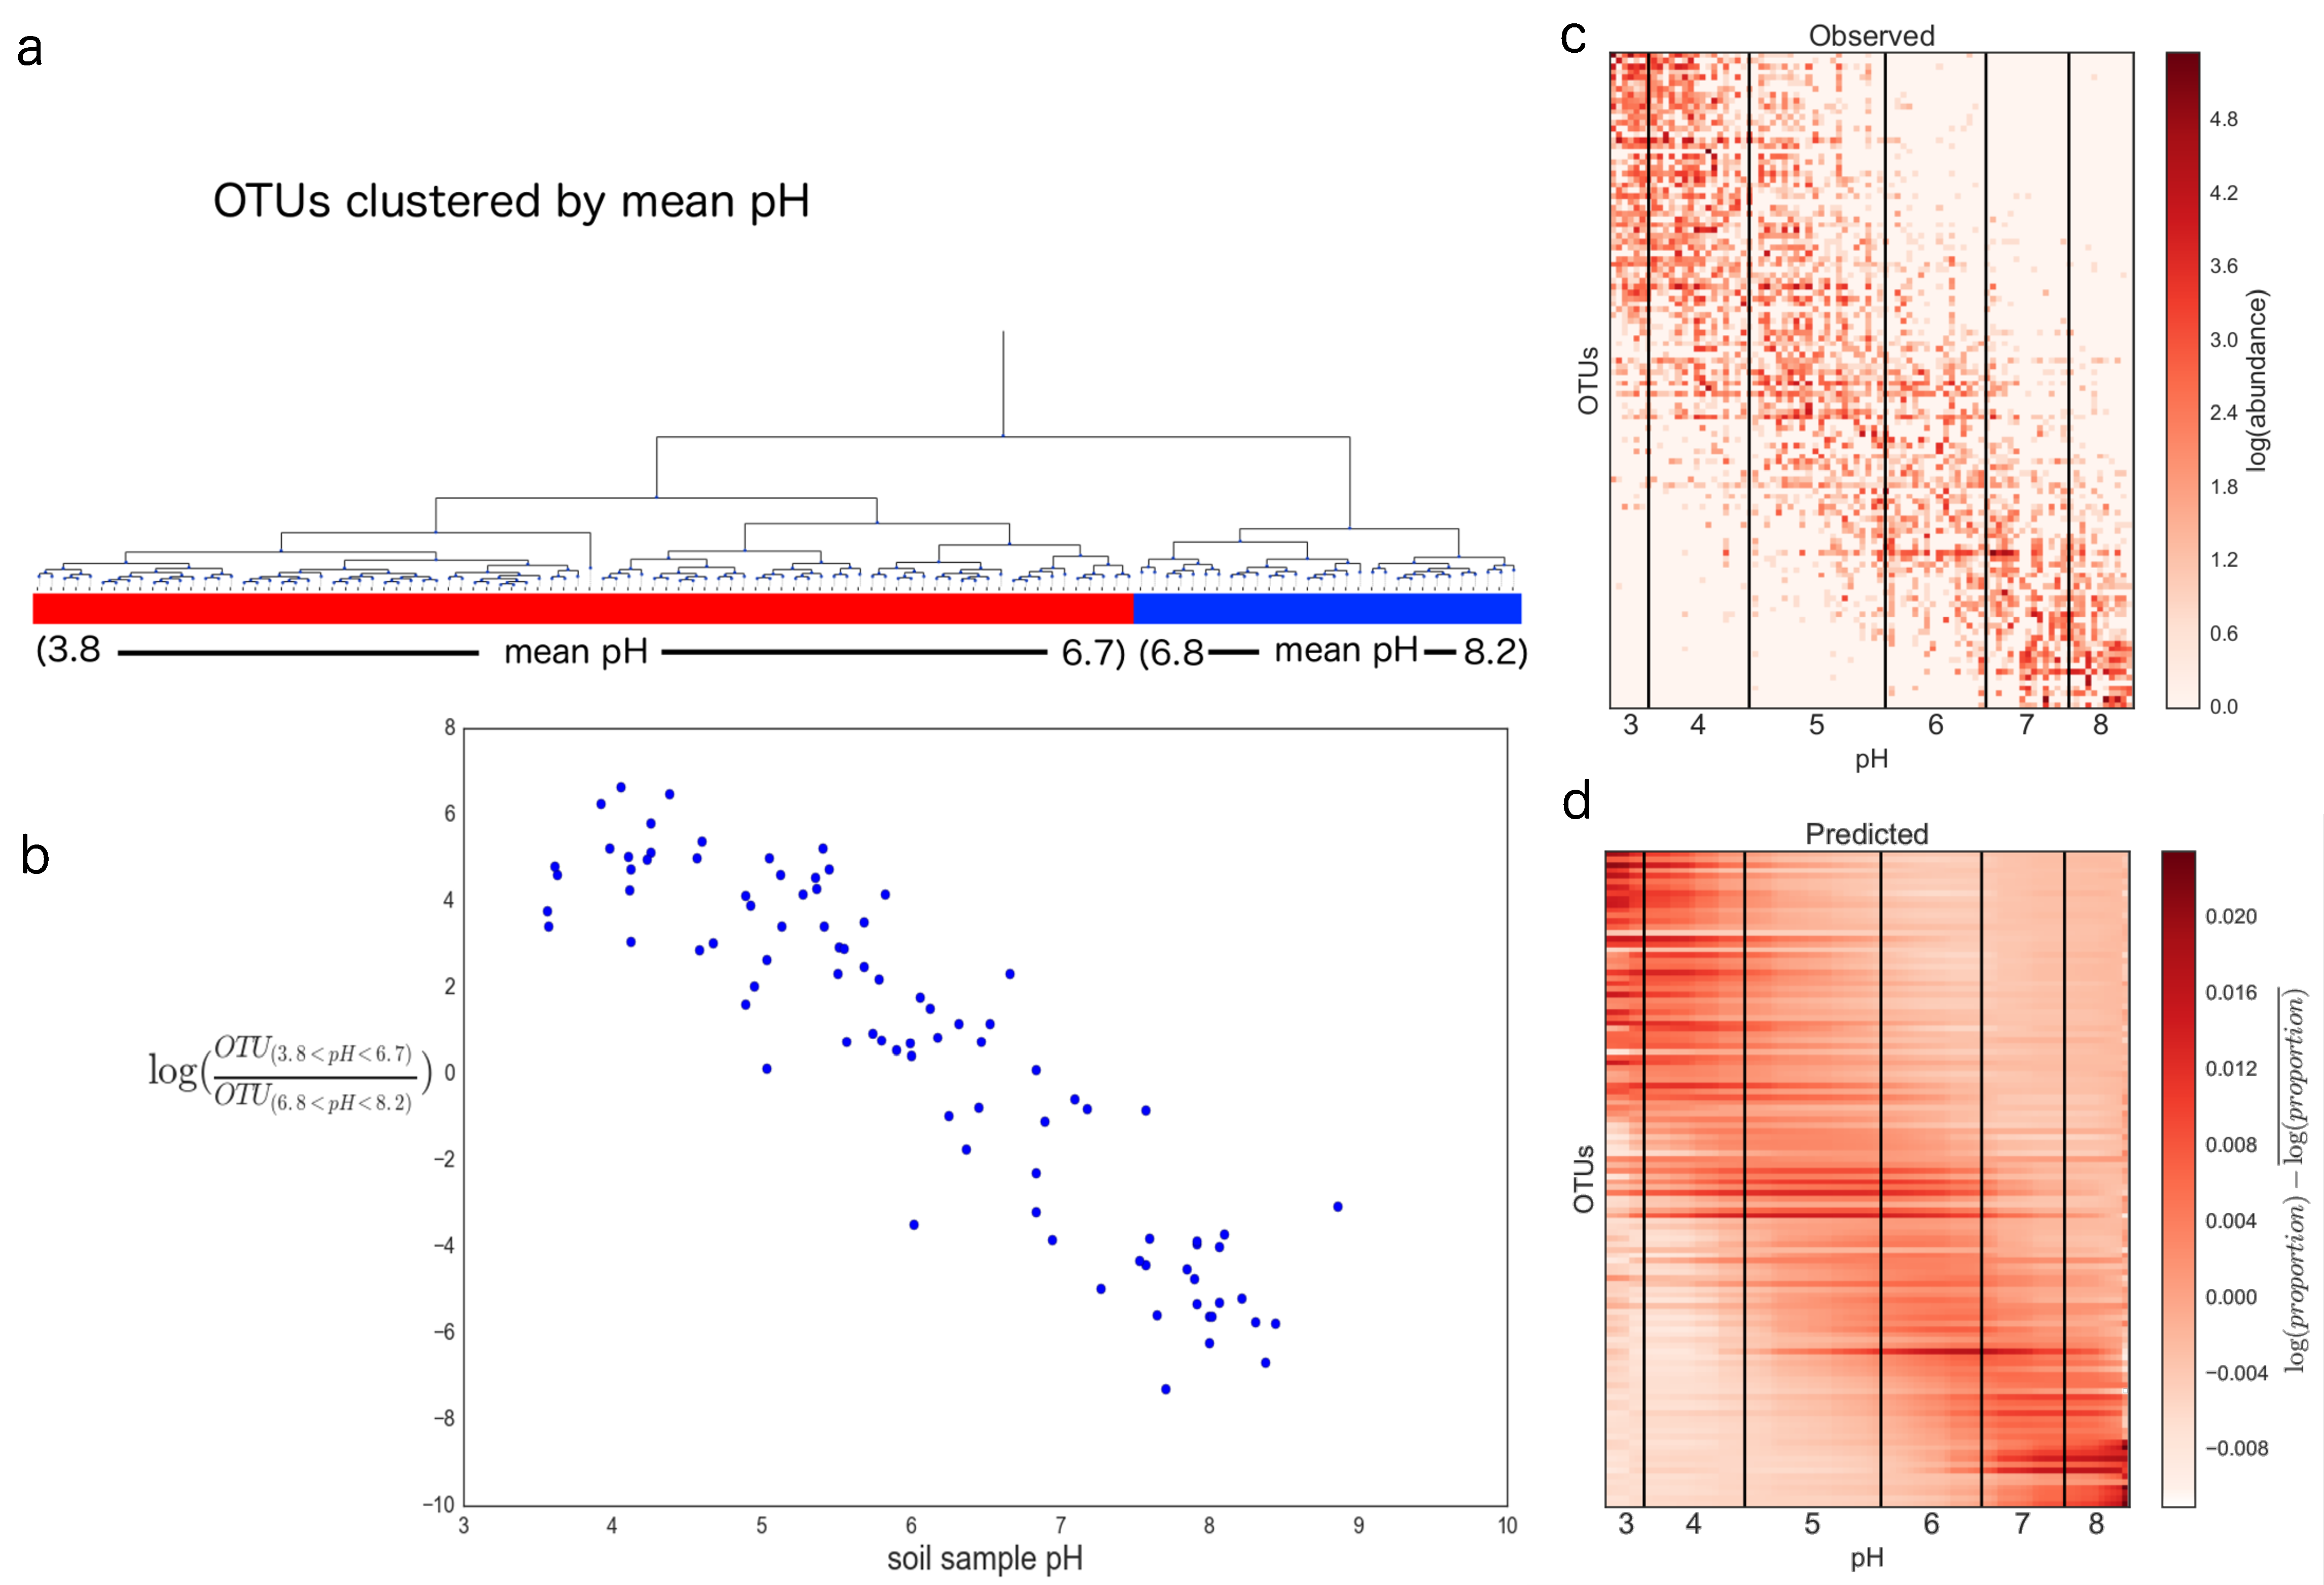
\includegraphics[width=1\textwidth]{ch3/Figure2.pdf}
        \caption[The application of balances on a soil microbial dataset to identify
          microbial partitioning with respect to pH.]
        {The application of balances on a soil microbial dataset to identify microbial partitioning with respect to pH.(a) Hierarchical clustering of closed ref \gls{otu}s based on mean pH. (b) The balance of low pH associated organisms (3.8 $<$ mean pH $<$ 6.7) and high pH associated organisms (6.8 $<$ mean pH $<$ 8.2). (c) Observed \gls{otu} counts sorted by pH. (d) Predicted \gls{otu} proportions from ordinary least squares linear regression on balances sorted by pH. The coefficient of determination was 35\%, showing that 35\% of the variation in the microbial community abundance data can be predicted by pH alone.\index{SanDiego8}}
        \label{figc2}
 \end{figure}
 At a first glance, uncovering the true correlations correct appears to be a hopeless cause.  This is where balances become useful.  Rather than attempting to correlate individual phyla against pH, we will group \gls{otu}s together according to their difference in mean pH (Figure \ref{figc2}a), and investigate how these balances of groups changes with respect to pH (See Materials and Methods on hierarchical clustering).  This circumvents the dependence issue noted previously.  We do not need to worry about subgroups within the left and right subtrees of a balance to be influencing each other, due to the independence property shown in Figure \ref{figc1}ef.  \par
 The balance concept proves to be a very powerful technique for investigating how these groups of organisms change relative to each other as pH increases.  Recall the cartoon example in Figure \ref{figc1}d.  If there are two distinct unimodal species distributions, the balance pivots from being weighted by Red in low pH, to being weighted by Blue in high pH.  The exact same phenomenon is occurring here, except there are multiple species on left end of the balance, and multiple species on the right end of the balance.\par
 As shown in Figure \ref{figc2}b, there is a well defined trend of low pH \gls{otu}s (3.8 $<$ mean pH $<$ 6.6) gradually being overtaken by high pH \gls{otu}s (6.7 $<$ mean pH $<$ 8.2) as the pH increases, forming a nice linear trend defined by the top balance in the tree shown in Figure \ref{figc2}a.  If we were to sort the samples by their mean pH, and the \gls{otu}s by their mean pH (Equation 3), a well defined band pattern appears.  Here, it is clear that \gls{otu}s with a mean pH less than 3 rarely have nonzero counts above 8.  Likewise, \gls{otu}s that have a mean pH more than 8 rarely have nonzero counts below 3.  If we were to tie in this band pattern in Figure \ref{figc2}c together with the balance vs pH trends shown in Figure \ref{figc2}b, we would obtain a very different interpretation from the original study.  \gls{otu}s tend to be observed in very specific pH ranges, but not commonly observed outside of these ranges.  This ties together with some concepts in niche theory - \gls{otu}s are more suited to live within a designated range of pHs.  And if they are placed outside of this pH range, they are outcompeted by other organisms who are more suited to live within the given pH range.  \par
 These patterns were completely missed when only looking at the phylum level in the original study.  In fact, based on the calculated mean pH values for each \gls{otu}s, it is observed that \gls{otu}s from all of the phyla mentioned in the study are widely distributed across the pH gradient (Supplemental Table 1).  As an extreme example, \gls{otu}s from the family Bradyrhizobiaceae were observed to be present in both ends of the spectrum, some present at pH values as low as 5.36, while others present at a pH as high as 6.75.  These are astronomical differences, considering
 that 95\% of the \gls{otu}s have a mean pH that falls between this range. This provides additional justification for building a tree based on mean pH, rather than bacterial phylogeny.\par
  Finally, these balances can be used to build predictive models.  Using ordinary least squares on the calculated balances, the entire microbial community profile can be predicted using pH alone with an $R^2$ of 0.35. This means that pH alone explains over 35\% of the total variation in entire soil microbial communities across North and South America. The resulting fit can be transformed back to proportions to yield the predicted proportions (Figure \ref{figc2}d).  From this heatmap, the key patterns are still retained, such as the band pattern apparent in Figure \ref{figc2}c. There are many regression techniques published that attempt to use microbial abundances to predict covariates, such as the post-mortem interval \cite{mammalian_corpse} or body mass index \cite{microbial_regression}. This approach is the first of its kind to attempt to address the reverse problem to predict entire microbial community distributions based on environmental variables. These predictions were enabled by the powerful fundamental properties of balances.\par
  \subsection{Case Study \#2 – Balances of pH-driven subcommunities in a lung sputum culture microcosm}
 In this study, lung sputum samples were collected from 16 cystic fibrosis (\gls{cf}) patients.  These sputum samples were then grown in a capillary tube culture system (Winogradsky Cystic Fibrosis system) that mimics the conditions of a lung bronchiole \cite{wincf}.  These samples were placed into separate tubes and the pH of the media was adjusted from 5 to 8.5 at intervals of 0.5 to determine how the microbial community changed with respect to pH.  After growth in the capillary tubes, the communities were assessed using 16S \gls{rrna} gene amplicon sequencing.\par
 One of the difficulties in this study was characterizing pathogenic bacteria.  Early on in this case study, the only significant finding discovered was that patients had different lung sputum microbiomes (Figure \ref{figc3}a). It was hypothesized that there was a subcommunity of low pH organisms and a subcommunity of high pH organisms that periodically appeared and disappeared in \gls{cf} lung sputum.  However, these changes could not be detected using available statistics, likely due to the compositionality problem.  Since the different \gls{cf} patients had idiosyncratic lung communities, they ended up having different \gls{otu}s responding across the laboratory pH gradient, yielding insufficient statistical power to detect changes in any given \gls{otu}.  As a result, when these lung sputum communities were placed into different media and studied, it was not clear exactly what organisms were a part of this low pH or high pH subcommunity.  \par
 Balances are a natural solution to this problem.  In addition to probing for similar patterns to those observed in the previous study, balances are well adapted as a transformation for standard statistical analyses.  Since Euclidean operations directly translate into perturbation and powering operations on proportions \cite{ilr, Pawlowsky-Glahn2015-qb}, many of the publicly available statistical tools can be applied to directly to balances.  For this study, we opted to use Linear Mixed Effects models to test for pH differences while simultaneously accounting for all of the differences between lung microbiomes across \gls{cf} patients.   Based on prior analyses with pH in soils, the tree was built using the exact same strategy (See Methods and Materials).   Significant balances testing for pH were determined with a p-value cutoff at 0.05 after Bonferroni correction.  \par
  \begin{figure}[H]
        \centering
        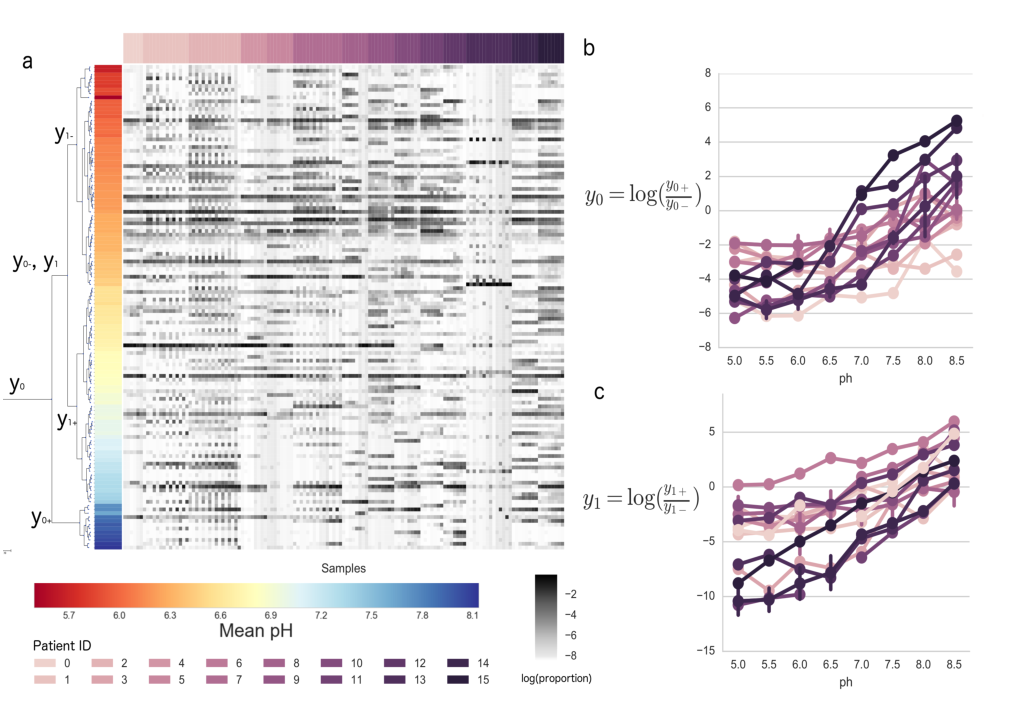
\includegraphics[width=1\textwidth]{ch3/Figure3.pdf}
        \caption[The application of balances on a cystic fibrosis dataset to identify
          microbial partitioning with respect to pH.]
        {The application of balances on a cystic fibrosis dataset to identify microbial partitioning with respect to pH.(a) A bifurcating tree generated from hierarchical clustering of \gls{otu}s based on mean pH.   The size of the internal nodes is inversely proportional to the p-value of the linear mixed effects model test on pH for that given balance.  A heatmap of all of the \gls{otu} abundances sorted by patient. \gls{otu}s were log transformed and centered across rows and columns. These abundances are aligned with the tips of the tree.  (c) The progression of the top balance over the pH for all of the patients.  (d) The progression of the second top balance over pH for all of the patients.\index{SanDiego8}}
        \label{figc3}
 \end{figure}
 A heatmap relating pH to \gls{otu} abundances across these samples does not yield clear trends (Fig 3a).  But even though we don't see a clear pattern in the heatmap, with the balance approach, we can still observe niche differentiation across the pH gradient.  In Figure \ref{figc3}b, y0 represents the log ratio of all of the high pH \gls{otu}s (7.6 $<$ mean pH $<$ 8.12) over all of the low pH \gls{otu}s (5.4 $<$ mean pH $<$ 7.4).  As the pH of the samples increases, the balance increases, likely because the low pH \gls{otu}s are becoming increasingly less abundant compared to the high pH \gls{otu}s (p-value=$7.5 \times 10^{-46}$).  The same pattern is even more apparent in y1 (Figure \ref{figc3}c). The low pH \gls{otu}s (5.4 $<$ mean pH $<$ 6.4) become increasingly less abundant than high pH \gls{otu}s (6.5 $<$ mean pH $<$ 7.4) as the sample pH increases (p-value=$2.25 x 10^{-67}$).  When Bonferroni multiple hypothesis correction was applied to these tests, the p-values were rounded down to zero.  While these patterns were not obvious when looking at the raw proportions, the balance tree approach shows very well defined trends among groups of \gls{otu}s. This can be done because even though individual \gls{otu}s may be sporadically distributed across the original samples, \gls{otu}s that thrive in similar pH niches grouped together on the environmental balance tree.  It is clear from Figure \ref{figc3}b and c that there is a transition from low pH organisms to high pH organisms along the pH gradient.  Even though the \gls{cf} patients don't have the same lung microbiomes, they contain \gls{otu}s that behave the same with respect to pH.  This pattern would not have been nearly as apparent without clustering the \gls{otu}s by mean pH and accounting for the patient effects in the linear mixed models.
 \section{ Discussion}
 In this study, we have demonstrated the benefits of applying balances to infer niche differentiation in microbes.  In the first case study, we have outlined the challenge of performing correlations of \gls{otu}s versus environmental variables, and showed how balances can capture information about species turnover across the pH gradient, which allowed us to build a model to predict microbial proportions based on pH alone.  In the second case study, we identified the challenges of studying individual \gls{otu}s due to similar niches being occupied by drastically different \gls{otu}s across different patients. Balances coupled with linear mixed models allowed us to obtain more statistically robust results, which were also more informative with respect to the differences in distribution of microbes across environmental niches.\par
 There are numerous additional benefits of analyzing species balances instead of individual species counts.  First, balances are known to be scale-invariant, so balance trees naturally correct for differences in sequencing depth without requiring rarefaction (Equation S1) and avoid many of the limitations associated with this procedure \cite{waste_not}. Second, balances are sub-compositionally coherent, which means that changes in non-overlapping sub-communities do not impact each other.  For instance, in Figures 1e and 1f, the Purple population triples, and balances, and change because they explicitly contain the Purple species.  In contrast, does not change between these two scenarios because it does not relate to the Purple species (in fact, it only accounts for the Red and Green species).  This is not the case when observing the raw proportions, from which it appears as though everything is changing, even though the Purple species is the only changing species.  This phenomenon has previously been noted \cite{ancom} and can lead to extremely high false positive rates with some standard statistical techniques such as Pearson correlations or t-tests on proportions.  More discussion about this issue can be found in Figure S1. Third, arithmetic operations on balances directly translate into perturbation and powering operations on proportions \cite{ilr, Pawlowsky-Glahn2015-qb}, which can capture information about relative growth and decay of species.  This ultimately opens the door for applying standard statistical techniques, such as multiple linear regression \cite{c24} and linear mixed effects models nested design statistics directly to balances, providing additional justification for the analyses performed in the case studies.  We have shown this in the two case studies.  Finally, balances are permutation invariant.  Species can be sorted in any order deemed appropriate.  Along the same lines, these species can be rearranged into any arbitrary grouping represented as a bifurcating tree.  These trees can be built to address the questions at hand, whether it be studying species turnover across pH gradients, or even uncovering the relationships between phylogenetic clades.  In fact, balances can be thought of as be utilized as an ordination technique, since every bifurcating tree forms an orthonormal basis in the Aitchison Simplex \cite{groups_of_parts}.\par
 Although the concept of balances does not address questions about properties of individual bacteria, it does answer higher-level questions concerning interactions among groups of organisms, which are arguably much more interesting from an ecological point of view. These questions can be based either on the phylogenetic tree of the bacterial community, or on environmental clustering.  There is still room for improvement on utilizing balances.  For example, the issue of zeroes still remains, because the logarithm of zero is undefined.  Currently, the common approach is to add a pseudo-count \cite{dealing_with_zeros}.  However, an appropriate tree choice can mitigate this issue, because the zeroes can be explicitly aggregated in some scenarios (Figure S2 and Figure S3).  Along the same lines, issues can arise from low-coverage samples.  If sampling is not saturated, many \gls{otu}s have low read counts, and the balances towards the tips of the trees can be highly volatile.  This is because the absolute change between one or two reads may be small for low abundance \gls{otu}s, but this will lead to large changes in log ratios, which lead to spurious signals at the tips of the tree.  As a rule of thumb, balances towards the root of the tree are more trustworthy than those at the tips of the tree.\par
 The balances approach will be key for analyzing functional roles of \gls{otu}s.  It is known that in environments like the human gut, people share very few \gls{otu}s with each other, but have roughly the same proportions of functional genes \cite{soil_pyro}.  This suggests that there is substantial functional redundancy across \gls{otu}s, which has been observed previously in time series studies in the context of infection \cite{microbiome_timeseries} — in other words, in these microbial communities many players might be sporadically distributed across similar niches.  This phenomenon could explain the sparse nature of 16S relative abundance data, and why similar environments such as human guts share few common \gls{otu}s.  Such distributions pose tremendous challenge to analyses based around identifying the niche occupancy of individual \gls{otu}s. By instead permitting the statistical comparisons to be performed across nested groups of \gls{otu}s with similar distributions, it becomes possible to robustly identify patterns of niche differentiation without requiring sufficient information be present in the abundances of each individual taxon. Identifying common functional roles of potentially diverse organisms, and analyzing the balances between these groups could significantly simplify analyses in future amplicon studies.  The ability to construct such trees would enable rapid characterizations of environmental niches, and the corresponding functional roles of the microbes occupying in these niches.\par
 All in all, balance trees are an extremely powerful tool for analyzing relative abundances and uncovering patterns associated with niche differentiation, while avoiding the issues associated with compositionality and enabling the application of conventional statistical tools.  This will ultimately open the doors for extensive mining of ecologically relevant patterns.
 \section{Methods and Materials}
 All analyses can be found in the attached IPython notebooks.  The core functions required to perform the balance basis calculations, tree visualization tools, and statistical analyses can be found in \url{https://github.com/biocore/gneiss}.  The IPython notebooks used to carry out all of the analyses can be found in the gneiss repository.  All code has been extensively unit-tested and documented. \par
 The core compositional statistics and tree data structures were are part of scikit-bio 0.4.1 and beyond. The hierarchical clustering was performed using Scipy.  Pandas and \gls{biom} \cite{biom} were used to store and manipulate the \gls{otu} tables and the metadata files.  Seaborn, matplotlib and ETE \cite{ete} were used for the visualizations.\par
 The isometric log ratio transform is an isomorphism (i.e. a function) that can map proportions to balances one to one \cite{ilr}.  These balances can be calculated as shown in Equation 1. Alternatively, they can be calculated using a linear transformation with an orthonormal basis e. This orthonormal basis can be calculated as follows
 \begin{equation}
        e_{l}=C\left [\exp(\: \: \underset{k}{\underbrace{0,...0}},\underset{r}{\underbrace{a,...a}},\underset{s}{\underbrace{b,...b}}, \underset{t}{\underbrace{0,...0}}) \right]
 \end{equation}
 \begin{equation}
        a=\frac{\sqrt{s}}{\sqrt{r(r+s)}} \quad  and \quad b=\frac{-\sqrt{r}}{\sqrt{s(r+s)}}\notag
 \end{equation}
 where $e_{l}$ refers to the balance axis aligned with the internal node \textit{l}. $C[x]$ denotes the normalization operation to normalize all of the \gls{otu} abundances to proportions that add up to 1.  $r$ refers to the number of tips in the left subtree, $s$ refers to the number of tips in the right subtree, $k$ refers to number of tips to the left of the left subtree and $t$ refers to the number of tips to the right of the right subtree. Since $e$ forms an orthonormal basis, it must have unit norm and every pair of axes in $e$ must be orthogonal.  The square root term   in Equation 1 is a normalization factor which was required for unit norm in Equation 2 (12).    Since it is not possible to take a logarithm of zero, a pseudocount of 1 was added to all of the abundance.  While this is a problem being addressed by the field, this technique is one of the more commonly used techniques \cite{dealing_with_zeros}.\par
 The mean pH used for the 2 case studies was calculated as follows.
 \begin{equation}
        \overline{g}_{x}=\sum_{i=1}^{N}g_{i}\frac{x_{i}}{\sum_{j=1}^{D}x_{j}}
 \end{equation}
 Where $x_{i}$ is the proportion of \gls{otu} \textit{x} in sample \textit{i} , $g_{x}$ is the mean pH of \gls{otu} \textit{x}, and $g_{i}$ is the sample pH at sample \textit{i}. This calculation can be found in the gneiss package under the function \textbf{mean\_niche\_estimator}. The function used to sort the tables in Figure \ref{figc2}c used \textbf{niche\_sort}. The resulting tree was built using UPGMA \cite{upgma} is shown in Figure \ref{figc2}a and Figure \ref{figc3}a, and can be generated using the scipy linkage function.\par
 This regression model is implemented in gneiss under the \textbf{ols} function.  The analysis can be found in the IPython notebooks on the gneiss repository under the ipynb folder in \textbf{88soils.ipynb}. To focus on the highest abundant organisms, only \gls{otu}s that had more than 100 reads in the entire study were considered.\par
 The linear mixed effects model is implemented in gneiss under the \textbf{mixed} functions, and the analyses can also be found in the IPython notebooks in the ipynb folder in \textbf{cfstudy.ipynb} In case study 2, only \gls{otu}s that had more than 500 reads were considered.   \par
 The Win\gls{cf} system was used according to the methods in \cite{wincf}, except only the pH dye media variable was used. The media was buffered at 0.5 units of pH from 5 to 8.5 using calculated proportions of phosphate buffer and NaOH or HCl. Sputum samples were collected from \gls{cf} patients after expectoration or induced expectoration of sputum according to the UCSD IRB approved project \#081500, and were inoculated in triplicate into capillary tubes containing the eight different pH buffered media. These eight sets of tubes in triplicate from 18 patients was then incubated at $37^{o}$C for 48 hours. The media was then removed, bacterial DNA extracted, and variable region 4 of the 16S \gls{rrna} gene was amplified and sequenced on the Illumina MiSeq platform using Earth Microbiome Project benchmarked protocols \cite{illumina_microbes, global_patterns}.  Data were processed using QIITA and \gls{otu}s were calculated using closed reference clustering at the 97\% identity cutoff for both the 88 soils and the \gls{cf} study.
\section{ Data availability}
Data for case study 1 was retrieved from Qiita (study ID 103). Data from case study 2 was retrieved from Qiita (study ID 10511).
\section{Acknowledgements}
We first acknowledge Jonathan Friedman for the original idea of applying balances to analyze microbial communities. We also acknowledge Justin Silverman and Lawrence David, in addition to Liam Toran, Tomasz Kosciolek, and Amnon Amir, for their insights and discussion on balances. In addition, we are grateful for the input from Christian Lauber and Noah Fierer concerning case study 1. Finally, we thank all of the scikit-bio developers, especially Jorge Cañardo Alastuey, Evan Bolyen, Jai Rideout, and Greg Caporaso, for reviewing the compositional statistics submodule in scikit-bio.

J.T.M. was funded by NSF grant GRFP DGE-1144086 and NSF grant IGERT 1144807 under the IQ Biology program at the University of Colorado Boulder. R.A.Q. was funded under the Cystic Fibrosis Research Innovation Award from Vertex Pharmaceuticals. This work was funded under Alfred P. Sloan Foundation grants G-2015-13933 and G-2015-13979 and National Institute of Diabetes and Digestive and Kidney Diseases (NIDDK) grant P01DK078669.

J.T.M. led the software development, benchmarking, and manuscript writing and developed the idea of applying regression to balances. J.S. contributed the idea of applying linear mixed-effects models to balances and named the software package. R.A.Q. collected the \gls{cf} lung sputum samples. D.M., A.G., J.A.N.-M., and Y.V.-B. reviewed the code in Gneiss. M.L. reviewed the mathematical notation. All authors wrote and proofread the manuscript.

Chapter 3, in full, is a reprint of the material as it appears in
``Balance Trees Reveal Microbial Niche Differentiation''
James T. Morton, Jon Sanders, Robert A. Quinn, Daniel McDonald, Antonio Gonzalez,
Yoshiki Vázquez-Baeza, Jose A. Navas-Molina, Se Jin Song, Jessica L. Metcalf,
Embriette R. Hyde, Manuel Lladser, Pieter C. Dorrestein, Rob Knight
\emph{mSystems}, 2, 2017.  The dissertation author was the primary investigator and first author of this paper.


\chapter{Establishing microbial measurement standards with reference frames}
Approaches to differential abundance analysis have been controversial across the microbiome sciences.
The current gold standard requires laborious measurements of total biomass to accurately determine shifts
in microbial abundance among samples. Here, we highlight the pitfalls of comparing relative abundance across
samples and identify two solutions that reveal microbial changes without the need to estimate total biomass.
In an oral time series experiment, these methods alleviate false positives and produce consistent results
on both raw and cell count normalized data. Further, these methods identify differentially abundant
microbes previously undetectable with standard methods in two independent published atopic dermatitis
datasets. These methods therefore allow re-assessment of published relative abundance data to reveal
previously undetectable microbiome changes without the need for new molecular assays.
\section*{Introduction}
Next-generation microbiome sequencing provides data in the form of relative abundances,
independent of the total biomass of the original sample. Numerous analytical approaches
including rarefaction \cite{Weiss2015-gn}, median \cite{Love2014-sn}, and quantile normalization
\cite{Paulson2013-mm} have been proposed to make biological samples more comparable to each other.
However, these analytical solutions do not control for false discovery rates \cite{Russel2018-na},
\cite{Hawinkel2017-ax} and could even be a source of reproducibility issues observed in microbiome
studies \cite{Gloor2015-zq}. Here, we overcome these mathematical challenges in analyzing
compositional data in the context of microbiome sequencing data by presenting and utilizing
the notion of “reference frames” for inferring changes in abundance. We confirm our ability
to make the same inferences as one makes with absolute abundances by quantifying microbial load
in unstimulated saliva before and after brushing teeth, and analyzing 16S \gls{rrna} gene amplicon sequencing
data.  Finally, we analyze one published and one new skin metagenomic dataset and show that by analyzing
the ratios of taxa, or using a novel method of ranking taxa by their differential abundance as ratios of
proportions, we can find stable reference frames of compositional change and overcome the challenges
inherent in comparing relative abundances.\\[5 mm]
%
To illustrate pitfalls of comparing relative abundance data, consider the following toy example
in Figure 1. Here we have two samples collected  before and after a given treatment.  In the
scenario in Figure 1a, there are only two different taxa, colored orange and blue, that are in
equal proportions. The true sample is everything inside the large oval, but by sequencing we are
only observing a fraction of this sample, represented here by the taxa in the concentric dashed
oval labelled ‘observed’.  In the after treatment, we show two possible scenarios. Both observe
the same 2:1 ratio of orange to blue, and it is tempting to conclude from the relative abundances
that orange increased and blue decreased.  However, the true samples could differ dramatically
in their total microbial load. In the bottom scenario in Figure 1a, both orange and blue taxa
increase compared to the before sample, but the orange taxa increase more. Alternatively, in the
top scenario the number of orange taxa remains constant, and the number of blue taxa decrease.
Because we only observe an equal number of sequences, however, we cannot differentiate between
these two biologically important outcomes. In fact, there could be an infinite number of outcomes
that provide the same 2:1 ratio of orange to blue. This greatly complicates the generation of a
meaningful null hypothesis, and can cause misleading p-values if this phenomenon is not taken
into consideration.\\[5 mm]
\begin{figure}
  %%%\includegraphics{something} % this command will be ignored
  \centering
  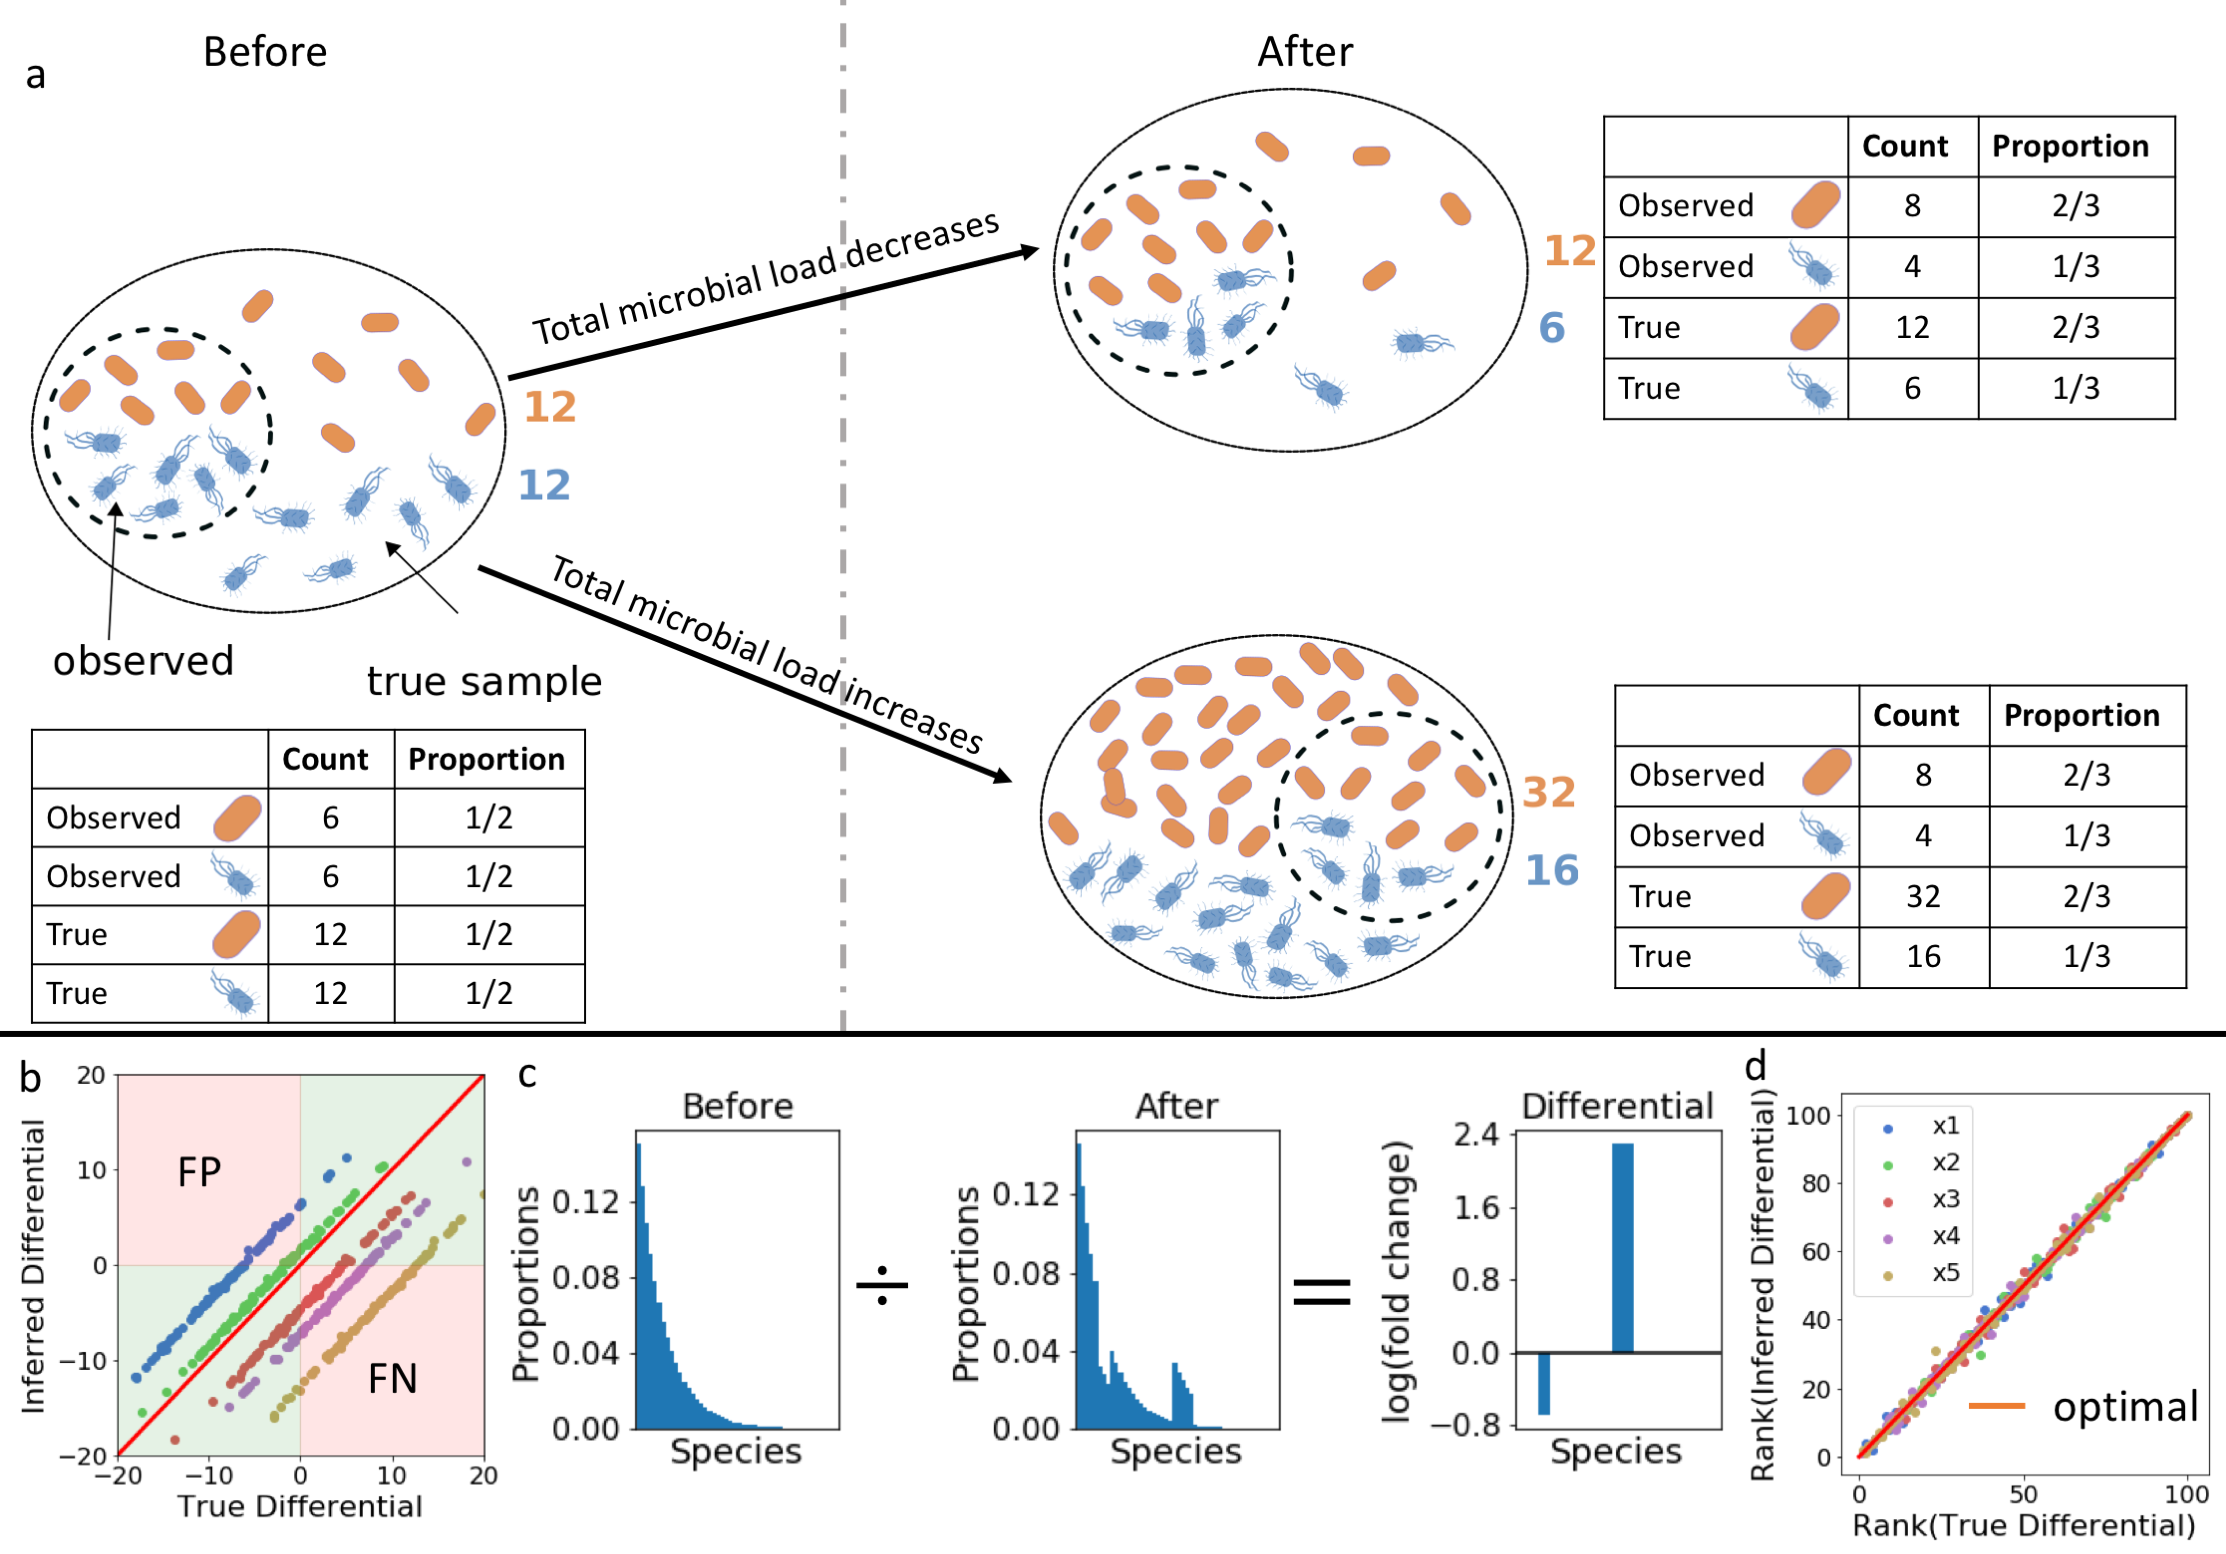
\includegraphics[width=1\textwidth]{ch4/Figure1.png}
  \caption[Illustration of total population size bias and the concept of differentials.]{
    Illustration demonstrating statistical limitations inherent to compositional datasets. (a) On the left,
    we have a scenario before a hypothetical treatment. On the right, we have a scenario after a hypothetical treatment.
    Two different scenarios can yield the exact same proportions in the after treatment. (b) Simulated datasets
    plotting the true differential from absolute data on the x-axis, versus the inferred differential from relative
    data on the y-axis. Each dot represents a taxa in the dataset, and the colors represent datasets with various
    ratios of total microbial load between before and after samples. The red line represents the optimal scenario
    where the samples have equal microbial load. This illustrates the prevalence of either false positives (\gls{fp}) or
    false negatives (\gls{fn}) when performing differential abundance analysis on samples with unequal total microbial load.
    The presence of either \gls{fp}s or \gls{fn}s is dictated by a nonlinear function of the true differential (see online methods).
    (c) An illustration of differential proportions of bacterial species before and after treatment. (d) Same data as
    (b) but plotting the rank of the differentials, demonstrating that ranks are equivalent independent of differences
    in microbial load.}
\end{figure}
%
%
Microbiome measurements from next-generation sequencing are inherently compositional. Samples are
typically collected from a much larger environment (e.g. fecal material from the gut, or water
sample from the ocean).  From these samples, a subset is separated for DNA extraction (e.g. swabbing
a fecal sample, or aliquoting a water sample). A subset of this DNA is then used as input for the PCR
reaction, and a subset of amplicon is pooled into a library, and a subset of the library is sequenced.
By the time that quality-filtered sequencing data is obtained, this data reflects only a small subset
of the true environment, and is not an accurate reflection of microbial load in the original sample
\cite{Vandeputte2017-jl}. Without knowledge of the total microbial load in the environment, we cannot
differentiate between the infinite number of possible scenarios governing which microbes increase and
decrease in abundance. This phenomenon has been shown to lead to close to 100\% false positive rates
in conventional statistical tools \cite{Mandal2015-xw,Morton2017-dz}.  \\[5 mm]
%
In order to properly infer true differences between individual microbes, one must measure the size of
the total population. This means that computing the change between samples using relative abundances
will introduce bias resulting from the lack of information concerning the total microbial load (online
methods Equation 2). Simulated data in Figure 1c shows how different biases (i.e. ratios between total
microbial loads) can cause either false positives or false negatives. \\[5 mm]
%
Multiple approaches at each level of sample processing have been proposed to quantify total microbial
load from environmental samples. At the sequencing level, adding a known amount of reference DNA not
expected to be present in the samples of interest has been used to extrapolate the amount of starting
material \cite{Smets2015-od, Tkacz2018-fp}.  Normalization by this method is complicated due to
calibration challenges of choosing the proper amount of internal standard \cite{Tkacz2018-fp,Smets2015-od}.
At the extraction level, quantitative PCR (\gls{qpcr}) of genomic DNA with ‘universal’ primers against the 16S
\gls{rrna} gene can be used to estimate total microbial load \cite{Nadkarni2002-og}. However, it is impossible
to escape primer bias because no perfect primer pair can equally amplify all \gls{rrna} genes across species.
Furthermore, both spike-in and \gls{qpcr} include the issue of various subsetting as discussed above. Finally,
quantifying microbial load with flow cytometry allows for evaluation of primary sample, and is agnostic
to nucleotide sequence. A recent study has shown that adding quantitative information from flow cytometry
to microbiome analyses can dramatically improve interpretation of 16S amplicon sequencing data
\cite{Vandeputte2017-jl}. However, this technique requires expensive equipment and experienced users,
and tends to be low throughput. \\[5 mm]
%
The absolute abundance of a community, however, is only one dimension of measurement among the hundreds
to thousands of dimensions measured in microbial relative abundances; if you know the abundance of a
single species, and the relative abundance of all species, you can compute the absolute abundance of
all species. As such, a lot of information rests in relative abundances and important insights can be
gleaned without costly absolute abundances. We show that through existing methods and a novel,
conceptually integrative method, one can make stable inferences of abundance changes without requiring
a costly and throughput-limiting single dimension measurement. We verify with mathematical proof and
empirical data that our inferences are equivalent to those obtained from data containing absolute abundances.\\[5 mm]
%
Analyzing compositional data requires choosing reference frames for inferring changes in abundance.
By “reference frames” , we draw on the concept from physics by which one measures velocity “relative to”
another moving object. The concepts are related, and provide a useful means of understanding how to make
stable inferences with compositional data. As microbial populations change, we can contain our inferences
to how microbial populations change relative to reference frames given by other microbial populations.\\[5 mm]
%
Compositional data are commonly analyzed using log-ratios, and the choice of numerator and denominator
in a log-ratio determines our reference frame for inferring changes. The “centered log-ratio” uses the
mean of all sequences as a reference frame, measuring changes of one species' abundance relative to the
mean of all species, analogous to astrophysicists measuring the movement of Earth relative to the center
of mass in the Milky Way. Log-odds analyses use “all other sequences” as a reference frame, measuring the
change of one species relative to the rest. Several recently developed tools for analyzing sequence count
data differ in the reference frames used for making inferences. Ph\gls{ilr} \cite{Silverman2016-he} uses sister
clades as reference frames for one-another. Phylofactorization\cite{Washburne2017-up} iteratively
partitions reference frames of species separated by edges in the phylogeny. Morton et al.
\cite{Morton2017-dz} found reference frames through hierarchical clustering.\\[5 mm]
%
Here, we empirically validate the stability of compositional tools for sequence count data analysis and
propose a rank-based method for illustrating the distribution of possible reference frames and discovering
useful pairwise references for making reliable inferences of abundance change in compositional sequence-count
data. By ranking the log-ratio abundance changes (what we refer to as the “differentials”), one obtains an
accurate image of compositional change in a dataset and one can visualize candidate reference frames for
inferring changes (Figure 1c). As shown in Figure 1d, ranking the differential is independent of the
changes in the absolute microbial load, yielding an identical ranking of microbial differences between the
relative and absolute abundances.\\[5 mm]
%
Differentials can be estimated directly from using explicit count-based regression models. For example,
multiple works \cite{Silverman2018-ql,Aijo2018-jp, Grantham2017-gv,Xia2013-nd} have shown that multinomial
generalized linear models can infer differentials without adding pseudocounts to handle sampling zeros.
When estimating differentials, one can't determine whether a particular species went up or down in absolute
abundance, but only whether one species' change is higher or lower than others. These differentials can be
interpreted as feature importances or rankings commonly employed by machine learning methods.\\[5 mm]
\section{Results}
\subsection{Absolute quantification of unstimulated saliva microbes}
%
We demonstrate the utility of employing such tools in a 16S \gls{rrna} gene amplicon dataset of saliva samples
under a familiar scenario (tooth brushing) with matching quantitative flow cytometry data for validation.
Unstimulated saliva samples were collected from 8 individuals before and after brushing their teeth
(morning and night, n=32), and processed in parallel for microbial load quantification with flow cytometry
and 16S \gls{rrna} gene amplicon sequencing. Importantly, participants were asked to provide unstimulated saliva
for exactly 5 minutes, so in addition to estimating microbial concentration, we could obtain a proxy for
total microbial load in 5 minutes by taking into account salivary flow rate. As expected, total microbial
load significantly decreased after brushing teeth (Fig. 2a). By using analytical tools appropriate to
compositional datasets, we get the same results for differential abundance whether or not we normalize
our sequencing data to account for the change in microbial load. \\[5 mm]
\begin{figure}
  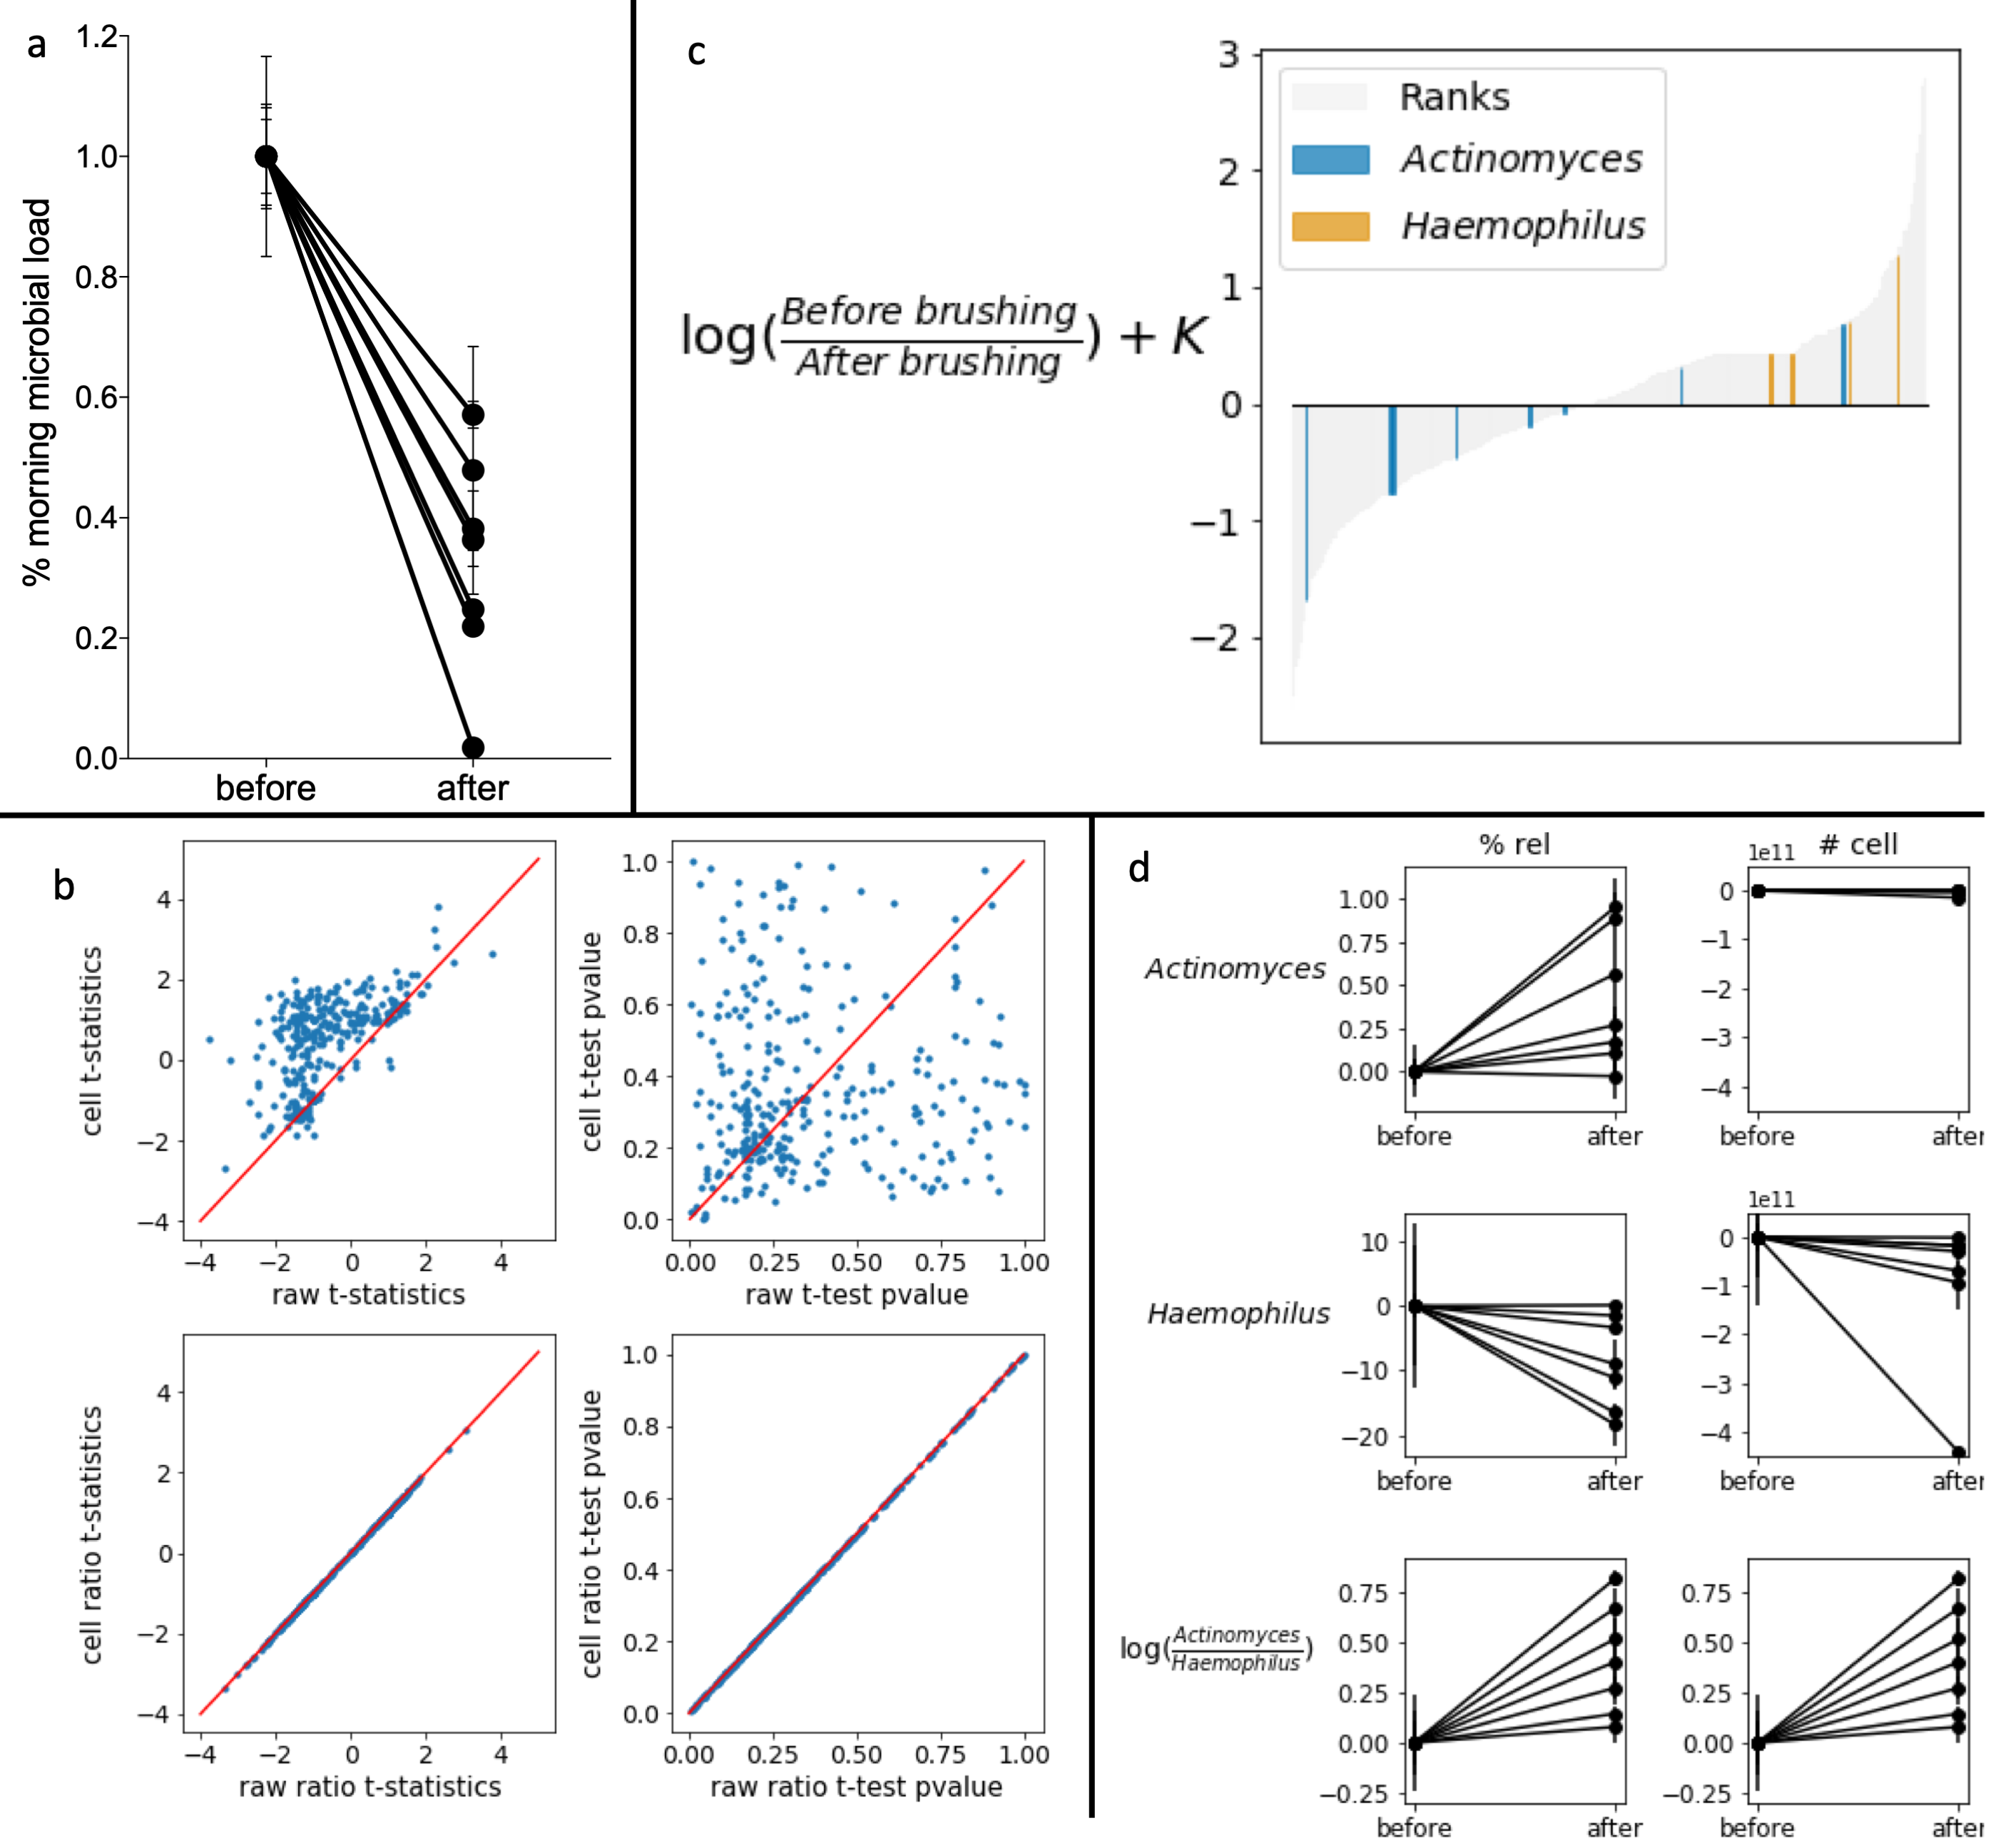
\includegraphics[width=1\textwidth]{ch4/Figure2.png}
  \caption[Comparison of absolute and relative abundance data using proportions, ratios and ranks on
    oral microbial communities.]{
    Analysis of salivary microbiota before and after brushing teeth. (a) Flow cytometry-quantified microbial
    load in unstimulated saliva collected for 5 minutes normalized to before brushing teeth. Each line corresponds
    to a different volunteer. (b) A comparison of t-statistics (left) and p-values (right) on individual taxa (top)
    and ratio between each taxa to \textit{Actinomyces} (bottom) between relative abundance data (x-axis) and cell
    count-normalized data (y-axis). (c) Microbial ranks estimated from multinomial regression applied to oral time
    series dataset with \textit{Actinomyces} and \textit{Haemophilus} highlighted.  The y-axis represents the log-fold change that is
    known up to some bias constant K, and the x-axis numerically orders the ranks of each taxa in the analysis
    (d) A comparison of relative abundance vs cell counts of \textit{Actinomyces}, \textit{Haemophilus} and log(\textit{Actinomyces}:\textit{Haemophilus})
    before and after brushing teeth. Only the differences since the before time point are visualized.}
\end{figure}
%
For both relative abundances and estimated cell counts, we performed paired t-tests to evaluate the change
in abundance of each taxon before and after brushing (Fig. 2b). It is clear that there are numerous false
positives resulting from applying t-tests to relative abundance data, given the disagreements between the
cell normalized and raw t-statistics (Spearman r=$0.53$) and p-values (Spearman r=$0.09$).  On the other
hand, if we instead focus on the ratio between \textit{Actinomyces} and the remaining taxa, the t-statistics and
p-values between the cell normalized and raw data are identical (Spearman r=$1.0$). Consequently, the
ratios are unaffected by microbial load, whereas the raw relative abundance values are affected as to
prevent meaningful inference.
%
From the differentials obtained from the multinomial regression (Fig. 2c), we can identify which taxa are
changing the most (highest and lowest log fold change - Table S1). Here, we highlight \textit{Actinomyces} and
\textit{Haemophilus}, which are on opposite ends of the spectrum. This suggests that \textit{Haemophilus} taxa are more prevalent
before brushing, and \textit{Actinomyces} taxa are more prevalent after brushing. When inspecting t-test results on
individual taxa in the relative abundance data, it appears that \textit{Actinomyces} significantly increased
(t-statistic=$2.89$, p-value=$0.013$) after brushing teeth and that \textit{Haemophilus} significantly decreased
(t-statistic=$-2.593$, p-value=$0.023$). But if we look at the cell counts, only \textit{Haemophilus} significantly
decreased (t-statistic=$-2.477$, p-value=$0.029$) (Fig. 2d). This is expected, because \textit{Haemophilus} is
typically found on the periphery of oral biofilms and was likely washed away during the brushing process,
whereas \textit{Actinomyces} is generally found on the surface of the tooth and acts as an anchor for biofilm
attachment \cite{Welch2016-lw}. \\[5 mm]
%
The log ratio of \textit{Actinomyces} and \textit{Haemophilus} between the relative abundances and the cell counts is identical.
While we cannot observe the decrease of \textit{Haemophilus} or the stability of \textit{Actinomyces}, with the log ratio of their
relative abundance, we can observe the interaction between these two taxa and the increase of \textit{Actinomyces}
relative to \textit{Haemophilus} after brushing teeth (t-statistic=$2.833$, p-value=$0.015$) without having the added
information from absolute abundances. Similarly, the log ratios of each species compared to \textit{Actinomyces} is
consistent between the relative abundance data and the cell normalized data (Fig. 2b, bottom plots).\\[5 mm]
%
This consistency between inferences made based off the relative and absolute abundances is crucial, because
in many circumstances it is not possible or practical to estimate total microbial load. For example, skin swabs
are often difficult to use in flow cytometry due to very low biomass and difficulty in transferring intact cells
from the swab into a liquid solution. Furthermore, skin samples are notoriously sensitive to 16S \gls{rrna} gene primer
choice making \gls{qpcr} quantification challenging. Similarly, for historically collected samples that now exist only
as DNA in a freezer or as sequences in a database, flow cytometry approaches are not feasible. \\[5 mm]
%
\subsection{Discovery of interkingdom relationships in atopic dermatitis}
%\\[5 mm]
The tooth brushing example provides ground truth for the method, but many clinically relevant microbiome questions
involve less obvious differences. We demonstrate how viewing relative abundances alone produces false negatives in
the context of an important skin disease, atopic dermatitis (\gls{ad}). \gls{ad} has a complex etiology, and many microbiome
studies performed using next-generation sequencing have focused on bacterial changes associated with \gls{ad}, with major
focus on the pathogen \textit{Staphylococcus aureus}. The yeast genus \textit{Malassezia} has also been implicated, although conflicting
results have been published as to which \textit{Malassezia} species are involved and whether they are more or less prevalent
in \gls{ad} \cite{Glatz2015-ag}. A recent shotgun metagenomic study examined the skin microbiome over time during an \gls{ad}
flare and recovery. They observed a decrease in \textit{Staphylococcus aureus} relative abundance in the healthy, recovered
skin (non-lesioned) compared to \gls{ad} flare (lesion), but no significant changes in the relative abundance of
\textit{Malassezia} species over time in these \gls{ad} patients \cite{Byrd2017-eb}.
%
However, applying compositionally coherent methods to this dataset revealed part of the story which was missing.
Observing the ranks from multinomial regression (Fig. 3a, TableS2), it is apparent that compared to lesioned skin,
\textit{S. aureus} is one of the taxa to decrease the most relative to all of the microbial species in the non-lesioned sites,
followed by \textit{S. epidermidis}, and \textit{M. globosa}. Consistent with the analysis of proportions
in (Fig. 3b) the ratio of \textit{S. aureus} : \textit{P. acnes} was significantly increased in flare
(t-statistic=$2.973$, p-value=$7.811 \times 10^{-3}$) and correlated with \gls{scorad} score, a clinical assessment
of \gls{ad} severity (Pearson=0.747, p-value=$3.516 \times 10^{-6}$). Contrary to previous findings, both
\textit{S. epidermidis} : \textit{P. acnes} and \textit{M. globosa} : \textit{P. acnes} were also significantly
increased in lesioned skin (t-statistic=$3.197$, p-value=$4.748 \times 10^{-3}$, and t-statistic=$4.030$,
p-value=$7.16 \times 10^{-4}$, respectively) and correlated with SCOR\gls{ad} score (Pearson=0.464,
pvalue=$6.975 \times 10^{-4}$, and Pearson=$0.668$, p-values$1.125 \times 10^{-7}$, respectively) (Fig. 3c). \\[5 mm]
\begin{figure}
  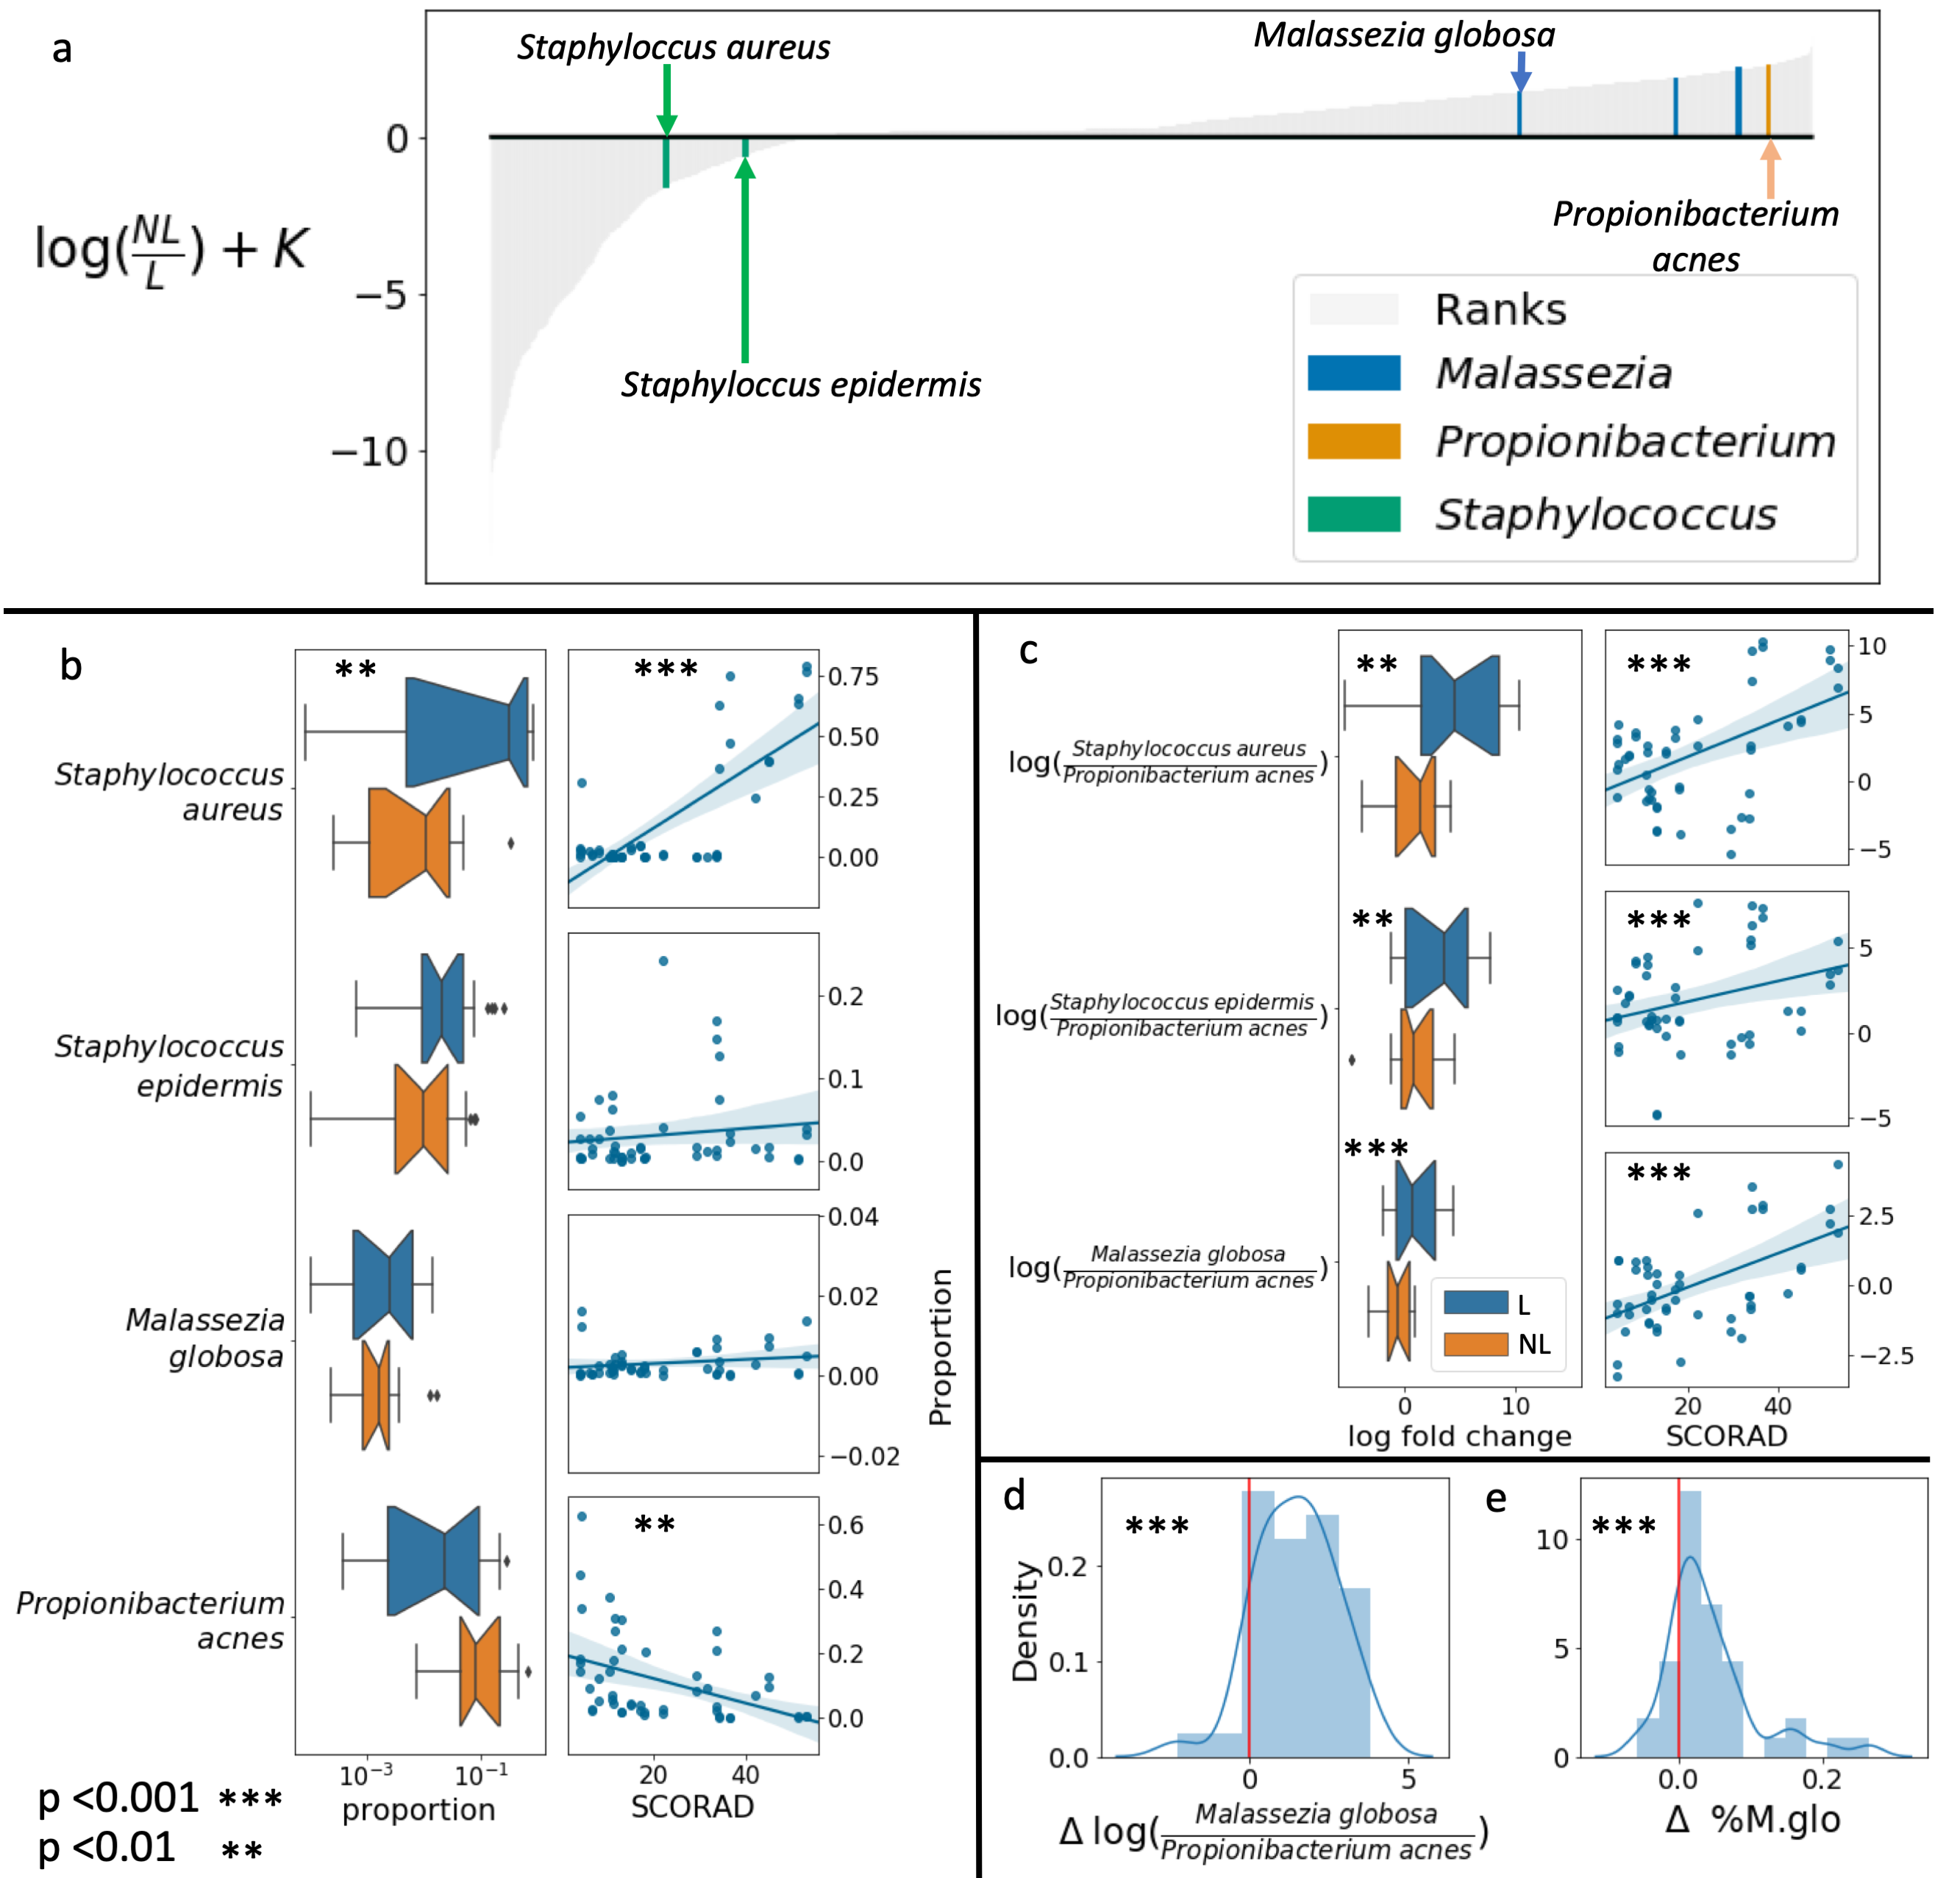
\includegraphics[width=1\textwidth]{ch4/Figure3.png}
  \caption[Analysis of lesion and non-lesion sites using proportions, log-ratios and ranks on two
    independent atopic dermatis cohorts.]{
    Comparison of lesioned (L) versus non-lesioned (NL) skin in two atopic dermatitis studies;
    Byrd et al.\cite{Byrd2017-eb}, (a-c) and Leung et al.\cite{Leung-DYM}, (d-e). (a) Microbial ranks estimated from
    multinomial regression applied to shotgun metagenomics from Byrd et al\cite{Byrd2017-eb} with key
    genera highlighted. The y-axis represents the log-fold change that is known up to some bias constant K.
    (b) Proportions of \textit{S. aureus}, \textit{S. epidermidis}, \textit{M. globosa}, and \textit{P. acnes}
    in lesioned (blue) and non-lesioned (orange) skin (left) and correlation of relative abundance
    with \gls{scorad} score (right) (c) Log-ratios of \textit{S. aureus} : \textit{P. acnes} , \textit{S. epidermidis} : \textit{P. acnes} ,
    and \textit{M. globosa} : \textit{P. acnes} (left) and correlation of ratio with \gls{scorad} score.
    (d) Change in log ratio of \textit{M. globosa} : \textit{P. acnes}. (e) Change in
    relative abundance of M. globosa between lesioned and non-lesioned skin from (Leung et al.\cite{Leung-DYM}).}
\end{figure}
%
To validate this observation, we analyzed shotgun data from another atopic dermatitis dataset (Leung et al. \cite{Leung-DYM}, under review).
Again, we found that although there was no difference in the proportion of M. globosa between lesioned and non-lesioned skin
(Fig. 3e), the ratio of \textit{M.globosa} : \textit{P.acnes} increased significantly in lesioned skin (t-statistic=$5.79$,
p-value=$8.6 \times 10^{-7}$) (Fig. 3d). These results are congruent with a previous finding that \textit{M. globosa}
was cultivated more successfully from lesioned versus non-lesioned sites in \gls{ad} \cite{Falk2005-we}. Analysis
differentials can identify a novel, clinically significant microbial interaction which can be validated
across cohorts by choosing insightful reference frames for measuring compositional change.\\[5 mm]
%
\section*{Discussion}
Adding information about absolute microbial load between samples can highlight issues inherent in compositional data
analysis. However, there are multiple practical and technical challenges in applying flow cytometry, \gls{qpcr}, or culturing
analyses to complex or low biomass sample types such as skin swabs. Fortunately, absolute abundances of a community
are only one dimension of measurement and there are robust, alternative techniques forgoing the need to estimate total
biomass. We have demonstrated the validity of using microbial ratios and ranked differentials to determine significant
changes in microbiome studies by comparing compositional inferences with absolute abundance inferences. \\[5 mm]
%
By using flow cytometry to quantify total microbial load, we were able to validate these analytical tools in 16S \gls{rrna} gene
amplicon sequencing data from unstimulated saliva. We found evidence of false positives when looking exclusively at changes
in relative abundance before and after brushing teeth. By looking at the ratio of \textit{Actinomyces} : \textit{Haemophilus}, we reached
an identical conclusion to our cell-count normalized data without the need for microbial load quantification. The
consistency of our results rests from the use of ratios defining reference frames for inferring compositional changes.
Other methods for inferring community compositional changes with different reference frames can be assumed to be
similarly reliable and bypass the need for costly and rate-limiting absolute abundance data.
%
Furthermore, we highlighted an example of a false negative in previously generated shotgun metagenomic data from the
skin of individuals with \gls{ad}. We were able to reproduce the findings that \textit{S. aureus}, and to a lesser extent S. epidermidis,
are differentially abundant in \gls{ad} lesions. Additionally, using log ratios and differential ranking, we were also able
to show a more subtle but statistically significant change in \textit{M. globosa} abundance in \gls{ad} lesions. This same result was
obtained in two independent metagenomic studies of \gls{ad} patients, and agrees with previous culturing-based work quantifying
increased colony forming units of \textit{M. globosa} in \gls{ad} lesions. \\[5 mm]
%
The seeming contradiction between microbial load-corrected abundances and relative abundances does not invalidate data
from the existing 40,000+ experiments utilizing 16S \gls{rrna} gene amplicon or metagenomic sequencing. Importantly, these
techniques are not limited to next generation microbiome sequencing, but can be applied to any experiments involving
compositional data (e.g. metabolomics, transcriptomics, proteomics, etc.). \\[5 mm]

While there are widespread misconceptions concerning how to interpret microbial abundances, there is still much
hope for resolving these outstanding controversies. Ongoing efforts at the NIH and EMBL-EBI have already stored
multiple petabytes of multi-omics datasets ready to re-analyze, databases such as Qiita contain curated data and
metadata from hundreds of thousands of samples \cite{Gonzalez2018-rv} , and there is much promise for resolving
the outstanding controversies by analyzing these datasets using reference frames to make stable inferences of
compositional change. \\[5 mm]
%
%
\section{Methods}
If we wanted to compute the change between two samples containing compositions (e.g. relative abundance of microbes) $\bm A=(a_1,...,a_D)$ and $\bm B=(b_1,...,b_D)$ , it would look like
\begin{align}
  \frac{\bm{A}}{\bm{B}}=\big(\frac{a_1}{b_1} ,\ldots  \frac{a_D}{b_D}\big)
\end{align}
If we are only able to measure relative abundances, as is the case with next generation amplicon sequencing, we can only estimate the proportion $p_{a_i}$ for species $i$ in the sample $A$  i.e. $p_{a_i}=\frac{a_i}{N_a}$.  Estimating the true abundance can be done via $a_1=N_a p_{a_1}$, where $N_a$ is the total abundance of sample $A$.  If we wanted to estimate the true change, that can be done as follows
\begin{align}
  \frac{\bm{A}}{\bm{B}} =
  \frac{N_a \times p_{a_1}}{N_b \times p_{b_1}}, \ldots \frac{N_a \times p_{a_D}}{N_b \times p_{b_D}} =
  \frac{\bm{p_A}}{\bm{p_B}} \times  \frac{\bm{N_A}}{\bm{N_B}}
\end{align}
If we wanted to determine if species $i$ abundance has changed between samples $A$ and $B$, we would want to test to see if $\frac{a_i}{b_i}=1$. However as shown above, we cannot perform this test, since the results of this test would be confounded by the total biomass bias $\frac{N_A}{N_B}$.\\[5 mm]
In many cases, the total biomass cannot be estimated, so any techniques to identify important species will need to alleviate this bias. One alternative is to use ratios. If we choose species D to be the reference species, it is clear that the total biomass cancels as follows
\begin{align}
  \frac{a_1/a_D}{b_1/b_D}  =  \frac{p_{a_1}/p_{a_D} }{p_{b_1}/p_{b_D}}
\end{align}
Another alternative is to use ranks. Since the bias is applied uniformly across the differential, it will not affect the ordering of the species. Hence, ranks are agnostic to the total biomass bias.
\begin{align}
  rank (\frac{\bm{A}}{\bm{B}}) =
  rank(\frac{\bm{p_A}}{\bm{p_B}} \times \frac{\bm{N_A}}{\bm{N_B}}) =
  rank(\frac{\bm{p_A}}{\bm{p_B}} )
\end{align}
This differential is also commonly referred to as a perturbation in the context of the compositional literature \cite{Pawlowsky-Glahn2015-qb}.
It is important to note that this does not justify using Spearman correlation or other non-parameteric tests such as Kruskal-Wallis applied to relative abundance data since these tests do not satisfy scale invariance \cite{Friedman2012-cn}.\\[5 mm]
%
Both of these techniques satisfy scale invariance, meaning that both of these techniques are agnostic to the total biomass.  This concept is critical when analyzing relative abundance data, since this is one step closer to maintaining consistent conclusions between the original environment and the observed sequences.\\[5 mm]
%
Estimating log-fold differential expression from relative abundances can result in either false positive (\gls{fp}) or false negatives (\gls{fn}) depending on the distribution of true differential expression. Whether \gls{fn}s or \gls{fp}s are observed depends on a nonlinear relationship involving the true (unobserved) differential expression. For a p-vector $x$ let us define $\gls{lse}(x) = \log(e^{x_1}+ \ldots +e^{x_p})$. If $\bm{\delta}=(\delta_1, \ldots ,\delta_D)$ denotes the true differential expression of the $D$ species between two conditions, let $\bm{\alpha}=\gls{lse}(\bm{\delta})$. Further, let $\hat{\bm{\delta}}=(\hat{\delta_1}, \ldots, \hat{\delta_D})$ represent the inferred differential expression from proportional data and $\bm{\hat{\alpha}}=\gls{lse}(\bm{\hat{\delta}})$. If $\gls{lse}(\delta) > \gls{lse}(\hat{\delta})$ then \gls{fp}s will be observed. In contrast if $\gls{lse}(\delta) < \gls{lse}(\hat{\delta})$ then \gls{fn}s will be observed.\\[5 mm]
%
\subsection{Saliva sample collection}
Eight volunteers provided unstimulated saliva so that salivary flow rate could be measured according to a standardized protocol \cite{Navazesh2008-me}. Briefly, individuals were asked to allow saliva to flow for exactly five minutes through a disposable funnel (Simport, SIM F490-2)into a sterile, 15 mL conical tube preloaded with 2 mL sterile glycerol for bacterial preservation. Participants were asked to provide samples before brushing and after brushing teeth in the morning and in the evening. Samples inverted several times to mix with the glycerol and stored at -20$\degree$C immediately after collection. This study was approved by an Institutional Review Board (IRB\# 150275) and written informed consent was acquired before sample collection\\[5 mm]
%
\subsection{Flow cytometry}
Unstimulated saliva samples were thawed on ice, and aliquots were diluted tenfold with sterile, 1x PBS. To remove human cells and salivary debris, samples were filtered using a sterile 5 $\mu$m syringe filter (Sartorius Stedim Biotech GmbH). 5 $\mu$l 20x SYBR green (SYBR$^{TM}$ Green I Nucleic Acid Gel Stain, Invitrogen) was added to 1 mL of the microbial suspension (0.1x final concentration) and incubated in the dark for 15 minutes at 37$\degree$C.  Finally, 50 $\mu$l AccuCount Fluorescent Particles (Spherotech, AC\gls{fp}-70-10) were added for assessment of microbial load. Sample were processed on a SH800 Cell Sorter (Sony Biotechnology) using a 100 $\mu$m chip with the threshold set on FL1 at 0.06\%, and gain settings as follows; FSC=4, BSC=25\%, FL1=43\%, FL4=50\%. The gating strategy was adapted from Vandeputte et al.,\cite{Vandeputte2017-jl}. Briefly, fluorescent microbial cells were gated from background on a FL1-Fl4 density plot, and remaining background was removed by eliminating large events detected on a FSC-BSC density plot. Negative controls (sterile PBS stained identically to samples) was run between each sample set to exclude cross-contamination. Settings were identical among all samples.\\[5 mm]
%
\subsection{Amplicon sequencing}
DNA extraction and 16S \gls{rrna} amplicon sequencing were done using Earth Microbiome Project (EMP) standard protocols (http://www.earthmicrobiome.org/protocols-and-standards/16s). 500 $\mu$l of unstimulated saliva was used for gDNA extraction with MagAttract PowerSoil DNA Kit (QIAGEN) as previously described \cite{Marotz2017-dy}. Amplicon PCR was performed on the V4 region of the 16S \gls{rrna} gene using the primer pair 515f to 806r with Golay error-correcting barcodes on the reverse primer. 240 ng of each amplicon was pooled and purified with the MO BIO UltraClean PCR cleanup kit and sequenced on the Illumina MiSeq sequencing platform.\\[5 mm]
The sequences and biom tables \cite{McDonald2012-xw} can be found on Qiita (http://qiita.microbio.me) under study ID 11896. Demultiplexed fastq files were processed using QIIME2 (https://qiime2.org)\cite{Caporaso2010-nm}.  Deblur was used to denoise the sequences \cite{Amir2017-zw}.  16S taxonomy was assigned using RDP classifier \cite{Pawlowsky-Glahn2015-qb,Wang2007-gj}. Songbird was used to perform multinomial regression - repository can be found here: https://github.com/mortonjt/songbird\\[5 mm]
Paired t-tests were performed to evaluate the differences before and after brushing teeth.
All log-ratios that were evaluated to either positive or negative infinity are dropped prior to statistical analysis.
These numerical issues occur due to particular microbes not observed, and we treat them as missing data respectfully.
%
\subsection{Shotgun metagenome studies}
We used supplementary data from Byrd et al \cite{Byrd2017-eb} and Donald Leung\cite{Leung-DYM}. The provided relative abundances were compared to the log ratio of the raw count data. Paired t-tests were performed to evaluate the differences between lesion and non-lesion skin samples.
All log-ratios that were evaluated to either positive or negative infinity are dropped prior to statistical analysis.
These numerical issues occur due to particular microbes not observed, and we treat them as missing data respectfully.

\section{Acknowledgements}
We would like to Doris Vandeputte for her insights behind the total microbial load quantification.
J.T.M. was funded by NSF GR\gls{fp} DGE-1144086.

%
%
%%% APPENDIX
\appendix
\chapter{Supplemental material for Chapter 2}
\begin{figure}[H]
        \centering
        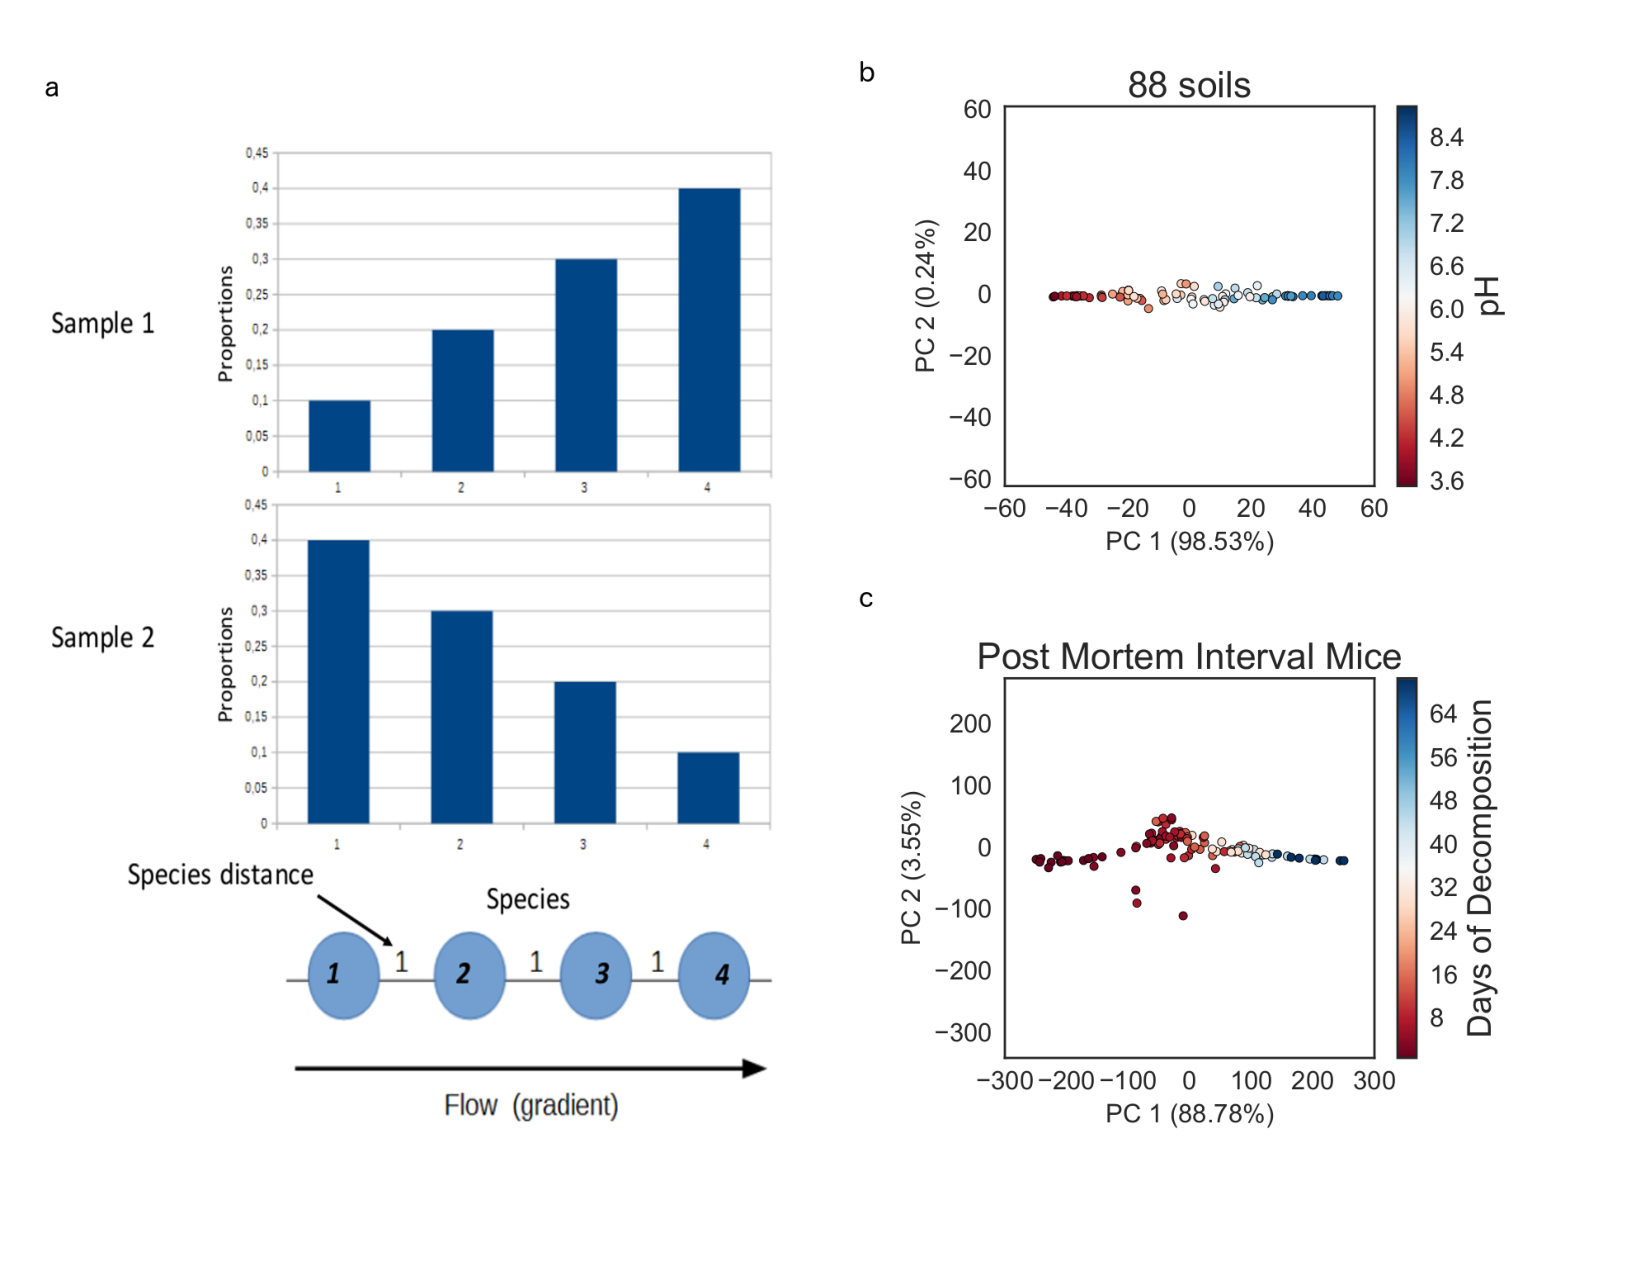
\includegraphics[width=1\textwidth]{appendix_a/FigureS1.pdf}
        \caption[An illustration of a distance metric that is engineered not to saturate.]{(a) An illustration of the Earth Mover Band Distance.  (b)  Demonstration of the EMBAD metric on the 88 soils dataset.
          (c) Demonstration of the EMBAD metric on the Post Mortem Interval Mice dataset}
        \label{figaS1}
\end{figure}
The idea behind the EMBAD distance metric is as follows.  Suppose that we have obtained a scrambled matrix of OTU abundances but there exists an underlying band pattern when the table is sorted.  Specifically, this table can be reordered and sorted by a value, such as sample pH.  In addition, the species can also be sorted by the sample value ranges that they are observed in.  In the pH example from the 88 soils study, the microbes (OTUs) were ordered based on the pH ranges they were found in.  This ordering of species can be used to construct a pipe where the lowest ordered species is placed on one end of the pipe, and the highest ordered species is placed on the opposite end of the pipe.  Once this pipe is constructed the species abundances from different samples can be imposed on the pipe, and the flow between samples can be computed using the Earth Mover’s distance.  Consider the example in Figure S1a.  There are two samples where sample 1 is dominated by species 4 and sample 2 is dominated by species 1.  If the ordering of species is already known, we can compute the proportions of individuals in sample 1 that need to be shuttled along the pipe in order to transform sample 1 into sample 2.  In this scenario, about 0.3 of species 1, 0.1 of Species 3 need to be distributed across species 1 and 2.  If we can determine the ordering of species, we can effectively compute how dissimilar Sample 1 and Sample 2 are from each other.\\[5 mm]
 Furthermore, by imposing an ordering across all species, this distance metric is designed to be non-saturating.  If there are samples that do that overlap, the dissimilarity between these samples is weighed by how far away they are in the pipe.  Two samples that appear close together in the pipe will have a smaller distance since there the proportions will travel a smaller distance along the pipe.\\[5 mm]
%
 \begin{figure}[H]
         \centering
         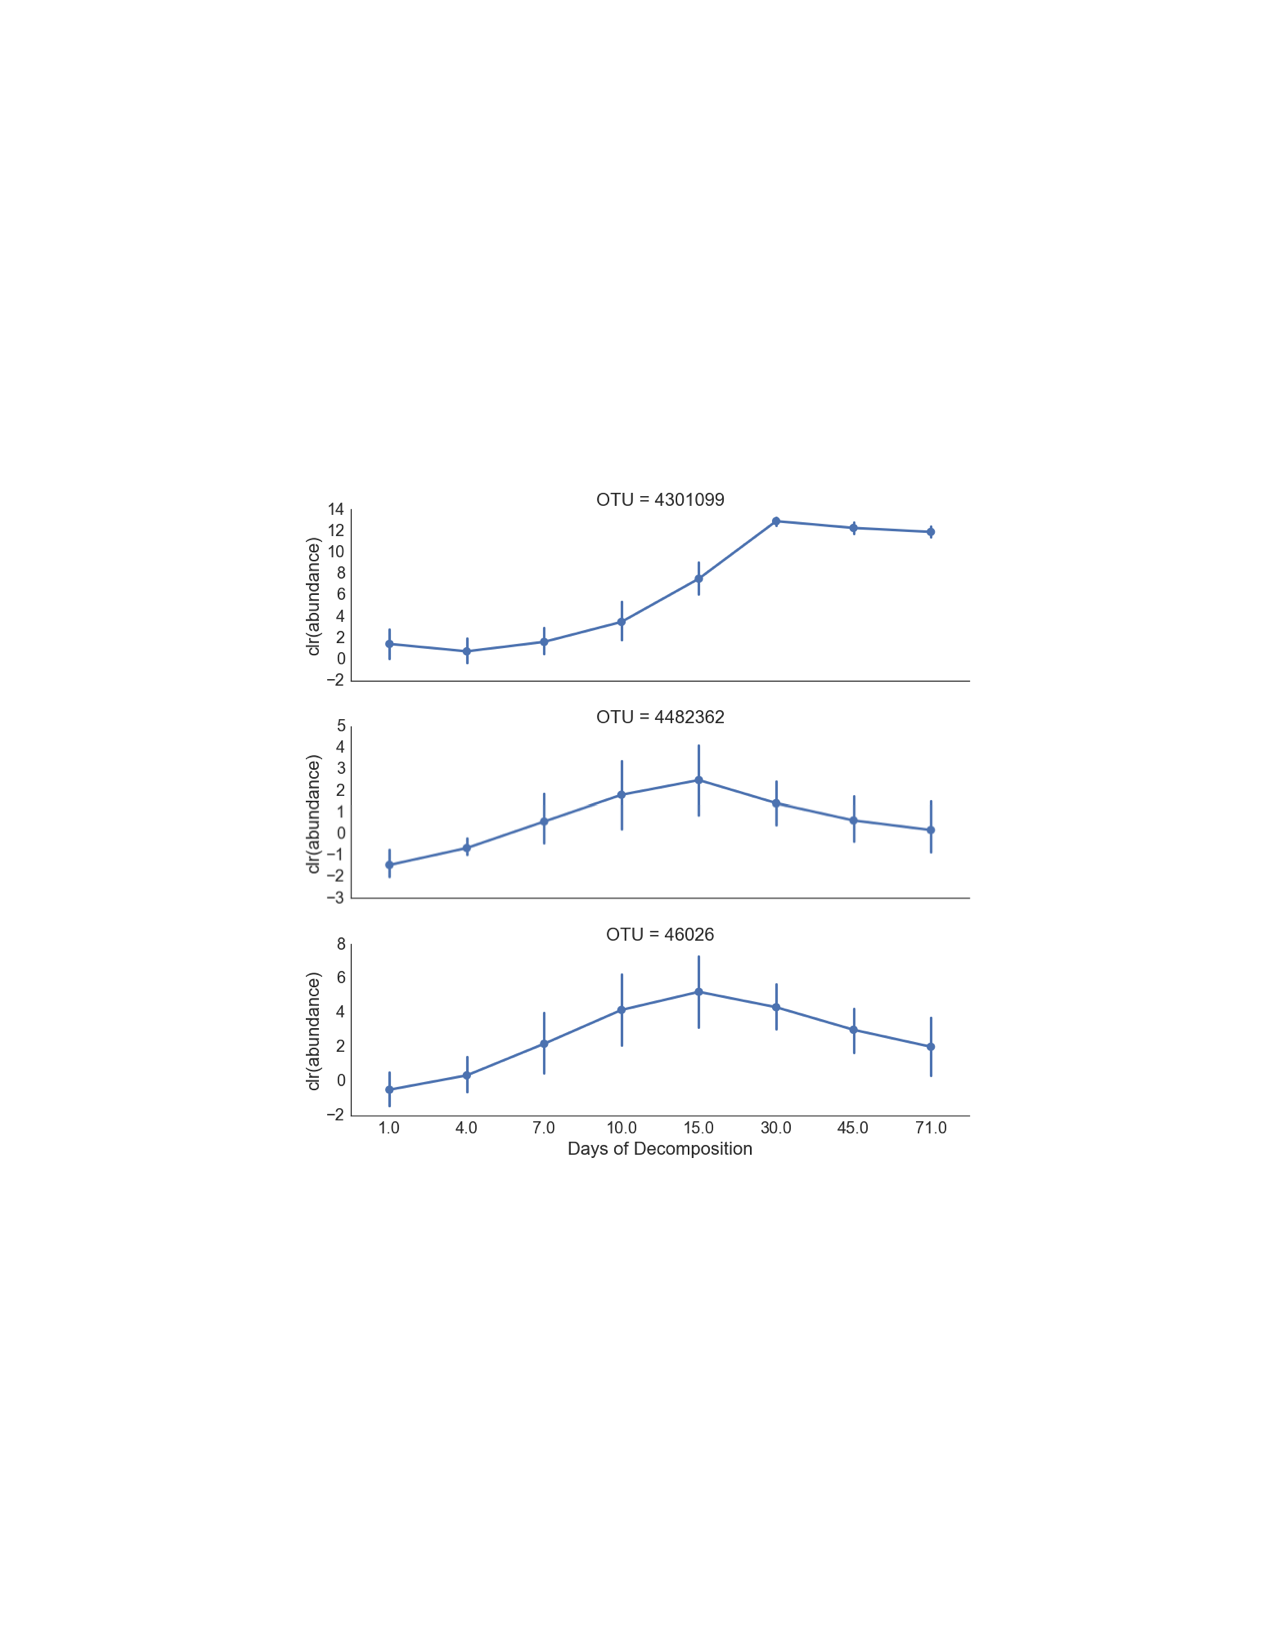
\includegraphics[width=1\textwidth]{appendix_a/FigureS2.pdf}
         \caption[Abundances of taxa across time in the post-mortem experiment.]
         {The center log ratio (Equation 2) transformed abundances of Rhizobiaceae (OTU 4301099) and Chromatiaceae (OTU 46026, 4482362) versus time. These demonstrate distinct relationships of different taxa as a function of decomposition.}
         \label{figaS2}
 \end{figure}
%
 \section{Distance saturation proof}
 \textbf{Theorem:}\\
 Let $(S_i)_{1 \leq i \leq N}$ be a set of $N$ different samples along a linear trajectory\\[5 mm]
 Let $d=\min_{i, j, i \neq j} \lVert S_i - S_j \rVert_2$ be the minimum Euclidean distance between every pair of samples in $(S_i)_{1 \leq i \leq N}$ and $C=\max_{i, j} \lVert S_i - S_j \rVert_2$ be the maximum Euclidean distance between every pair of samples in $(S_i)_{1 \leq i \leq N}$.\\
 We have
 \[ N \leq \bigg\lfloor \frac{C}{d} \bigg\rfloor +1\]
 \textbf{Proof:}\\
 Since all our samples samples are on a linear trajectory, without loss of information we can
 project the samples on this line.  Now consider our samples as points in $\mathbb{R}$ the
 real number line. \\[5 mm]
 Without loss of generality, we can suppose that our samples are ordered long the real line:
 \[S_1<S_2<\cdots<S_N\]
 We have $d>0$ because all samples are different.\\
 Thanks to the structure of the real line, we have
 \[C=\max_{i, j} \lVert S_i - S_j \rVert_2 = S_n-S_1\]
 and all samples are part of the interval of length $C:I=[S_1,S_n ]$\\
 We can include the interval $I$ into the reunion of $\lfloor \frac{C}{d} \rfloor +1$ intervals of length $d$.\\
 Since $d=\min_{i, j, i \neq j} \lVert S_i - S_j \rVert_2$ two samples cannot be in the same
 sub-interval $I_k$. \\
 Therefore by the pigeon-hole principle\\
  \[ N \leq \bigg\lfloor \frac{C}{d} \bigg\rfloor +1\]
\textbf{Corollary:}\\
When there is a distance-saturation, we have $N \leq \bigg\lfloor \frac{C}{d} \bigg\rfloor +1$, therefore $N$ samples cannot be on a linear trajectory.\\[5 mm]

\section{NP hardness of finding an optimal linear embedding}
Suppose that we have a scrambled table and has an underlying band pattern. \\[5 mm]
In order to define an EMBAD distance to infer an underlying band pattern in the absence of a known gradient, we need to (1) be able to determine the define the trajectory of points that define the horseshoe and (2) determine the optimal ordering of OTUs based on (1). In order to resolve (1), we need to obtain the shortest path through the horseshoe.  Specifically we would need to find the optimal ordering of points $x_1, \ldots ,x_N \in \mathbb{R}^D_+$ such that the following objective function is minimized.
\[ \min \sum\limits_{i=1}^n \lVert x_i - x_{i-1} \rVert_2 \]
If there exists an algorithm to find the shortest path through the horseshoe, then this solution can be used to solve the Traveling Salesman problem.  Therefore, defining an EMBAD distance metric in the absence of a known gradient is NP-hard.


\chapter{Supplemental material for Chapter 3}
\section{Scale invariance of balances}
\begin{align}
\log \frac{\prod_{x_j \in i_L}{(x_j)^{1/|i_L|}}}{\prod_{x_k \in i_R}{(x_j)^{1/|i_R|}}} =
\log \frac{\prod_{p_j \in i_L}{(\textcolor{red}{n}p_j)^{1/|i_L|}}}{\prod_{p_k \in i_R}{(\textcolor{red}{n}p_j)^{1/|i_R|}}}=
\log \frac{\prod_{p_j \in i_L}{(p_j)^{1/|i_L|}}}{\prod_{p_k \in i_R}{(p_j)^{1/|i_R|}}}
\end{align}
$n$  is the true sequencing count, $x_j$ is the true abundances of species $j$ and $p_j$ is the proportion of species $j$. $i_L$ is the set of all species proportions contained in the left sub-tree at internal node $i$, $i_R$ is the set of all species proportions contained in the right sub-tree at the internal node $i$, and, $g(x)$ is the geometric mean of all of the proportions contained in $x$, $|i_R|$ is the number of species contained  $i_R$ and  $|i_L|$ is the number of species contained  $i_L$.  As shown above, the sequencing depth constant gets effectively canceled out.  Thus, log ratios are a natural normalization for sequencing depth, especially if there are no zero abundances present and the samples have sufficient coverage.

%
\section{Benchmark of compositional coherence}
\textbf{Supplemental Figure 1}

The simulation consisted of a uniform population of 1000 individuals.  A blooming was simulated across 9 time points, where a single organism eventually grew 100,000x fold.  At each time point, 30 compositions were simulated using multinomial sampling with replacement.  At each time point, a statistical test was performed comparing the sample at that time point to the original time point.  Since we know beforehand that only 1 species is changing, any other tests that don’t involve the first set of proportions that is determined to be significant with p-value $<$ 0.05 is a false positive Figure S1a-b).  In fact, if the bloom of a given species is high enough, all of the other individuals can be detected to change.  In Figure S1e, if 1 species has changed by 100,000x, then all of the pvalues will be less than 10-10, giving a false positive rate close to 100\%.  The same procedure is performed using balances, any balance that does not contain x1 that is determined to be significant from a t-test is considered a false positive (Figure S1c).  Note that this is highly dependent on the choice of the tree.  In this case, we used a tree where the blooming species x1 was to the far right of the tree (Figure S1f).  In this way, only the balance between x1, and x2 through x1000 should be changing.  But if we were to flip the tree, and place x1 to the far right of the tree, every balance in the tree will contain x1 (Figure S1g).  So as x1 blooms, the number of significant balances will increase (Figure S1d).

\begin{figure}[H]
        \centering
        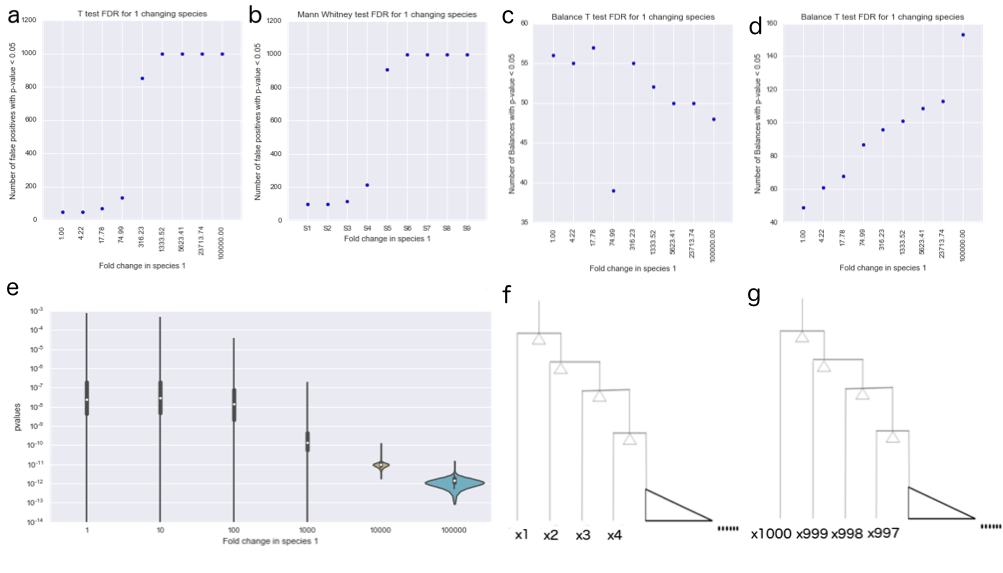
\includegraphics[width=1\textwidth]{appendix_b/sup_figure1.png}
        \caption[A benchmark of statistical tests on compositional data.]{Simulations illustration the occurence of false positives in
          traditional statistical tests}
        \label{figbS1}
\end{figure}
While it may be deemed biologically irrelevant, blooms do happen frequently in microbial studies, with individual species sometimes blooming 5 orders of magnitude within a short period of time.  And the 10,000x fold growth of a single species will have the exact same effect as the 1,000x fold growth change of 10 species.  This suggests that there could be many subtle scenarios where we could be misinterpreting biologically relevant signals by testing individual proportions of microbes.\newpage
\textbf{Supplemental Figure 2}

\begin{figure}[H]
        \centering
        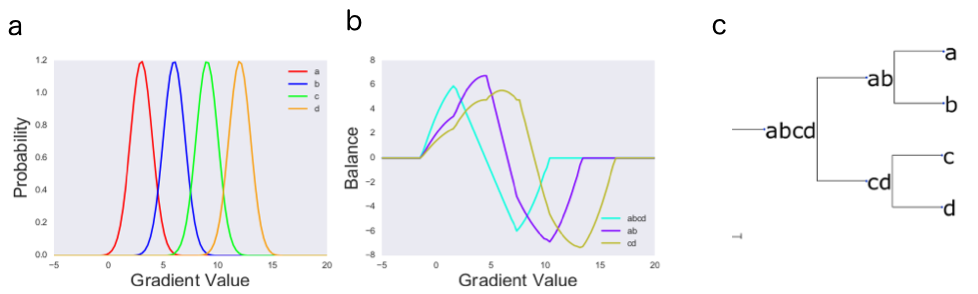
\includegraphics[width=1\textwidth]{appendix_b/sup_figure2.png}
        \caption[An ecological intrepretation of balances]{A simulation of 4 species, where each species is normally distributed along some environmental gradient.  Each species has a normal distribution with a variance of 3 and a mean of 3, 6, 9 and 12 respectively as shown in Figure S2a.  The resulting balances can be calculated as follows.}
        \label{figbS2}
\end{figure}
\[
abcd = \log \frac{\sqrt{ab}}{\sqrt{cd}} \qquad
ab = \log \frac{\sqrt{a}}{\sqrt{b}}
cd = \log \frac{\sqrt{c}}{\sqrt{d}}
\]
Note, it is not possible to take a logarithm of zero.  A commonly used approach around this problem is to add a pseudocount.  Here we add a pseudocount of 1 after multiplying all of the species probabilities by 10000.  These species abundances are transformed into balances as shown in Figure S2b.  Because of the zero phenomenon, the balances yield something reminiscent to a triangular wave when applied to a pair of unimodal distributions.  Take balance ab for example.  At the far left around -5, neither a or b are present, so both of their abundances are zero.  But since we are adding pseudocounts, the resulting balance is given by log(1/1)=0 . When the gradient value increases to 0, the abundance of a approaches the peak of the distribution, while the abundance of b is still zero, causing the ab balance to increase.  By the time the gradient value is around 4, the abundances of b starts to appear, causing the ab to peak.  When the gradient value is around 8, the abundance of a starts disappearing while the abundance of b starts approaching the maximum peak in Figure S2a.  At a gradient value of 10, the abundance of b also begins to dwindle, and the ab balance spirals towards zero.  This same triangular wave pattern appears in all 3 of these balances, and portions of this also appear in the 88 soils study as shown in Figure S3.

It is also important to note that a balance of zero also indicates that the abundances between the ratios are equal.  So if a balance is zero, and a pseudocount scheme was used, either the proportions between the numerator and denominator are truly equal, or both the numerator and the denominator are zero.\newpage
\section{Analysis of balances in soils}
\textbf{Supplemental Figure 3}

\begin{figure}[H]
        \centering
        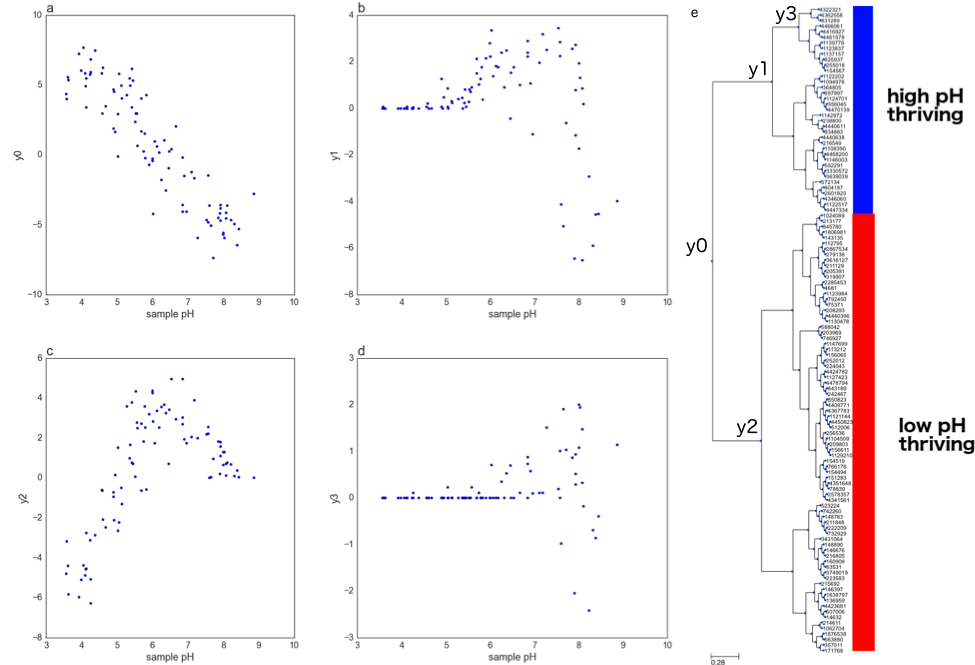
\includegraphics[width=1\textwidth]{appendix_b/sup_figure3.png}
        \caption[Other balances from the 88 soils study.]{A perspective of different balances in the 88 soils study.}
        \label{figbS3}
\end{figure}

If there is truly a unimodal species distribution along pH, we’d expect to see the same sort of triangular wave pattern as shown in Figure 2S.  If this is the case, then the top balance y0 is likely to be resulting from the midsection of the triangular wave between the minimum and the maximum (Figure S3a).  The peaks of the triangular wave are a bit more apparent in the Figure S3b-d.  In Figure S3b, the lower subtree in y1 is probably reaching a maximum in the true abundance around a pH of 7.  In Figure S3c, the upper subtree in y2 is also likely approaching a maximum in the true abundance around a pH of 6.  The same sort pattern could be happening in Figure S3d with the lower subtree in y3.  These glimpses of triangular waves in these graphs suggest that there could be unimodel distributions of OTUs across the pH gradient.

As daunting as the zeros problem is, the zeros present in data sets such as the 88 soils follow predictable patterns.  Even with a simple pseudo count strategy, we can still extract sensible information about balances of microbes across different pH values.


\chapter{A brief overview of Aitchison Geometry}
Given that many of the techniques presented in the dissertation were based on the concepts based on Aitchison geometry, we will provide a brief overview behind Aitchison geometry.\\[5 mm]
%
Aitchison geometry is a framework focused on the analysis of quantities including proportions, percentages, probabilities and concentrations.  These quantities are also referred to as compositions.  At the heart of the framework is the characterization of the Aitchison simplex, where each element of the space is a composition.  A composition can be thought of as a set of proportions, or percentages.\\[5 mm]
%
Linear operations can be defined on compositions, known as ``perturbation'' and ``powering operations''.  These operations are linear in the Aitchison simplex and can be transformed into traditional addition and multiplication operations in Euclidean space through the use of log-ratio transformations.  Inner products can be defined in the Aitchison simplex, giving rise to the distance metrics such as the Aitchison distance.  It can also be shown that the Aitchison simplex forms a finite Hilbert space \cite{Pawlowsky-Glahn2015-qb}. \\[5 mm]
%
\section{Definition}
The Aitchison simplex is formally defined for D species as follows
\[\mathcal{S}^D=\left\{\mathbf{x}=[x_1,x_2,\dots,x_D]\in\mathbb{R}^D \,\left|\, x_i>0,i=1,2,\dots,D; \sum_{i=1}^D x_i=\lambda \right. \right\}. \]
Where $\lambda>0$ can be any positive real-valued constant.  By definition, the compositions are the quantities denoted by $\mathbf{x}$.

 \begin{figure}[H]
         \centering
         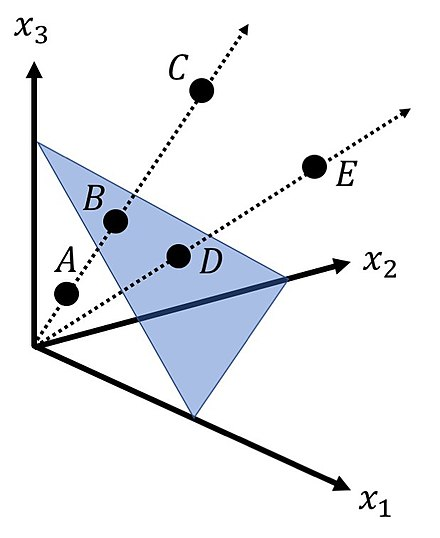
\includegraphics[width=0.5\textwidth]{appendix_c/Aitchison-simplex.jpg}
         \caption[An illustration of the Aitchison simplex.]
                 {An illustration of the Aitchison simplex.  Here, there are 3 parts, $x_1, x_2,  x_3$ represent values of different proportions.  A, B, C, D and E are 5 different compositions within the simplex.  A, B and C are all equivalent and D and E are equivalent.}
         \label{figcS1}
 \end{figure}
There are three core axioms that the Aitchison simplex, namely

\subsection{Scale invariance}
Whether data is represented as proportions, percentages or probabilities, in the context of the Aitchison simplex all of these measurements are equivalent since they only differ by a constant scaling factor.

\subsection{Subcompositional coherence}
Observations on shared species should be consistent. For example, supposed that there are 2 biologists that visited the exact same rainforest to count insects.  One biologist observed 3 species of spiders and 10 species of ants whereas the other biologist only observed 2 species of spiders and 7 species of ants.  If these biologists observed the same 2 spider species and the same 7 species of ants, their conclusions about those species should be the same.  For instance, they should notice that the ratio of those two spider species are consistent between their observations.  While the universal formal definition is still not clearly established, this concept can be formalized to distance metrics as follows

  \[
d(x_k, y_k) \leq d(x, y) \qquad
\forall x, y \in S^D, \; x_k, y_k \in S^k, \; S^k \subset S^D
\]

\subsection{Permutation invariance}
The ordering of how the proportions or were measured or counted doesn't matter.  This is analogous to how combinations are invariant to the order of selection.


\section{Vector Space Structure}
\subsection{Properties}
The Aitchison simplex has the following operators defined using the \textbf{closure} operation as follows

\subsubsection{Perturbation}
\[ x \oplus y = [\frac{x_1 y_1}{\sum_{i=1}^D x_i y_i},\frac{x_2}{\sum_{i=1}^D x_i y_i}, \dots,\frac{x_D y_D}{\sum_{i=1}^D x_i y_i}] =
C[x_1 y_1, ..., x_D y_D]  \qquad \forall x, y \in S^D
\]

\subsubsection{Powering}

\[
\alpha \odot x = [\frac{x_1^{\alpha}}{\sum_{i=1}^D x_i^{\alpha}},\frac{x_2^{\alpha}}{\sum_{i=1}^D x_i^{\alpha}}, \dots,\frac{x_D^{\alpha}}{\sum_{i=1}^D x_i^{\alpha}}] =
C[x_1 y_1, ..., x_D y_D]  \qquad \forall x \in S^D, \quad \alpha \in \mathbb{R}
\]

\subsubsection{Inner product}

\[
\langle x, y \rangle = \frac{1}{2D}
\sum\limits_{i=1}^{D}
\sum\limits_{j=1}^{D}
\log \frac{x_i}{x_j}
\log \frac{y_i}{y_j}
\qquad \forall x, y \in S^D
\]

Under these these operations alone, it is sufficient to show that the Aitchison simplex forms a Euclidean vector space.

\subsection{Orthonormal bases}
Since the Aitchison simplex forms a finite Hilbert space, it is possible to construct orthonormal bases in the simplex. Every composition can be decomposed as follows

\[ x = \bigoplus_{i=1}^D x_i \odot e_i \]

Where $e_1, \ldots e_{D-1} $ forms an orthonormal basis in the simplex \cite{ilr}.

\section{Linear transformations}

There are 3 well-characterized isomorphisms that transform from the Aitchison simplex to real space.  All of these transforms satisfy linearity and as given below

\subsection{Additive Logratio Transform}
The additive log ratio (alr) transform is an where $alr: S^D \rightarrow \mathbb{R}^{D-1} $.  This is given by

\[ alr(x) = \big[ \log \frac{x_1}{x_D} \ldots \log \frac{x_{D-1}}{x_D} \big]\]

The choice of denominator component is arbituary, and could be any specified component.
This transform is commonly used in chemistry with measurements such as pH.  In addition, this is the transform most commonly used for Multinomial logistic regression.  The alr transform is not an isometry, meaning that distances on transformed values will not be equivalent to distances on the original compositions in the simplex.

\subsection{Center Logratio Transform}
The center log ratio (clr) tranform is both an isomorphism and an isometry where \\$clr: S^D \rightarrow \mathbb{U}, \quad U \subset \mathbb{R}^{D} $

\[clr(x) = \big[ \log \frac{x_1}{g(x)} \ldots \log \frac{x_{D-1}}{g(x)} \big] \]

The inverse of this function is also known as the softmax function commonly used in neural networks.

\subsection{Isometric Logratio Transform}
The isometric log ratio (ilr) tranform is both an isomorphism and an isometry where $ilr: S^D \rightarrow \mathbb{R}^{D-1} $

\[
ilr(x) = \big[ \langle x, e_1 \rangle, \ldots \langle x, e_{D-1} \rangle]
\]

There are multiple ways to construct orthonormal bases, including using the Gram–Schmidt process Singular-value decomposition of clr transformed data.
Another alternative is to construct log contrasts from a bifurcating tree.  If are given a bifurcating tree, we can construct a basis from the internal nodes in the tree.

 \begin{figure}[H]
         \centering
         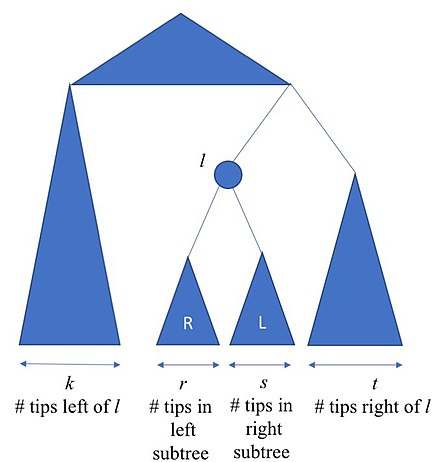
\includegraphics[width=0.5\textwidth]{appendix_c/Orthogonal-tree-basis.jpg}
         \caption[An illustration of the bifurcating trees as an orthonormal basis.]
                 {A representation of a tree in terms of its orthogonal components. l represents an internal node, an element of the orthonormal basis. This is a precursor to using the tree as a scaffold for the ilr transform.}
         \label{figcS1}
 \end{figure}

Each vector in the basis would be determined as follows

\[e_l = C[exp( \underbrace{0,...0}_{k}, \underbrace{a,...,a}_{r},\underbrace{b,...,b}_s,\underbrace{0,...0)}_t]\]

The elements within each vector are given as follows

\[a = \frac{\sqrt{s}}{\sqrt{r(r+s)}} \quad \textrm{and} \quad b = \frac{-\sqrt{r}}{\sqrt{s(r+s)}}\]

where $k, r, s, t$ are the respective number of tips in the corresponding subtrees shown in the figure.  It can be shown that the resulting basis is orthonormal \cite{groups_of_parts}.

Once the basis $\Psi$ is built, the ilr transform can be calculated as follows

\[
ilr(x) = C[\exp(clr(x) \Psi)]
\]


where each element in the ilr transformed data is of the following form


\[
b_i = \sqrt{\frac{rs}{r+s}} \log \frac{g(x_R)}{g(x_S)}
\]

where $ x_R$ and $ x_S$ are the set of values corresponding to the tips in the subtrees $R$ and $S$.


%% END MATTER
\printindex %% Uncomment to display the index
% \nocite{}  %% Put any references that you want to include in the bib
%               but haven't cited in the braces.
%\setlength{\bibleftmargin}{0.25in}  % indent each item
%\setlength{\bibindent}{-\bibleftmargin}  % unindent the first line
%\def\baselinestretch{1.0}  % force single spacing
%\setlength{\bibitemsep}{0.16in}  % add extra space between items
\bibliographystyle{unsrt}
\bibliography{template}  %% This looks for the bibliography in template.bib
%                          which should be formatted as a bibtex file.
%                          and needs to be separately compiled into a bbl file.


\end{document}

